\newglossaryentry{psd}
{name={positive semi-definite (psd)},
	description={A\index{positive semi-definite (psd)} (real-valued) 
		\gls{symmetricmatrix} $\mQ = \mQ\,^{T} \in \mathbb{R}^{\featuredim \times \featuredim}$ 
	 	 is referred to as psd if $\featurevec\,^{T} \mQ \featurevec \geq 0$ 
		for every \gls{vector} $\featurevec \in \mathbb{R}^{\featuredim}$. 
		A psd matrix $\mQ$ admits a \gls{spectraldecomp} with nonnegative 
		\glspl{eigenvalue} $\eigval{1}, \,\ldots, \,\eigval{\featuredim} \geq 0$
		\cite{HornMatAnalysis}, \cite{Axler2025}. 
	 	The notion of being psd can be extended from \glspl{matrix} to (real-valued) 
	 	symmetric \gls{kernel} \glspl{map} $\kernel: \featurespace \times \featurespace \rightarrow \mathbb{R}$ 
	 	(with $\kernel(\featurevec,\featurevec') = \kernel(\featurevec',\featurevec)$)
	 	as follows: For any finite set of \glspl{featurevec} $\featurevec^{(1)}, \,\ldots, \,\featurevec^{(\samplesize)}$, 
	 	the resulting \gls{matrix} $\mQ \in \mathbb{R}^{\samplesize \times \samplesize}$ with 
		entries $Q_{\sampleidx,\sampleidx'} = \kernelmap{\featurevec^{(\sampleidx)}}{\featurevec^{(\sampleidx')}}$ 
		is psd \cite{LearningKernelsBook}.
			\\
		See also: \gls{symmetricmatrix}, \gls{kernel}.},
	first={positive semi-definite (psd)},
	type=math, 
	text={psd}  
}

\newglossaryentry{normalmatrix}
{name={normal matrix},
	description={A normal \gls{matrix} is a square \gls{matrix} $\mA \in \mathbb{C}^{\nrfeatures \times \nrfeatures}$ 
                 that commutes with its \gls{conjugatetranspose}, i.e., $\mA\mA^{H}=\mA^{H}\mA$. 
                 Normal \glspl{matrix}\index{normal matrix} admit an orthonormal basis of \glspl{eigenvector} and are 
                 unitarily \gls{diagonalizable}.
                 \\
                 See also: \gls{matrix}, \gls{diagonalizable}. },
	first={normal matrix},
    	type=math, 
	plural={normal matrices},
	firstplural={normal matrices},
	text={normal matrix}
}

\newglossaryentry{spectraldecomp}
{name={spectral decomposition},
	description={Every \gls{normalmatrix} $\mA \in \mathbb{C}^{\nrfeatures \times \nrfeatures}$ 
                 admits\index{spectral decomposition} a spectral decomposition of the form 
                 \cite{HornMatAnalysis}, \cite{Axler2025}
       		\begin{equation}
             		\mA = 
              		\big( \vu^{(1)}, \,\cdots, \,\vu^{(\nrfeatures)}\big)
              		\begin{pmatrix}
              			\eigval{1} &        &        & 0\\
                      		& \eigval{2} &     &  \\
                      		&        & \ddots &  \\
              			0         &        &        & \eigval{\nrfeatures}
		 	\end{pmatrix}
              		\begin{pmatrix}
              			\big(\vu^{(1)}\big)^{H}\\
             		 	\vdots\\
             			\big(\vu^{(\nrfeatures)}\big)^{H}
		 	 \end{pmatrix}
			= \sum_{\featureidx=1}^{\nrfeatures} \eigval{\featureidx} \vu^{(\featureidx)} \big(\vu^{(\featureidx)})^{H} \nonumber \\ 
       		\end{equation}
      		with an orthonormal basis $\vu^{(1)},\,\ldots,\,\vu^{(\nrfeatures)}$. 
		Each basis element $\vu^{(\featureidx)}$ 
		is an \gls{eigenvector} of $\mA$ with a corresponding \gls{eigenvalue} $\eigval{\featureidx}$, 
		for $\featureidx=1,\,\ldots,\,\nrfeatures$ (see Fig. \ref{fig:eigenvectors-length_dict}).
       		\begin{figure}[H]
            		\centering
            		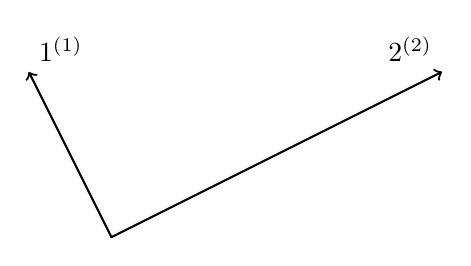
\begin{tikzpicture}[scale=2.1, line cap=round, line join=round]
            		% two eigenvectors with different lengths
            		\draw[->, thick] (0,0) -- (-0.5,1) node[above right] {$\eigval{1} \vu^{(1)}$};
           		 \draw[->, thick] (0,0) -- (2.0,1) node[above left]  {$\eigval{2} \vu^{(2)}$};
            		\end{tikzpicture}
            	\caption{The spectral decomposition of a \gls{normalmatrix} $\mA$ provides 
			an orthonormal basis $\vu^{(1)}, \vu^{(2)}$. Applying $\mA$ 
			amounts to a scaling of the basis \glspl{vector} by the 
			\glspl{eigenvalue} $\eigval{1},\eigval{2}$.\label{fig:eigenvectors-length_dict}}
		\end{figure}
		See also: \gls{normalmatrix}, \gls{eigenvector}, \gls{eigenvalue}. },
	first={spectral decomposition},
    	type=math,
	text={spectral decomposition}
}

\newglossaryentry{symmetricmatrix}
{name={symmetric matrix},
	description={A symmetric \gls{matrix} is a square\index{symmetric matrix} \gls{matrix} $\mA$ 
		with real-valued entries that is equal to its \gls{transpose}, i.e., $\mA=\mA^{T}$. Every 
		symmetric \gls{matrix} is a \gls{normalmatrix}.
                 \\
                 See also: \gls{transpose}, \gls{normalmatrix}. },
	first={symmetric matrix},
	plural={symmetric matrices},
    	type=math,
	firstplural={symmetric matrices},
	text={symmetric matrix}
}

\newglossaryentry{transpose}
{name={transpose},
	description={The transpose\index{transpose} of a real-valued \gls{matrix} is obtained by exchanging 
		rows and columns. For a \gls{matrix} $\mA \in \mathbb{R}^{\samplesize \times \nrfeatures}$, 
		its transpose is denoted by $\mA^{T}$ and satisfies 
		$\big(\mA^{T}\big)_{\featureidx,\featureidx'}=\mA_{\featureidx',\featureidx}$.
		\\
		See also: \gls{matrix}, \gls{symmetricmatrix}. },
 	first={transpose},
    	type=math, 
 	text={transpose}
 }

 \newglossaryentry{conjugatetranspose}
{name={conjugate transpose},
	description={The conjugate \gls{transpose}\index{conjugate transpose} of a 
		\gls{matrix} is obtained by transposing the \gls{matrix} 
		and taking the complex conjugate of each entry.
		For a \gls{matrix} $\mA \in \mathbb{C}^{\samplesize \times \nrfeatures}$, its
		conjugate \gls{transpose} is denoted by $\mA^{H} \in 
		\mathbb{C}^{\nrfeatures \times \samplesize}$ and is defined entrywise by
		\[
                 (\mA^{H})_{\featureidx,\sampleidx}
                 = \complexconjugate{\big(\mA\big)_{\sampleidx,\featureidx}}
		\]
		where $\complexconjugate{(\cdot)}$ denotes complex conjugation.
		\\
		See also: \gls{transpose}, \gls{matrix}, \gls{hermitian}. },
 	first={conjugate transpose},
    	type=math, 
 	text={conjugate transpose}
 }

\newglossaryentry{hermitian}
 {name={Hermitian},
 	description={A square\index{Hermitian} \gls{matrix} $\mA \in \mathbb{C}^{\nrfeatures \times \nrfeatures}$ is 
		Hermitian if it coincides with its \gls{conjugatetranspose}, i.e., $\mA=\mA^{H}$. 
                 Trivially, a Hermitian \gls{matrix} is also a \gls{normalmatrix}.
                 \\
                 See also: \gls{normalmatrix}. },
 	first={Hermitian},
     	type=math,
 	text={Hermitian}
}

\newglossaryentry{dimension}
{name={dimension},
	description={The\index{dimension} dimension $\dim \mathcal{A}$ of a 
		\gls{vectorspace} $\mathcal{A}$ is the cardinality of any 
		\gls{basis} of $\mathcal{A}$ \cite{StrangLinAlg2016}. 
		Strictly speaking, this definition applies only to finite-dimensional \glspl{vectorspace}, 
		i.e., those that possess a finite \gls{basis}. 
		\begin{figure}[H]
			\begin{tikzpicture}[scale=1]
  			% Axes (optional; remove if you want it even more minimal)
  			%	\draw[->, thin, gray] (-0.2,0) -- (3.2,0) node[right] {$\vw^{(1)}$};
  			%	\draw[->, thin, gray] (0,-0.2) -- (0,3.2) node[above] {$\vw^{(1)}$};
  			\coordinate (O) at (0,0);
  			% Basis 1: standard (solid)
  			\draw[->, thick] (O) -- (1.8,0) node[below right] {$\ve^{(1)}$};
  			\draw[->, thick] (O) -- (0,1.6) node[above left] {$\ve^{(2)}$};
  			% Basis 2: rotated by ~45° (dashed)
			\draw[->, thick, dashed, shift={(3.5,0.5)}] (0,0) -- (1.2,1.2) node[above right] {$\vu^{(1)}$};
			\draw[->, thick, dashed, shift={(3.5,0.5)}] (0,0) -- (-1.2,1.2) node[above left] {$\vu^{(2)}$};
  			% Basis 3: non-orthogonal / skewed (dotted)
  			\draw[->, thick, dotted, shift={(-2.5,-2.5)}] (O) -- (2.0,0.6) node[above right] {$\vw^{(1)}$};
  			\draw[->, thick, dotted, shift={(-2.5,-2.5)}] (O) -- (0.4,1.8) node[left] {$\vw^{(2)}$};
  			% Simple legend
 			% \node[anchor=west] at (1.6,-0.6) {\footnotesize \textbf{Bases:} solid = standard,\; 
 			% dashed = rotated,\; dotted = skewed};
			\end{tikzpicture}
		\caption{Three \glspl{basis}, $\big\{\ve^{(1)},\ve^{(2)} \big\}, \big\{\vu^{(1)},\vu^{(2)} \big\},
			\big\{\vw^{(1)},\vw^{(2)} \big\}$, for the \gls{vectorspace} $\mathbb{R}^{2}$.} 
		\end{figure}
		For such spaces, all \glspl{basis} have the same cardinality, which is the dimension of the space 
		\cite[Ch.~2]{Axler2025}.	
   			 \\
		See also: \gls{vectorspace}, \gls{basis}. }, 
	text={dimension}, 
	type=math,
	first={dimension}  
}

\newglossaryentry{linearlyindep}
{name={linearly independent},
	description={A subset $\{\va^{(1)}, \,\ldots, \,\va^{(\nrfeatures)}\} \in \mathcal{V}$ 
		of a \gls{vectorspace} is linearly independent\index{linearly independent} 
		if there is no nontrivial linear combination of these \glspl{vector} that 
		equals the zero \gls{vector} \cite{StrangLinAlg2016}. 
		In other words, $$\sum_{\featureidx=1}^{\nrfeatures} \alpha_{\featureidx} \va^{(\featureidx)} = \mathbf{0}	
		\quad \text{ implies } \quad \alpha_{1} = \alpha_{2} = \ldots = \alpha_{k} = 0.$$ 
			\\ 
		See also: \gls{vectorspace}, \gls{vector}, \gls{dimension}, \gls{basis}.}, 
	text={linearly independent}, 
	type=math,
	first={linearly independent}  
}

\newglossaryentry{basis}
{name={basis},
	description={A basis\index{basis} of a finite-dimensional \gls{vectorspace} $\mathcal{V}$ over $\mathbb{R}$
            (similar for $\mathbb{C}$ or general fields $\mathbb{F}$)
		is a set of \gls{linearlyindep} \glspl{vector} $\mathcal{B} = \{\vb^{(1)}, \,\ldots, \,\vb^{(\nrfeatures)}\} 
            \subseteq \mathcal{V}$, such that any \gls{vector} $\vv \in \mathcal{V}$ can be expressed as a 
            linear combination of the basis \glspl{vector} $\vb^{(1)}, \,\ldots, \,\vb^{(\nrfeatures)}$, i.e.,	
		$$ \vv = \sum_{\featureidx=1}^{\nrfeatures} \alpha_{\featureidx} \vb^{(\featureidx)} 
		\quad \text{ for some } \alpha_{1}, \,\ldots, \,\alpha_{\nrfeatures} \in \mathbb{R}. $$
            The  scalars $\alpha_{1}, \,\ldots, \,\alpha_{\nrfeatures} \in \mathbb{R}$ can be regarded as the coordinates
            of $\va$ with respect to the basis $\mathcal{B}$. In this situation, any basis of  $\mathcal{V}$ has 
            the same number $\nrfeatures$ of elements, which is also called the dimension of $\mathcal{V}$.
			\\
		See also: \gls{vectorspace}, \gls{linearlyindep}, \gls{vector}. },
	text={basis}, 
	firstplural={bases}, 
	plural={bases}, 
	type=math,
	first={basis} 
}

\newglossaryentry{widematrix}
{name={wide matrix},
	description={A\index{wide matrix} \gls{matrix} 
   		$\featuremtx \in \mathbb{R}^{\samplesize \times \nrfeatures}$ 
		is referred to as wide if it has more columns than rows, 
		i.e., when $\nrfeatures > \samplesize$.
		\begin{figure}[H]
			\centering
			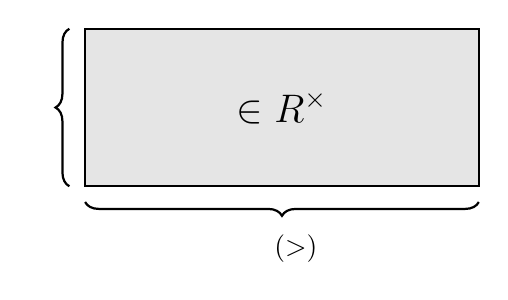
\begin{tikzpicture}
				\def\matHeight{2}
				\def\matWidth{5} 
				\draw[thick, fill=gray!20] (0,0) rectangle (\matWidth, \matHeight);
				\node at (0.5*\matWidth, 0.5*\matHeight) {\Large $\featuremtx \in \mathbb{R}^{\samplesize \times \nrfeatures}$};
				% vertical brace for samplesize (LEFT, correct orientation)
				\draw[decorate, decoration={brace, amplitude=5pt}, thick] 
  				(-0.2, 0) -- (-0.2, \matHeight)
  				node[midway, left=8pt] {$\samplesize$};
				\draw[decorate, decoration={brace, amplitude=5pt, mirror}, thick] 
        				(0, -0.2) -- (\matWidth, -0.2) 
        				node[midway, below=8pt] {$\nrfeatures \quad (\nrfeatures > \samplesize)$};
			\end{tikzpicture}
		\end{figure}
		See also: \gls{matrix}. },
	text={wide matrix}, 
	firstplural={wide matrices}, 
	plural={wide matrices}, 
	type=math,
   	first={wide matrix} 
}

\newglossaryentry{randomexperiment}
{name={random experiment},
	description={A random experiment\index{random experiment} is a physical (or abstract) process 
    	 	that produces an \gls{outcome} $\outcome$ from a set $\samplespace$ of possibilities. 
	 	This set of all possible \glspl{outcome} is referred to as the \gls{samplespace} of 
	 	the experiment. The key characteristic of a random experiment is that its 
	 	\gls{outcome} is unpredictable (or uncertain). Any measurement or observation 
	 	of the \gls{outcome} is an \gls{rv}, i.e., a \gls{function} of the \gls{outcome} $\outcome \in \samplespace$. 
	 	\Gls{probability} theory uses a \gls{probspace} as a mathematical structure for the study of 
	 	random experiments. A key conceptual property of a random experiment is that it can 
	 	be repeated under identical conditions. Strictly speaking, repeating a random experiment 
	 	a given number of $\samplesize$ times defines a new random experiment. The \glspl{outcome} 
	 	of this new experiment are length-$\samplesize$ \glspl{sequence} of \glspl{outcome} 
	 	from the original experiment (see Fig. \ref{fig_randomexperiment_dict}). While the \gls{outcome} of a single experiment is 
	 	uncertain, the long-run behaviour of the \glspl{outcome} of repeated experiments 
	 	tends to become increasingly predictable. This informal claim can be made 
	 	precise via fundamental results of \gls{probability} theory, such as the \gls{lln} 
	 	and the \gls{clt}.
	 	\begin{figure}[H]
		\begin{center}
	 		\begin{tikzpicture}[>=Stealth, node distance=1.5cm and 2cm, every node/.style={font=\small}]
			\node (experiment) [draw, rectangle, rounded corners, minimum width=2.6cm, align=center] {random\\experiment};
			\node (omega) [right=of experiment] {$\outcome \in \samplespace$};
			\coordinate (rightpad) at ($(omega.east) + (0.2,0)$);
			\draw[->] (experiment) -- (omega);
			\node (sequence) [below=of experiment, yshift=-0.5cm] {$(\outcome^{(1)}, \,\outcome^{(2)}, \,\dots, \,\outcome^{(\samplesize)})$};
			\node (sequence1) [below=of sequence, yshift=-0.5cm] {$(\datapoint^{(1)}, \,\datapoint^{(2)}, \,\dots, \,\datapoint^{(\samplesize)})$};
			\draw[->, thick] (experiment.south) -- node[midway, right, xshift=3pt] {repeat $\samplesize$ times} (sequence.north);
			\draw[->, thick] (sequence.south) -- node[midway, right, xshift=3pt] {\glspl{rv}} (sequence1.north);
			% Anchor node ~60% along the repeat arrow
			\path (experiment.south) -- (sequence.north) coordinate[pos=0.6] (repeatpoint);
			% Dotted rounded box enclosing experiment and part of repeat arrow
        			\node[draw=black, rounded corners, dotted, fit={(experiment) (repeatpoint) (rightpad)}, inner sep=8pt, label=above:{new random experiment with $\samplespace' = \samplespace \times \ldots \times \samplespace$}] {};
	 		\end{tikzpicture}
	     	\end{center}
		\caption{A random experiment produces an \gls{outcome} $\outcome \in \samplespace$ from a set 
			of possibilities (i.e., a \gls{samplespace}) 
			$\samplespace$. Repeating the experiment $\samplesize$ times yields another random 
			experiment, whose \glspl{outcome} are \glspl{sequence} 
			$(\outcome^{(1)}, \,\outcome^{(2)}, \,\dots, \,\outcome^{(\samplesize)}) \in \samplespace\times\ldots\times \samplespace$. 
			One example of a random experiment arising in many \gls{ml} applications is the gathering 
			of a \gls{trainset} $\datapoint^{(1)},\,\ldots,\,\datapoint^{(\samplesize)}$. \label{fig_randomexperiment_dict}}
	 	\end{figure} 
	 	Examples for random experiments arising in \gls{ml} applications include the following: 
	 	\begin{itemize} 
			\item \Gls{data} collection: The \glspl{datapoint} collected in \gls{erm}-based methods 
			can be interpreted as \glspl{rv}, i.e., as \glspl{function} of the \gls{outcome} $\outcome \in \samplespace$ 
			of a random experiment. 
			\item \Gls{stochGD} uses a random experiment at each iteration to select a subset of 
			the \gls{trainset}. 
			\item \Gls{privprot} methods use random experiments to perturb  
			the \glspl{output} of an \gls{ml} method to ensure \gls{diffpriv}. 
	 	\end{itemize} 
		See also: \gls{outcome}, \gls{samplespace}, \gls{rv}, \gls{probability}, \gls{probspace}.},
 	firstplural={random experiments},
 	plural={random experiments},
	type=math,
 	first={random experiment},
 	text={random experiment}
}

\newglossaryentry{pseudoinverse}
{name={pseudoinverse},
	description={The \index{pseudoinverse}Moore–Penrose pseudoinverse $\mA^{+}$ 
 		of a \gls{matrix} $\featuremtx \in \mathbb{R}^{\samplesize \times \nrfeatures}$ 
		generalizes the notion of an \gls{inverse} \cite{GolubVanLoanBook}. 
		The pseudoinverse arises naturally in \gls{ridgeregression} for a 
		\gls{dataset} with \gls{featuremtx} $\featuremtx$ and \gls{labelvec} 
		$\labelvec$ \cite[Ch.\ 3]{hastie01statisticallearning}. 
		The \glspl{modelparam} learned by \gls{ridgeregression} 
  		are given by
  		\[
  		\widehat{\weights}^{(\regparam)}  = \big(\featuremtx^{T} \featuremtx + \regparam \mI \big)^{-1} \featuremtx^{T} \vy, \quad \regparam > 0.
  		\]
  		We can then define the pseudoinverse $\featuremtx^{+} \in \mathbb{R}^{\nrfeatures \times \samplesize}$ via 
  		the limit \cite[Ch. 3]{benisrael2003generalized}
  		\[
  		\lim_{\regparam \to 0^+} \widehat{\weights}^{(\regparam)} = \featuremtx^+ \vy.
  		\]
		\\
		See also: \gls{matrix}, \gls{inverse}, \gls{ridgeregression}. },
 	first={pseudoinverse},
 	type=math, 
 	text={pseudoinverse}
} 

\newglossaryentry{tallmatrix}
{name={tall matrix},
	description={A\index{tall matrix} \gls{matrix} $\featuremtx \in \mathbb{R}^{\samplesize \times \nrfeatures}$ 
		is referred to as tall if it has more rows than columns, i.e., 
		when $\samplesize > \nrfeatures$.
		\begin{figure}[H]
			\centering
			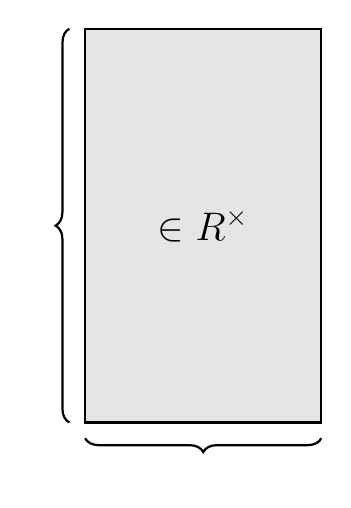
\begin{tikzpicture}
				\def\matHeight{5}
				\def\matWidth{3} 
				\draw[thick, fill=gray!20] (0,0) rectangle (\matWidth, \matHeight);
				\node at (0.5*\matWidth, 0.5*\matHeight) {\Large $\featuremtx \in \mathbb{R}^{\samplesize \times \nrfeatures}$};
				% vertical brace for samplesize (LEFT, correct orientation)
				\draw[decorate, decoration={brace, amplitude=5pt}, thick] 
  				(-0.2, 0) -- (-0.2, \matHeight)
  				node[midway, left=8pt] {$\samplesize$};
				\draw[decorate, decoration={brace, amplitude=5pt, mirror}, thick] 
        				(0, -0.2) -- (\matWidth, -0.2) 
        				node[midway, below=8pt] {$\nrfeatures$};
			\end{tikzpicture}
		\end{figure}
		See also: \gls{matrix}. },
	text={tall matrix}, 
	firstplural={tall matrices}, 
	plural={tall matrices}, 
	type=math,
   	first={tall matrix} 
}

\newglossaryentry{mgf}
{name={moment generating function (MGF)}, 
	description={Consider the\index{moment generating function (MGF)} MGF $\mgf{x}{t}$ 
	 	of a real-valued \gls{rv} $x$, which is defined as
	 	$\mgf{x}{t} = \expect \{ \exp(t \cdot x) \}$ for any $t \in \mathbb{R}$ 
	 	for which this \gls{expectation} exists \cite[Sec. 21]{BillingsleyProbMeasure}. 
		As its name indicates, the MGF allows us to compute the moments 
	 	$\expect\{ x^{k} \}$ for $k \in \mathbb{N}$. 
	 	In particular, the $k$th moment is obtained by evaluating the $k$th 
	 	derivative of $\mgf{x}{t}$ for $t=0$, i.e., $\expect\{ x^{k} \} = \mgfder{x}{k}{0}$. 
	 	This fact can be verified by the following identities: 
	 	\begin{align}
			\mgf{x}{t} & =\expect\{ \exp(t \cdot x)  \} \nonumber \\ 
			& \stackrel{(a)}{=} \expect\!\bigg\{\sum_{k=0}^{\infty} \frac{t^{k}}{k!} x^{k}\bigg\}  \nonumber \\ 
			& \stackrel{(b)}{=}  \sum_{k=0}^{\infty} \frac{t^{k}}{k!}\, \expect\!\big\{ x^{k} \big\}. \nonumber
	 	\end{align}
	 	Here, step $(a)$ is due to the Taylor series expansion of 
	 	$\exp\,(t \cdot x)$ and step $(b)$ is valid when the MGF exists 
	 	for all $t$ in some interval $(-t_{0},t_{0})$ \cite[p. 278]{BillingsleyProbMeasure}.
	 	\begin{figure}[H]
			\centering
			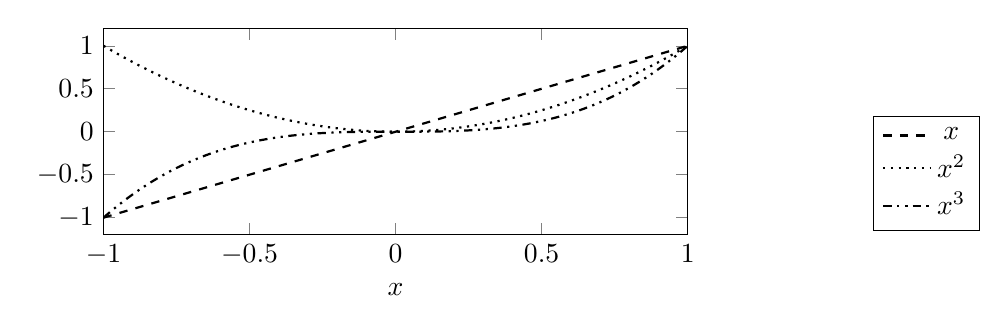
\begin{tikzpicture}
			\begin{axis}[
				width=9cm, height=4.2cm,
				domain=-1:1,
				samples=200,
				%axis lines*=left,        % removes bounding box, keeps left axis
				xlabel={$x$},
				ylabel={},
				ytick=\empty,
				ytick={-1,-0.5,0,0.5,1}, % manually set x-ticks
            			yticklabels={$-1$,$-0.5$,$0$,$0.5$,$1$},
				xtick={-1,-0.5,0,0.5,1}, % manually set x-ticks
            			xticklabels={$-1$,$-0.5$,$0$,$0.5$,$1$},
				xmin=-1, xmax=1,
				legend style={at={(1.5,0.02)},anchor=south east}
				]
				% f1 = x
				\addplot[thick, dashed] {x};
				\addlegendentry{$x$}
				% f2 = x^2
				\addplot[thick, dotted] {x^2};
				\addlegendentry{$x^{2}$}
				% f3 = x^3
				\addplot[thick, dashdotdotted] {x^3};
				\addlegendentry{$x^{3}$}
			\end{axis}
			\end{tikzpicture}
		\caption{The first few powers of an \gls{rv} $x$. The MGF 
			encodes the moments of $x$, which are the \glspl{expectation} 
			of the powers $x^{k}$ for $k=1,\,2,\,\ldots$.}
		\end{figure}
		The MGF is a useful tool for the study of sums of independent 
		\glspl{rv}. As a case in point, if $x$ and $y$ are independent 
		\glspl{rv}, then the MGF of their sum $z = x + y$ typically 
		satisfies $\mgf{z}{t} = \mgf{x}{t}\,\mgf{y}{t}$,
        		i.e., the MGF of the sum is typically the pointwise product of the 
		individual MGFs \cite[p.~280]{BillingsleyProbMeasure}.
		\\
 		See also: \gls{rv}, \gls{expectation}. }, 
 	first={moment generating function (MGF)}, 
 	firstplural={moment generating functions (MGFs)}, 
 	plural={MGFs}, 
 	type=math, 
 	text={MGF}
} 

\newglossaryentry{chernoffbound}
{name={Chernoff bound}, 
	description={The Chernoff bound\index{Chernoff bound} is a \gls{concentrationinequ} 
		derived as a direct application of \gls{markovsinequality} \cite[Ch.\ 2]{vershynin2018high}. 
		Let $\feature$ be a real-valued \gls{rv} such that its \gls{mgf} 
		$\mgf{\feature}{t}=\expect\{\exp\,(t x)\}$ exists for some $t>0$. 
		Applying \gls{markovsinequality} to the nonnegative 
		\gls{rv} $\exp\,(t \feature)$ yields, for any $\eta\in\mathbb{R}$, 
		\begin{equation}
			\prob{ \feature \ge \eta }
			= \prob{ \exp(t \feature) \ge \exp(t\eta)}
			\le \exp(-t\eta)\, \expect\{\exp\,(t \feature)\}\nonumber.
		\end{equation}
		Note that this is actually an entire family of upper bounds, parameterized 
		by all valid choices for $t>0$ (i.e., $\mgf{\feature}{t}$ must exist). 
		\\
		See also: \gls{concentrationinequ}, \gls{markovsinequality}, \gls{chebyshevsinequality}, 
		\gls{hoeffdingsinequality}.}, 
 	first={Chernoff bound}, 
 	type=math, 
 	text={Chernoff bound}
}

\newglossaryentry{rankdeficient}
{name={rank-deficient},
	description={A \gls{matrix} $\mA \in \mathbb{R}^{\samplesize \times \nrfeatures}$ 
         	is \gls{rank}-deficient\index{rank-deficient} if it is not \gls{fullrank}, i.e., 
         	when $\rank{\mA} < \min\{\samplesize,\nrfeatures\}$.
 		\begin{figure}[H]
			\begin{center}
			\begin{tikzpicture}[x=2cm]
				% LEFT: Standard basis vectors and unit square
				\begin{scope}
					\draw[->, thick] (0,0) -- (1,0) node[below] {$\vu^{(1)}$};
					\draw[->, thick] (0,0) -- (0,1) node[above] {$\vu^{(2)}$};
					%\draw[fill=gray!15] (0,0) -- (1,0) -- (1,1) -- (0,1) -- cycle;
					%\node at (0.5,0.5) {\small unit square};
					%\node at (0.5,-0.6) {standard basis};
				\end{scope}
				% RIGHT: Transformed basis vectors and parallelogram
				\begin{scope}[shift={(3.2,0)}]
				%\draw[->, thick] (0,0) -- (1,0) node[below] {$\vv^{(1)}$};
				%	\draw[->, thick] (0,0) -- (0,1) node[above] {$\vv^{(2)}$};
					\coordinate (A) at (0.2,0.0);
					\coordinate (B) at (2.0,0.0);
					\draw[->, very thick, red] (0,0) -- (A) node[below,yshift=-2pt] {$\mA \vu^{(1)}$};
					\draw[->, very thick, red] (0,0) -- (B) node[above,yshift=2pt] {$\mA \vu^{(2)}$};
					%	\node[blue] at (0.25,1.25) {};
					%	\node at (0.8,-0.6) {transformed basis};
				\end{scope}
				% Arrow between plots
				\draw[->, thick] (1.6,0.5) to[bend left] node[midway, above] {$\mA$} (2.7,0.5);
				%	\draw[->, thick] (1.3,0.5) -- (2.4,0.5) node[midway, above] {$\mA$};
			\end{tikzpicture}
			\end{center}
		\caption{Example of a \gls{rank}-deficient \gls{matrix} 
			$\mA \in \mathbb{R}^{2 \times 2}$.	\label{fig_matrix_rank_defdict}} 
		\end{figure} 
		In \gls{linreg}, the solution of the \gls{erm} problem is not 
		unique whenever the \gls{featuremtx} $\featuremtx$ is such that 
		the \gls{matrix} $\featuremtx^{\top}\featuremtx$ is \gls{rank}-deficient.
		\\
   		See also: \gls{fullrank}, \gls{dimension}, \gls{vectorspace}. }, 
	first={rank-deficient}, 
   	type=math,
   	text={rank-deficient}
}

\newglossaryentry{fullrank}
{name={full-rank},
 	description={A \gls{matrix} $\mA \in \mathbb{R}^{\samplesize \times \nrfeatures}$ 
  		is\index{full-rank} full-\gls{rank} if it has \gls{maximum} \gls{rank} \cite{StrangLinAlg2016}. 
  		For a \gls{tallmatrix}, i.e., when $\nrfeatures < \samplesize$, being 
  		full-\gls{rank} means that its \gls{rank} is equal to $\nrfeatures$. 
 		\begin{figure}[H]
			\centering
			\begin{tikzpicture}[every node/.style={font=\small}]
			% --- Full-rank square ---
			\node at (0,2) {$
			\mA =
			\begin{pmatrix}
			1 & 2\\
			3 & 4
			\end{pmatrix}
			$};
			\node[below=0.8cm of {$(0,2)$}] {\small full-\gls{rank} square};
			% --- Rank-deficient square ---
			\node at (4.5,2) {$
			\mB =
			\begin{pmatrix}
			1 & 2\\
			2 & 4
			\end{pmatrix}
			$};
			\node[below=0.8cm of {$(4.5,2)$}] {\small \gls{rankdeficient} square};
			% --- Full-rank tall (3x2) ---
			\node at (0,-1.0) {$
			\mC =
			\begin{pmatrix}
			1 & 0\\
			0 & 1\\
			1 & 1
			\end{pmatrix}
			$};
			\node[below=1.2cm of {$(0,-1.0)$}] {\small full-\gls{rank} \gls{tallmatrix}};
			% --- Rank-deficient wide (2x3) ---
			\node at (4.5,-1.0) {$
			\mD =
			\begin{pmatrix}
			1 & 2 & 3\\
			2 & 4 & 6
			\end{pmatrix}
			$};
			\node[below=1.2cm of {$(4.5,-1.0)$}] {\small \gls{rankdeficient} \gls{widematrix}};
			\end{tikzpicture}
		\caption{Examples of full-\gls{rank} and \gls{rankdeficient} \glspl{matrix}.}
		\end{figure} 
  		A square \gls{matrix} is full-\gls{rank} if and only if it is invertible. 
		\\ 
  		See also: \gls{matrix}, \gls{rank}, \gls{dimension}, \gls{linearmap}, \gls{columnspace}.}, 
	text = {full-rank}, 
  	type=math,
  	first={full-rank} 
 }

\newglossaryentry{rank}
{name={rank},
	description={The rank\index{rank} of a \gls{matrix} $\mA \in \mathbb{R}^{\samplesize \times \nrfeatures}$, 
 		denoted as $\rank{\mA}$, is the \gls{maximum} number of \gls{linearlyindep} columns 
 		of $\mA$ \cite{StrangLinAlg2016}. Equivalently, the rank can be defined as the 
 		\gls{dimension} of the \gls{columnspace} $\linspan{\mA} = \big\{ \mA \weights \mbox{ for some } 
 		\weights \in \mathbb{R}^{\nrfeatures} \big\}$. The rank of a \gls{matrix} 
 		$\mA \in \mathbb{R}^{\samplesize \times \nrfeatures}$ can neither exceed the 
 		number of rows nor the number of columns of $\mA$ \cite{Horn91}, \cite{MeyerMatrixAnalysis}, 
		i.e., $\rank{\mA} \leq \min \{ \samplesize, \nrfeatures \}$.  
		\\ 
 		See also: \gls{matrix}, \gls{dimension}, \gls{columnspace}, \gls{linearmap}.}, 
	text={rank}, 
	type=math,
	first={rank} 
}

\newglossaryentry{inverse}
{name={inverse matrix},
	description={An inverse \gls{matrix}\index{inverse matrix} $\mA^{-1}$ is defined for a 
 		square \gls{matrix} $\mA \in \mathbb{R}^{n \times n}$ that is of \gls{fullrank}, meaning its 
 		columns are linearly independent. In this case, $\mA$ is said to be invertible, 
 		and its inverse satisfies 
 		\[
 		\mA \mA^{-1} = \mA^{-1} \mA = \mI.
 		\]  	
     		A square \gls{matrix} is invertible if and only if its \gls{det} is nonzero. Inverse \glspl{matrix} are 
     		fundamental in solving systems of linear equations and in the closed-form solution of 
     		\gls{linreg} \cite{Strang2007}, \cite{Horn91}.  The concept of an inverse \gls{matrix} can be extended 
     		to \glspl{matrix} that are not square or do not have \gls{fullrank}. One may define a ``left inverse'' $\mB$ 
     		satisfying $\mB \mA = \mI$ or a ``right inverse'' $\mC$ satisfying $\mA \mC = \mI$. 
     		For general rectangular or singular \glspl{matrix}, the Moore–Penrose \gls{pseudoinverse}
     		$\mA^{+}$ provides a unified concept of a generalized inverse \gls{matrix} \cite{GolubVanLoanBook}.
 		 \begin{figure}[H]
 			\centering
 			\begin{tikzpicture}[x=2cm,y=2cm]
 			% LEFT: Standard basis
 			\begin{scope}
 				\draw[->, thick] (0,0) -- (1,0) node[below right] {$\vx$};
 				\draw[->, thick] (0,0) -- (0,1) node[above left] {$\vy$};
 			\end{scope}
 			% CENTER: Transformed basis (by A)
 			\begin{scope}[shift={(2.0,0)}]
 				\coordinate (A) at (1.5,0.5);
 				\coordinate (B) at (-0.2,1.2);
				\draw[->, very thick, red] (0,0) -- (A) node[pos=0.5, below right] {$\mA \vx$};
 				\draw[->, very thick, red] (0,0) -- (B) node[above right] {$\mA \vy$};
 			\end{scope}
 			% RIGHT: Inverse transformation
 			\begin{scope}[shift={(4.9,0)}]
 				\draw[->, very thick, blue] (0,0) -- (1,0) node[pos=0.5, below] {$\mA^{-1} (\mA \vx) = \vx$};
 				\draw[->, very thick, blue] (0,0) -- (0,1) node[above] {$\mA^{-1} (\mA \vy) = \vy$};
 			\end{scope}
 			% Curved arrows between stages
 			\draw[->, thick, bend left=20] (1.2,0.4) to node[above] {$\mA$} (1.8,0.4);
 			\draw[->, thick, bend left=20] (3.8,0.4) to node[below] {$\mA^{-1}$} (4.4,0.4);
 			\end{tikzpicture}
 		\caption{A \gls{matrix} $\mathbf{A}$ represents a linear transformation of $\mathbb{R}^{2}$. The inverse \gls{matrix} $\mathbf{A}^{-1}$ 
 			represents the inverse transformation. \label{fig_matrix_inverse_dict}} 
 		\end{figure}
		See also: \gls{matrix}, \gls{det}, \gls{linreg}, \gls{pseudoinverse}.},
	first={inverse matrix},
	type=math,
	text={inverse matrix}
}

\newglossaryentry{matrix}
{name={matrix},
	description={A matrix\index{matrix} of size $\samplesize \times \nrfeatures$ is a 2-D array of numbers, 
 		which is denoted by 
		$$
  		\mA = \begin{pmatrix}
   		A_{1,1} & A_{1,2} & \dots  & A_{1,\nrfeatures} \\
		A_{2,1} & A_{2,2} & \dots  & A_{2,\nrfeatures} \\
		\vdots  & \vdots  & \ddots & \vdots \\
		A_{\samplesize,1} & A_{\samplesize,2} & \dots  & A_{\samplesize,\nrfeatures}
		\end{pmatrix} \in \mathbb{R}^{\samplesize \times \nrfeatures}.
		$$
		Here, $A_{\sampleidx,\featureidx}$ denotes the matrix entry in the $\sampleidx$th row and the 
		$\featureidx$th column. Matrices are useful representations of various mathematical objects \cite{StrangLinAlg2016},
		including the following:
		\begin{itemize}
			\item Systems of linear equations: We can use a matrix to represent a system of linear equations 
			$$ \begin{pmatrix}
			A_{1,1} & A_{1,2} \\
			A_{2,1} & A_{2,2}
			\end{pmatrix}
			\begin{pmatrix}
				w_1 \\
				w_2
			\end{pmatrix}
			=\begin{pmatrix}
				y_1 \\
				y_2
			\end{pmatrix}
			\quad \text{ compactly as } \quad \mA \vw = \vy.
			$$
    			One important example of systems of linear equations is the optimality condition for the 
    			\glspl{modelparam} within \gls{linreg}. 
			\item \Glspl{linearmap}:
			Consider a $\nrfeatures$-dimensional \gls{vectorspace} $\mathcal{U}$ and a $\samplesize$-dimensional \gls{vectorspace} $\mathcal{V}$. 
			If we fix a \gls{basis} $\mathbf{u}^{(1)},\,\ldots,\,\mathbf{u}^{(\nrfeatures)}$ for $\mathcal{U}$ and a \gls{basis} $\mathbf{v}^{(1)},\,\ldots,\,\mathbf{v}^{(\samplesize)}$ 
			for $\mathcal{V}$, each matrix $\mA \in \mathbb{R}^{\samplesize \times \nrfeatures}$ naturally defines a 
			\gls{linearmap} $\alpha: \mathcal{U} \rightarrow \mathcal{V}$ (see Fig. \ref{fig_matrix_dict}) such that
   			$$\vu^{(\featureidx)} \mapsto \sum_{\sampleidx=1}^{\samplesize} A_{\sampleidx,\featureidx} \vv^{(\sampleidx)}.$$
			\item \Glspl{dataset}: We can use a matrix to represent a \gls{dataset}. Each row 
			corresponds to a single \gls{datapoint}, and each column corresponds to a specific 
			\gls{feature} or \gls{label} of a \gls{datapoint}. 
		\end{itemize}
		\begin{figure}[H]
		\begin{center}
		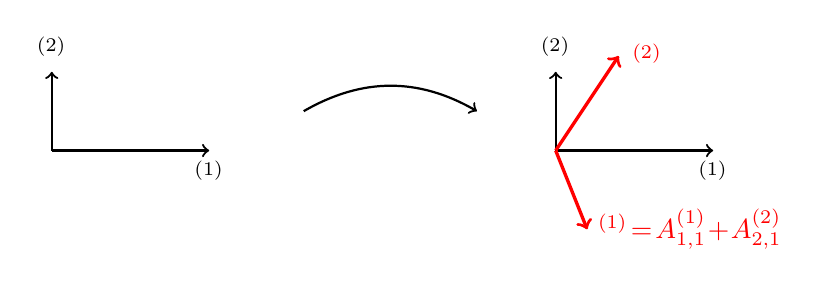
\begin{tikzpicture}[x=2cm]
			% LEFT: Standard basis vectors and unit square
			\begin{scope}
				\draw[->, thick] (0,0) -- (1,0) node[below] {$\vu^{(1)}$};
				\draw[->, thick] (0,0) -- (0,1) node[above] {$\vu^{(2)}$};
				%\draw[fill=gray!15] (0,0) -- (1,0) -- (1,1) -- (0,1) -- cycle;
				%\node at (0.5,0.5) {\small unit square};
				%\node at (0.5,-0.6) {standard basis};
			\end{scope}
			% RIGHT: Transformed basis vectors and parallelogram
			\begin{scope}[shift={(3.2,0)}]
				\draw[->, thick] (0,0) -- (1,0) node[below] {$\vv^{(1)}$};
				\draw[->, thick] (0,0) -- (0,1) node[above] {$\vv^{(2)}$};
				\coordinate (A) at (0.2,-1.0);
				\coordinate (B) at (0.4,1.2);
				\draw[->, very thick, red] (0,0) -- (A) node[below,right] {$\mA \vu^{(1)}\!=\!A_{1,1}\vv^{(1)}\!+\!A_{2,1}\vv^{(2)}$};
				\draw[->, very thick, red] (0,0) -- (B) node[right,xshift=1pt] {$\mA \vu^{(2)}$};
				%	\node[blue] at (0.25,1.25) {};
				%	\node at (0.8,-0.6) {transformed basis};
			\end{scope}
			% Arrow between plots
			\draw[->, thick] (1.6,0.5) to[bend left] node[midway, above] {$\mA$} (2.7,0.5);
		%	\draw[->, thick] (1.3,0.5) -- (2.4,0.5) node[midway, above] {$\mA$};
		\end{tikzpicture}
		\end{center}
		\caption{A matrix $\mA$ defines a \gls{linearmap} between two \glspl{vectorspace}. \label{fig_matrix_dict}} 
		\end{figure}
		See also: \gls{linearmap}, \gls{dataset}, \gls{linmodel}. },
	first={matrix},
	firstplural={matrices},
	type=math,
	plural={matrices},
	text={matrix}
}

\newglossaryentry{hyperplane}
{name={hyperplane},
	description={A hyperplane\index{hyperplane} is a $(\nrfeatures-1)$-dimensional affine 
		\gls{subspace} of a $\nrfeatures$-dimensional \gls{vectorspace}. In the 
		context of a \gls{euclidspace} $\mathbb{R}^{\nrfeatures}$, a 
		hyperplane is a set of the form
 		\[ 
		\{ \vx \in \mathbb{R}^\nrfeatures : \vw^\top \vx = b \}
  		\]
            where $\vw \in \mathbb{R}^d \setminus \{0\}$ is a normal \gls{vector} 
            and $b \in \mathbb{R}$ is an offset. Such a hyperplane  divides
            %partitions 
            %strictly speaking, this is not a partioning (e.g., exactly of the sets would need to include the boundary
		$\mathbb{R}^\nrfeatures$ into two \glspl{halfspace}
		\[\{ \vx \in \mathbb{R}^\nrfeatures : \vw^\top \vx > b \} \quad 
		\text{and} \quad \{ \vx \in \mathbb{R}^\nrfeatures : \vw^\top \vx > b \}.\]
 		Hyperplanes arise as the \glspl{decisionboundary} of \glspl{linclass}.
		\\
		See also: \gls{innerproduct}, \gls{subspace}, \gls{vectorspace}, \gls{euclidspace}, \gls{decisionboundary}. },
	first={hyperplane},
	type=math,
	plural={hyperplanes}, 
	firstplural={hyperplanes},
	text={hyperplane}
}

\newglossaryentry{normalvector}
{name={normal vector},
	description={See\index{normal vector} \gls{hyperplane}.},
	first={normal vector},
	type=math,
	plural={normal vectors}, 
	firstplural={normal vectors},
	text={normal vector}
}

\newglossaryentry{halfspace}
{name={halfspace},
	description={See\index{halfspace} \gls{hyperplane}.},
	first={halfspace},
	type=math,
	plural={halfspaces}, 
	firstplural={halfspaces},
	text={halfspace}
}

\newglossaryentry{subspace}
{name={subspace},
	description={A subset of a \gls{vectorspace} $\mathcal{V}$ is a subspace\index{subspace} of $\mathcal{V}$ if it is also a 
		\gls{vectorspace} with respect to the same operations as $\mathcal{V}$.
			   \\
		See also: \gls{vectorspace}.},
	type=math, 
	first={subspace},
	text={subspace}
}

\newglossaryentry{columnspace}
{name={column space},
	description={The column space\index{column space} of a \gls{matrix} 
		$\mA \in \mathbb{R}^{\samplesize \times \nrfeatures}$,
		denoted by $\linspan{\mA}$, is the set of all linear combinations of the 
		columns of $\mA$. In other words, 
		$$ \linspan{\mA} = \{ \mA \weights : \weights \in \mathbb{R}^{\nrfeatures} \}. $$
		The column space $\linspan{\mA}$ of the \gls{matrix} $\mA$ 
		is a \gls{subspace} of the \gls{euclidspace} $\mathbb{R}^{\samplesize}$.
			   \\
		See also: \gls{matrix}, \gls{vectorspace}.},
	type=math,
	first={column space},
	text={column space}
}

\newglossaryentry{mvndist}
{name={multivariate normal distribution}, 
	description={The\index{multivariate normal distribution} multivariate normal distribution, 
		which is denoted by $\mvnormal{\meanvecgeneric}{\covmtxgeneric}$, is a fundamental 
		\gls{probmodel} for numerical \glspl{featurevec} of fixed dimension $\nrfeatures$. 
		It defines a family of \glspl{probdist} over \gls{vector}-valued \glspl{rv} 
		$\featurevec \in \mathbb{R}^{\nrfeatures}$~\cite{BertsekasProb}, \cite{GrayProbBook}, \cite{Lapidoth09}. 
		Each distribution in this family is fully specified by its \gls{mean} \gls{vector} 
		$\meanvecgeneric \in \mathbb{R}^{\nrfeatures}$ and \gls{covmtx} 
		$\covmtxgeneric \in \mathbb{R}^{\nrfeatures \times \nrfeatures}$. When the 
		\gls{covmtx} $\covmtxgeneric$ is invertible, the corresponding \gls{probdist} is 
		characterized by the following \gls{pdf}:
		\[p(\featurevec) = 
 		\frac{1}{\sqrt{(2\pi)^{\nrfeatures} \det\,(\covmtxgeneric)}} 
 		\exp\left[ -\frac{1}{2} 
 		(\featurevec - \meanvecgeneric)\,^{T}\, \covmtxgeneric^{-1} 
 		(\featurevec - \meanvecgeneric) \right].
 		\]
		Note that this \gls{pdf} is only defined when $\covmtxgeneric$ is invertible.
   		More generally, any \gls{rv} $\featurevec \sim \mvnormal{\meanvecgeneric}{\covmtxgeneric}$ 
   		admits the following representation:
  		\[
    		\featurevec = \mA \vz + \meanvecgeneric
   		\]
   		where $\vz \sim \mvnormal{\mathbf{0}}{\mathbf{I}}$ is a \gls{stdnormvec} 
   		and $\mA \in \mathbb{R}^{\nrfeatures \times \nrfeatures}$ satisfies $\mA \mA^\top = \covmtxgeneric$. 
   		This representation remains valid even when $\covmtxgeneric$ is singular, in which case $\mA$ 
   		is not \gls{fullrank}~\cite[Ch. 23]{Lapidoth2017}.
   		The family of multivariate normal distributions is exceptional among \glspl{probmodel} for numerical 
   		quantities, at least for the following reasons. First, the family is closed under affine 
   		transformations, i.e.,
		\[ 
		\featurevec \sim \mathcal{N}(\meanvecgeneric,\covmtxgeneric) \mbox{ implies } 
		\mB\featurevec\!+\!\vc \sim \mathcal{N}\big( \mB\meanvecgeneric+\vc,\mB \covmtxgeneric \mB\,^{T} \big). 
		\]
		Second, the \gls{probdist} $\mathcal{N}(\mathbf{0},\covmtxgeneric)$ maximizes the 
		\gls{diffentropy} among all distributions with the same \gls{covmtx} $\covmtxgeneric$~\cite{coverthomas}. 
		\\ 
		See also: \gls{probmodel}, \gls{probdist}, \gls{stdnormvec}, \gls{diffentropy}, \gls{gaussrv}.}, 
	first={multivariate normal distribution},
	type=math, 
	text={multivariate normal distribution}
}

\newglossaryentry{stdnormvec}
{name={standard normal random vector}, 
	description={A\index{standard normal random vector} standard normal random \gls{vector} 
		is an \gls{rv} $\featurevec=\big(\feature_{1}, \,\ldots, \,\feature_{\nrfeatures}\big)\,^{T}$ 
		whose entries are \gls{iid} \glspl{gaussrv} $x_{\featureidx} \sim \mathcal{N}(0,1)$. 
		The \gls{probdist} of a standard normal random \gls{vector} is a special case 
		of a \gls{mvndist} $\featurevec \sim \mathcal{N}(\mathbf{0},\mathbf{I})$.
		\\ 
		See also: \gls{vector}, \gls{iid}, \gls{gaussrv}, \gls{mvndist}, \gls{rv}.}, 
	first={standard normal random vector},
	type=math, 
	text={standard normal random vector}
}

\newglossaryentry{continuous}
% This is perfectly fine, of course, to give the epsilon-delta-definition of continuity. The (equivalent) definition using  
% limits is perhaps though easier to understand, so it could be an alternative and could at least be briefly mentioned - 
% but  of course, just a remark, perfectly fine as it is.
{name={continuous}, 
	description={A \gls{function}\index{continuous} $f: \mathbb{R}^{\nrfeatures} \to \mathbb{R}$ is 
		continuous at a point $\featurevec' \in \mathbb{R}^{\nrfeatures}$ if, for 
	 	every $\epsilon > 0$, there is a $\delta > 0$ such that, for all 
	 	$\featurevec \in \mathbb{R}^{\nrfeatures}$ with $\normgeneric{\featurevec - \featurevec'}{2} < \delta$, 
	 	it holds that $|f(\featurevec) - f(\featurevec')| < \epsilon$ \cite{RudinBookPrinciplesMatheAnalysis}. 
	 	In other words, we can make $f(\featurevec)$ arbitrarily close to $f(\featurevec')$ 
	 	by choosing $\featurevec$ sufficiently close to $\featurevec'$. 
		\begin{figure}[H]
			\centering
	 		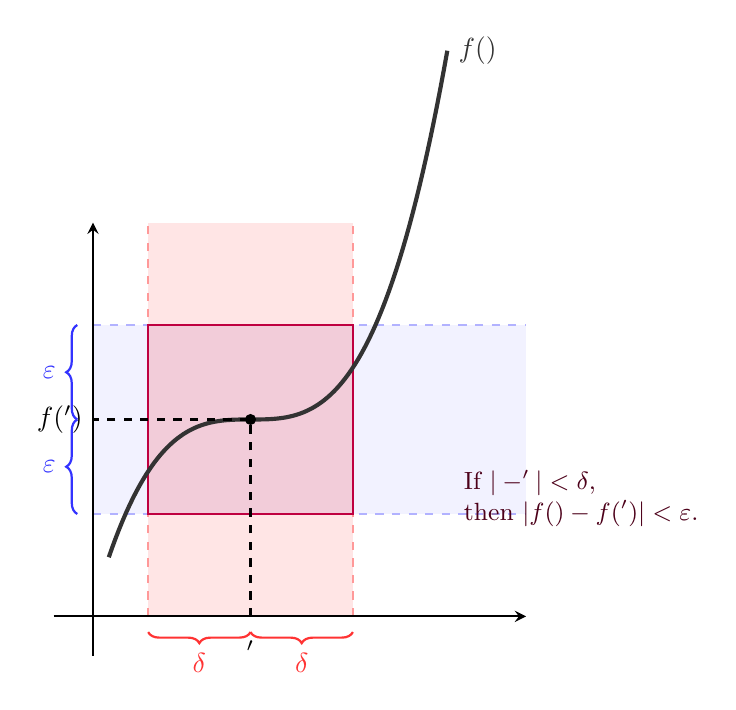
\begin{tikzpicture}[
				>=stealth, 
    				thick,
				%f(x) = 0.5(x-2)^3 + 2
    				declare function={f(\x) = 0.3*(\x-2)^3 + 2.5;}
				]
				\def\xprime{2}      % x'
    				\def\epsilonval{1.2}   % epsilon
				\def\deltaval{1.3}     % delta
				\def\xmax{5.5}
				\def\ymax{5}
				\fill[blue!5] (0, {f(\xprime)-\epsilonval}) rectangle (\xmax, {f(\xprime)+\epsilonval});
				\draw[blue!30, dashed] (0, {f(\xprime)-\epsilonval}) -- (\xmax, {f(\xprime)-\epsilonval});
				\draw[blue!30, dashed] (0, {f(\xprime)+\epsilonval}) -- (\xmax, {f(\xprime)+\epsilonval});
				\fill[red!10] ({\xprime-\deltaval}, 0) rectangle ({\xprime+\deltaval}, \ymax);
				\draw[red!40, dashed] ({\xprime-\deltaval}, 0) -- ({\xprime-\deltaval}, \ymax);
				\draw[red!40, dashed] ({\xprime+\deltaval}, 0) -- ({\xprime+\deltaval}, \ymax);
				\fill[purple!20] ({\xprime-\deltaval}, {f(\xprime)-\epsilonval}) rectangle ({\xprime+\deltaval}, {f(\xprime)+\epsilonval});
				\draw[purple, thick] ({\xprime-\deltaval}, {f(\xprime)-\epsilonval}) rectangle ({\xprime+\deltaval}, {f(\xprime)+\epsilonval});
				\draw[->] (-0.5,0) -- (\xmax,0) node[right] {$\feature$};
				\draw[->] (0,-0.5) -- (0,\ymax) node[above] {};
				% The Function 
				\draw[line width=1.5pt, black!80] plot[domain=0.2:4.5, samples=100] (\x, {f(\x)}) 
				node[right] {$f(\feature)$};
				\draw[dashed] (\xprime, 0) -- (\xprime, {f(\xprime)}) -- (0, {f(\xprime)});
				\fill[black] (\xprime, {f(\xprime)}) circle (2pt);
				\node[below,yshift=-5pt] at (\xprime, 0) {$\feature'$};
				\node[left] at (0, {f(\xprime)}) {$f(\feature')$};
				\draw[decorate, decoration={brace, amplitude=4pt}, blue!80] 
				(-0.2, {f(\xprime)}) -- (-0.2, {f(\xprime)+\epsilonval}) 
				node[midway, left=4pt] {$\varepsilon$};
				\draw[decorate, decoration={brace, amplitude=4pt}, blue!80] 
				(-0.2, {f(\xprime)-\epsilonval}) -- (-0.2, {f(\xprime)}) 
				node[midway, left=4pt] {$\varepsilon$};
				\draw[decorate, decoration={brace, amplitude=4pt, mirror}, red!80] 
				(\xprime, -0.2) -- ({\xprime+\deltaval}, -0.2) 
				node[midway, below=4pt] {$\delta$};
				\draw[decorate, decoration={brace, amplitude=4pt, mirror}, red!80] 
				({\xprime-\deltaval}, -0.2) -- (\xprime, -0.2) 
				node[midway, below=4pt] {$\delta$};
				\node[align=left, purple!40!black, font=\small] at (6.2, 1.5) 
				{If $| \feature - \feature' | < \delta$,\\
				then $| f(\feature) - f(\feature') | < \varepsilon$.};
			\end{tikzpicture}
		\caption{The \gls{function} $f(\feature) = 0.3(\feature-2)^3 + 2.5$ is continuous 
		         at every $\feature'$.}
		\end{figure}
		If $f$ is continuous at every point $\featurevec' \in \mathbb{R}^{\nrfeatures}$, then $f$ is said to be 
	 	continuous on $\mathbb{R}^{\nrfeatures}$. The notion of a continuous 
	 	\gls{function} can be naturally extended to \glspl{function} between general \glspl{metricspace} 
		\cite{RudinBookPrinciplesMatheAnalysis}.
		\\
		See also: \gls{euclidspace}, \gls{metric}.},
	first={continuous},
	type=math,
	text={continuous}
}

\newglossaryentry{minimum}
{name={minimum},
	description={Given a set of real numbers, the minimum\index{minimum} is the smallest of those numbers.
		Note that for some sets, such as the set of negative real numbers, the minimum does not exist.},
	firstplural={minima}, 
 	plural={minima},
	type=math, 
	first={minimum},
	text={minimum}
}

\newglossaryentry{co-domain}
{name={co-domain}, 
	description={The co-\gls{domain}\index{co-domain} of a \gls{function} 
		$f: \mathcal{U} \rightarrow \mathcal{V}$ is the set $\mathcal{V}$ 
		into which $f$ maps elements of its \gls{domain} $\mathcal{U}$.  
		\begin{figure}[H]
			\centering
			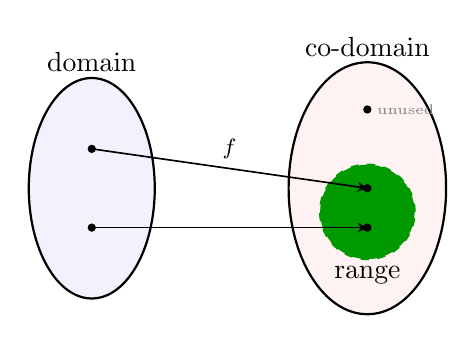
\begin{tikzpicture}[
			>=stealth, 
			node distance=2cm,
			scale=1.0, every node/.style={transform shape} % Scales the whole diagram down slightly
			]
			% Domain A
			\draw[thick, fill=blue!5] (0,0) ellipse (0.8cm and 1.4cm);
			\node[] at (0, 1.6) {\gls{domain}};
			% Codomain B
			\draw[thick, fill=red!5] (3.5,0) ellipse (1cm and 1.6cm);
			\node[] at (3.5, 1.8) {co-\gls{domain}};
			\draw[dashed, fill=green!10, thick, green!60!black] (3.5, -0.3) circle (0.6cm);
			\node[] at (3.5, -1.1) {range};
			\fill (0, 0.5) circle (1.5pt) coordinate (a1);
			\fill (0, -0.5) circle (1.5pt) coordinate (a2);
			% Output points
			\fill (3.5, 0) circle (1.5pt) coordinate (b1);
			\fill (3.5, -0.5) circle (1.5pt) coordinate (b2);
			% Unreached point
			\fill (3.5, 1.0) circle (1.5pt) coordinate (b_miss) node[right, font=\tiny, gray] {unused};
			\draw[->, semithick] (a1) -- (b1);
			\draw[->, semithick] (a2) -- (b2);
			% Function Label
			\node[font=\footnotesize] at (1.75, 0.5) {$f$};
			\end{tikzpicture}
		\end{figure}
		See also: \gls{domain}, \gls{function}, \gls{map}.},
	first={co-domain},
	firstplural={co-domains}, 
	type=math, 
	plural={co-domains},
	text={co-domain}
}

\newglossaryentry{cdf}
{name={cumulative distribution function (cdf)},
	description={The \index{cumulative distribution function (cdf)} cdf 
		$\cdf{\feature}{\eta}$ of a real-valued \gls{rv} $\feature$ is \cite{AshProbMeasure}, \cite{papoulis}
		$$\cdf{\feature}{\eta} \defeq \prob{\feature \leq \eta}.$$
					\\ 
		See also: \gls{rv}, \gls{pdf}, \gls{probdist}.},
	first={cumulative distribution function (cdf)},
	firstplural={cumulative distribution functions (cdfs)}, 
	plural={cdfs}, 
	type=math,
	text={cdf} 
}

\newglossaryentry{weightedgraph}
{name={weighted graph},
	description={A weighted \gls{graph} is a \gls{graph}\index{weighted graph} whose edges 
		are assigned numeric weights. Typically, these \glspl{edgeweight} 
		are nonnegative real numbers. For example, if a \gls{graph} represents 
		a road network with nodes corresponding to intersections and edges representing 
		road segments, the \gls{edgeweight} could represent the capacity (measured 
		in \gls{maximum} vehicles per hour) of the road segment \cite{NewmannBook}.  
		\begin{figure}[H] 
			\centering
			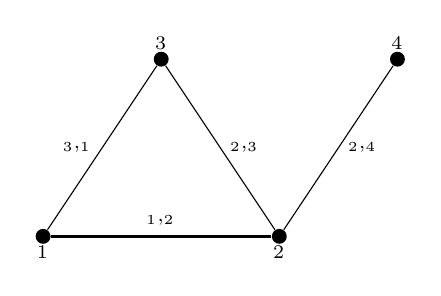
\begin{tikzpicture}[scale=1.5,
				node/.style={circle, fill=black, inner sep=1.9pt},
				lab/.style={anchor=west, xshift=3pt}
				]
				% Nodes (points)
				\node[node] (v1) at (0,0) {};
				\node[node] (v2) at (2,0) {};
				\node[node] (v3) at (1,1.5) {};
				\node[node] (v4) at (3,1.5) {};
				% Labels
				\node[anchor=north] at (v1) {$\nodeidx_1$};
				\node[anchor=north] at (v2) {$\nodeidx_2$};
				\node[anchor=south] at (v3) {$\nodeidx_3$};
				\node[anchor=south] at (v4) {$\nodeidx_4$};
				% Undirected edges
				\draw [line width=1pt] (v1) -- node[midway, above] {$\edgeweight_{\nodeidx_1,\nodeidx_2}$} (v2);
				\draw (v2) -- node[midway, right] {$\edgeweight_{\nodeidx_2,\nodeidx_3}$} (v3);
				\draw (v3) -- node[midway, left] {$\edgeweight_{\nodeidx_3,\nodeidx_1}$} (v1);
				\draw (v2) -- node[midway, right] {$\edgeweight_{\nodeidx_2,\nodeidx_4}$} (v4);
			\end{tikzpicture}
		\caption{A weighted \gls{graph} with four nodes 
			$\nodes = \{\nodeidx_1, \nodeidx_2, \nodeidx_3, \nodeidx_4\}$ 
			and four edges $\edges = \{\{\nodeidx_1,\nodeidx_2\},
			\{\nodeidx_2,\nodeidx_3\}, \{\nodeidx_3,\nodeidx_1\}, 
			\{\nodeidx_2,\nodeidx_4\}\}$. Each edge is assigned a weight.}
		\end{figure}		
		See also: \gls{graph}.},
	first={weighted graph},
	type=math,
	firstplural={weighted graphs}, 
	plural={weighted graphs}, 
	text={weighted graph} 
}

\newglossaryentry{graph}
{name={graph},
	description={A graph\index{graph} $\graph = \pair{\nodes}{\edges}$ 
		consists of a node set $\nodes$ and an edge set $\edges$.
		Each edge $\edgeidx \in \edges$ is characterized by the nodes to which 
		it is \gls{connected} and in what precise sense. For example, 
		an edge of a \gls{directedgraph} is leaving one node 
		and pointing to another node. An edge of an \gls{undirectedgraph} 
		connects two nodes without any sense of 
		direction \cite{NewmannBook}, \cite{RockNetworks}. 
		In principle, there can also be several (parallel) edges that are 
		\gls{connected} to the same nodes in the same way \cite{RockNetworks}. 
		Moreover, edges may connect a node to itself, resulting in 
		so-called self-loops \cite{NewmannBook}. 
		A simple \gls{undirectedgraph} contains no 
		parallel edges and no self-loops \cite{WilsonGraph2010}. 
		Each edge $\edgeidx \in \edges$ of a simple \gls{undirectedgraph}
		can be identified with a set of two nodes ${\nodeidx,\nodeidx'}$. 
		\begin{figure}[H] 
			\centering
			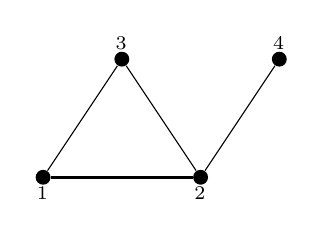
\begin{tikzpicture}[scale=1,
				node/.style={circle, fill=black, inner sep=1.9pt},
				lab/.style={anchor=west, xshift=3pt}
				]
				% Nodes (points)
				\node[node] (v1) at (0,0) {};
				\node[node] (v2) at (2,0) {};
				\node[node] (v3) at (1,1.5) {};
				\node[node] (v4) at (3,1.5) {};
				% Labels
				\node[anchor=north] at (v1) {$\nodeidx_1$};
				\node[anchor=north] at (v2) {$\nodeidx_2$};
				\node[anchor=south] at (v3) {$\nodeidx_3$};
				\node[anchor=south] at (v4) {$\nodeidx_4$};
				% Undirected edges
				\draw [line width=1pt] (v1) -- (v2);
				\draw (v2) -- (v3);
				\draw (v3) -- (v1);
				\draw (v2) -- (v4);
			\end{tikzpicture}
		\caption{A simple \gls{undirectedgraph} with four nodes 
			$\nodes = \{\nodeidx_1, \nodeidx_2, \nodeidx_3, \nodeidx_4\}$ 
			and four edges $\edges = \{\{\nodeidx_1,\nodeidx_2\},
			\{\nodeidx_2,\nodeidx_3\}, \{\nodeidx_3,\nodeidx_1\}, 
			\{\nodeidx_2,\nodeidx_4\}\}$.}
		\end{figure}
		\Glspl{weightedgraph} assign a numerical value $\edgeweight_{\edgeidx}$, 
		referred to as \gls{edgeweight}, to each edge $\edgeidx \in \edges$.
					\\ 
		See also: \gls{map}, \gls{edgeweight}.},
 	first={graph},
 	text={graph}, 
 	firstplural={graphs}, 
	plural={graphs}, 
 	type=math
}

\newglossaryentry{markovchain}
{name={Markov chain},
	description={A Markov chain\index{Markov chain} is a \gls{stochproc} $\{X_\timeidx \}_{\timeidx \in \mathbb{N}}$ 
		defined on a common \gls{probspace} and using the index set $\mathbb{N}$. The 
		\gls{rv} $X_\timeidx$ might represent (the generation of) a state of a physical system 
		at the time instant $\timeidx$. The defining property of a Markov chain 
		is the \gls{markovprop} \cite{durrett2010probability}, \cite{papoulis}, \cite{NorrisMarkovChains1997}.
		For all $\timeidx \in \mathbb{N}$,
 		\begin{equation}
 			\nonumber \probdist^{(X_{\timeidx+1} \mid X_\timeidx,\ldots,X_1)} = \probdist^{(X_{\timeidx+1} \mid X_\timeidx)}. 
 		\end{equation}
 		In other words, the \gls{condprobdist} of the next state $X_{\timeidx+1}$ 
		depends on the past $X_{\timeidx},X_{\timeidx-1},\,\dots,\,X_{1}$ 
		only through the current state $X_{\timeidx}$. The concept of a 
		Markov chain can be generalized from discrete time (with index set $\mathbb{N}$) 
		to continuous time (with index set $\mathbb{R}$) \cite{NorrisMarkovChains1997}. 
		\\ 
		See also: \gls{stochproc}, \gls{mdp}, \gls{condprobdist}.},
	first={Markov chain},
	type=math,
    	text={Markov chain}, 
	plural={Markov chains}, 
	firstplural={Markov chains}
}

\newglossaryentry{markovprop}
{name={Markov property},
	description={See \gls{markovchain}\index{Markov property}.},
	first={Markov property},
	type=math,
	text={Markov property}
}

\newglossaryentry{em}
{name={expectation–maximization (EM)}, 
	description={\index{expectation–maximization (EM)}
	    	The EM \gls{algorithm} \cite{dempster1977maximum} is an iterative \gls{optmethod} for 
		approximately solving certain \gls{maxlikelihood} \glspl{optproblem} 
		that are difficult to solve directly \cite[Sec. 9.4]{BishopBook}, \cite[Sec. 11.4.7]{Murphy2012}.
	    	To motivate the EM \gls{algorithm} and explain its construction, 
		consider an \gls{ml} application involving a single observed \gls{datapoint} 
		with \gls{feature} $\feature \in \featurespace$, where $\featurespace$ 
		is a finite \gls{featurespace}. The \gls{data} generation 
		is modeled via a \gls{probmodel} that consists of an \gls{rv} $\feature'$ 
		with \gls{pmf} $\pmf{\feature'}{\cdot;\weights}$. Here, 
		the actual \glspl{modelparam} $\weights \in \paramspace$—used for the \gls{data} 
		generation via sampling from $\pmf{\feature'}{\cdot;\weights}$—are unknown. A widely 
		used approach for estimating these \glspl{modelparam} is via the solutions of the \gls{maxlikelihood} 
		problem
		\begin{equation}
			\label{equ_def_ML_EM_dict}
			\min_{\weights \in \paramspace} - \log \pmf{\feature'}{\feature;\weights}.
		\end{equation}
		For some \glspl{probmodel}, such as a \gls{gmm}, this \gls{optproblem} can be 
		difficult to solve directly. As a work-around, one can often introduce an auxiliary 
		attribute $\truelabel \in \labelspace$, generated via some \gls{rv} $\truelabel'$, 
		such that the corresponding \gls{probmodel} $\pmf{\feature',\truelabel'}{\cdot,\cdot;\weights}$ 
		yields a much easier \gls{maxlikelihood} problem 
		\begin{equation}
			\label{equ_def_complete_EM_dict}
			\min_{\weights \in \paramspace} 
			- \log \pmf{\feature',\truelabel'}{\feature,\truelabel;\weights}.
		\end{equation}
		The attribute $\truelabel$ is introduced solely to simplify 
		\eqref{equ_def_complete_EM_dict}, but it is not observed in practice—only the 
		feature $\feature$ is available. Thus, we cannot solve \eqref{equ_def_complete_EM_dict} 
		directly as we do not know which value $\truelabel$ to plug into the \gls{pmf} 
		$ \pmf{\feature',\truelabel'}{\feature,\truelabel;\weights}$. 
		The EM method resolves this dilemma by alternating between the following two steps:
		1) an E-step, in which a “soft’’ estimate of the auxiliary attribute $\truelabel$ is computed 
		in the form of the \gls{posterior} $\pmf{\truelabel'|\feature'}{\cdot;\widehat{\weights}}$
		using the current choice $\widehat{\weights}$ for the \glspl{modelparam}; and 
		2) an M-step, in which a surrogate \gls{objfunc} derived from this \gls{posterior} is minimized.
		The completion of these two steps constitutes one full \gls{iteration} of 
		the EM method. 
		In more detail, the E-step produces the \gls{function}
		\[
		Q(\weights \mid \widehat{\weights})
		\defeq 
		- \sum_{\truelabel \in \labelspace} 
		\pmf{\truelabel'|\feature'}{\truelabel;\widehat{\weights}}
		\log\!\Big(
		\pmf{\feature',\truelabel'}{\feature,\truelabel;\weights}
		/\pmf{\truelabel'|\feature'}{\truelabel;\widehat{\weights}}
		\Big)
		\]
		and the M-step minimizes $Q(\weights \mid \widehat{\weights})$ over 
		$\weights \in \paramspace$.
		This \gls{function} satisfies the following two key properties 
		\cite[Sec. 9.4]{BishopBook},\cite[Sec. 11.4.7]{Murphy2012}:
		1) upper bound
		$Q(\weights\mid \widehat{\weights})
		\geq
		- \log \pmf{\feature'}{\feature;\weights}$,
		for all $\weights \in \paramspace$;
		and 2) tightness
		$Q(\widehat{\weights}\mid \widehat{\weights})
		=- \log \pmf{\feature'}{\feature;\widehat{\weights}}.$
		To summarize, during each \gls{iteration}, EM minimizes an upper-bounding 
		surrogate \gls{objfunc} that is tight at the current iterate $\widehat{\weights}$. 
		Thus, EM is a \gls{majmin} method for approximately solving \eqref{equ_def_ML_EM_dict}. 
		The above construction and analysis of EM can be extended to more 
		general settings involving multiple \glspl{datapoint} 
		and infinite \glspl{featurespace} such as $\mathbb{R}^{\featuredim}$ 
		(see \cite[Sec. 11.4.7]{Murphy2012} for further details). 
			\\
		See also: \gls{maxlikelihood}, \gls{optproblem}, \gls{probmodel}. },
	first={expectation–maximization (EM)},
	type=math, 
	text={EM}
}

\newglossaryentry{ppca}
{name={probabilistic principal component analysis (PPCA)}, 
	description={PPCA\index{probabilistic principal component analysis (PPCA)} 
		extends basic \gls{pca} by using a \gls{probmodel} for \glspl{datapoint}. 
		Using a \gls{probmodel} allows to cast \gls{dimred} as an estimation problem 
		that can be solved using \gls{em} \cite{TippingProbPCA}.
				\\
		See also: \gls{pca}, \gls{probmodel}, \gls{dimred}, \gls{em}.},
	first={probabilistic principal component analysis (PPCA)},
	type=math, 
	text={PPCA}
}

\newglossaryentry{contractop}
{name={contractive operator},
	description={An\index{contractive operator} \gls{operator} 
		$\fixedpointop: \mathbb{R}^{\nrfeatures} \rightarrow \mathbb{R}^{\nrfeatures}$
		is a contraction (or contractive) if, for some $\contractfac \in [0,1)$, 
 	   	\cite{BausckeCombette}, \cite{ProximalMethods}
		\begin{equation} 
			\nonumber
			\normgeneric{ \fixedpointop \weights\!-\!\fixedpointop \weights'}{2}  \leq 
			 \contractfac	\normgeneric{\weights\!-\!\weights'}{2} \mbox{ holds for any } \weights,\weights' \in \mathbb{R}^{\nrfeatures}.
		\end{equation} 
		The notion of a contractive \gls{operator} generalizes naturally from $\mathbb{R}^{\nrfeatures}$ 
		to arbitrary \glspl{metricspace} \cite{BausckeCombette}.
		\begin{figure}[H]
    			\centering
    			\begin{tikzpicture}[>=Latex, font=\small]
        			% Styles
        			\tikzset{
            		space/.style={draw, thick, circle, minimum size=4.0cm},
            		pt/.style={circle, inner sep=1.5pt, draw, fill=black},
            		maparrow/.style={->, very thick},
            		distline/.style={dashed, thick}
        			}
        			% Single space
        			\node[space,label=above:{$\featurespace$}] (X) at (0,0) {};
        			% Two points and their images under T inside the same space
        			\coordinate (x1)  at (-1.0,0.8);
        			\coordinate (x2)  at ( 1.0,0.8);
        			\coordinate (Tx1) at (-0.5,0.1);
        			\coordinate (Tx2) at ( 0.5,0.1);
        			% Points x, x'
        			\node[pt,label=above left:{$\featurevec$}] at (x1) {};
        			\node[pt,label=above right:{$\featurevec'$}] at (x2) {};
        			% Images T(x), T(x')
        			\node[pt] (TX1) at (Tx1) {};
        			\node[pt] (TX2) at (Tx2) {};
        			\node[anchor=east] at ($(TX1.west)+(-4pt,-2pt)$) {$\fixedpointop \featurevec$};
        			\node[anchor=west] at ($(TX2.east)+(4pt,-2pt)$) {$\fixedpointop \featurevec'$};
        			% Contraction effect: distances shrink
        			\draw[distline] (x1) -- (x2)
            		node[midway, above=4pt] {$\metric{\featurevec}{\featurevec'}$};
        			\draw[distline] (Tx1) -- (Tx2)
            		node[midway, below=4pt] {$\metric{\fixedpointop \featurevec}{\fixedpointop \featurevec'}$};
        			% Fixed point in the same space
        			\coordinate (xs) at (0,-0.9);
        			\node[pt,label=below:{$\featurevec^\star$}] (XS) at (xs) {};
        			% Small loop indicating T(x*) = x*
        			%\draw[maparrow,shorten >=2pt,shorten <=2pt]
            		%(XS) .. controls +(60:0.7) and +(120:0.7) .. (XS);
        			\node at (0,-1.6) {$\fixedpointop \featurevec^\star = \featurevec^\star$};
    			\end{tikzpicture}
    		\caption{A contractive \gls{operator} $\fixedpointop:\featurespace\to\featurespace$ 
      			has a unique fixed point $\featurevec^\star$ with $\fixedpointop \featurevec^\star=\featurevec^\star$.
      			For any two points $\featurevec,\featurevec'$ in the same space, the distance between their images
      			$\fixedpointop\featurevec$ and $\fixedpointop\featurevec'$ is strictly smaller.}
    			\label{fig:contract_dict}
		\end{figure}
		Intuitively, a contractive \gls{operator} brings any two points 
		from its \gls{domain} closer together by at least a factor of $\contractfac$.
		\\ 
		See also: \gls{operator}, \gls{metricspace}. },
	first={contractive operator},
	text={contractive operator}, 
	type=math,
	firstplural={contractive operators}, 
	plural={contractive operators}
}

\newglossaryentry{proxop}
{name={proximal operator},
	description={Given\index{proximal operator} a \gls{convex} 
		\gls{function} $f(\weights')$, we define its proximal \gls{operator} as \cite{Bauschke:2017}, \cite{ProximalMethods}  
		$$\proximityop{f(\cdot)}{\weights}{\rho}\defeq \argmin_{\weights' \in \mathbb{R}^{\dimlocalmodel}} \bigg[ f(\weights')\!+\!\frac{\rho}{2} \normgeneric{\weights- \weights'}{2}^{2}\bigg] \mbox{ with } \rho > 0. $$ 
		As illustrated in Fig. \ref{fig_proxoperator_opt_dict}, evaluating the proximal \gls{operator} 
		amounts to minimizing a penalized variant of $f(\weights')$. The \gls{penaltyterm} is the 
		scaled squared \gls{eucliddist} to a given \gls{vector} $\weights$ (which is the input to the proximal \gls{operator}). 
		The proximal \gls{operator} can be interpreted as a \gls{generalization} of the \gls{gradstep}, which is defined 
		for a \gls{smooth} \gls{convex} \gls{function} $f(\weights')$. Indeed, taking a 
		\gls{gradstep} with \gls{stepsize} $\lrate$ at the current \gls{vector} $\weights$ 
		is the same as applying the proximal \gls{operator} of the \gls{function} $\tilde{f}(\weights')= \big( \nabla f(\weights)\big)\,^{T} (\weights'-\weights)$ 
		and using $\rho=1/\lrate$.
			\begin{figure}[H]
			\begin{center}
				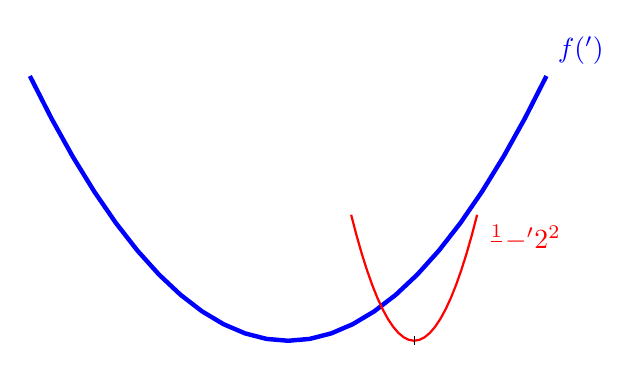
\begin{tikzpicture}[scale=0.8]
					% Original quadratic function
					\draw[blue, ultra thick, domain=-4.1:4.1] plot (\x, {(1/4)*\x*\x}) node[above right] {$f(\weights')$};		
					% Quadratic function with larger curvature, centered at w = 2
					\draw[red, thick, domain=1:3] plot (\x, {2*(\x - 2)*(\x - 2)}) node[below right] {$\frac{1}{\lrate}\normgeneric{\weights-\weights'}{2}^{2}$};
					% Axes
					% Minimum point of second curve
					\draw[shift={(2,0)}] (0pt,2pt) -- (0pt,-2pt) node[below] {$\weights$};
					%\node at (2,0.5) [anchor=north] {$\weights$};
				\end{tikzpicture}
			\end{center}
			\caption{The proximal \gls{operator} updates a \gls{vector} $\weights$ by minimizing a penalized version 
				of the \gls{function} $f(\cdot)$. The \gls{penaltyterm} is the scaled squared \gls{eucliddist} between the optimization 
				variable $\weights'$ and the given \gls{vector} $\weights$.	\label{fig_proxoperator_opt_dict}}
		\end{figure}
		See also: \gls{convex}, \gls{function}, \gls{gradstep}.},
	first={proximal operator},
	type=math,
	firstplural={proximal operators},
	plural={proximal operators},
	text={proximal operator}
}

\newglossaryentry{connected}
{name={connected}, 
	description={An\index{connected} 
		\gls{undirectedgraph} $\graph=\pair{\nodes}{\edges}$ is connected if, for every 
		non-empty subset $\nodes' \subset \nodes$, we can find at least one edge 
		connecting a node in $\nodes'$ with some node in $\nodes \setminus \nodes'$.
		We illustrate two examples of \glspl{undirectedgraph} in Fig. \ref{fig_connected_dict}.
		\begin{figure}[H]
			\centering
			\begin{tikzpicture}
			% Horizontal axis
			% Left graph (single edge)
			\node[circle, fill=black, inner sep=1.5pt, label=above:{1}] (A1) at (0, 1.5) {};
			\node[above=0.5cm of A1, align=center] {disconnected};
			\node[circle, fill=black, inner sep=1.5pt, label=below right:{2}] (B1) [below right=0.8cm and 0.5cm of A1] {};
			\node[circle, fill=black, inner sep=1.5pt, label=below left:{3}] (C1) [below left=0.8cm and 0.5cm of A1] {};
			\draw [line width=1 pt]  (A1) -- (B1);
			\node at (0, -1) {(a)};
			% Middle graph (two edges, shifted right)
			\begin{scope}[xshift=3.5cm]
				\node[circle, fill=black, inner sep=1.5pt, label=above:{1}] (A2) at (0, 1.5) {};
				\node[above=0.5cm of A2, align=center] {connected};
				\node[circle, fill=black, inner sep=1.5pt, label=below right:{2}] (B2) [below right=0.8cm and 0.5cm of A2] {};
				\node[circle, fill=black, inner sep=1.5pt, label=below left:{3}] (C2) [below left=0.8cm and 0.5cm of A2] {};
				\draw [line width=1 pt]  (A2) -- (B2);
				\draw [line width=1 pt]  (B2) -- (C2);
				\node at (0, -1) {(b)};
			\end{scope}
			\end{tikzpicture}
		\caption{(a) A \gls{graph} that is disconnected. (b) A \gls{graph} that is connected. \label{fig_connected_dict}}
		\end{figure} 
		See also: \gls{undirectedgraph}, \gls{algconn}.}, 
	type=math, 
	first={connected},
	text={connected}
}

\newglossaryentry{GaussProc}
{name={Gaussian process (GP)},
	description={A\index{Gaussian process (GP)} GP is a collection of \glspl{rv} 
  		$\{f(\featurevec)\}_{\featurevec \in \featurespace}$ indexed by input values $\featurevec$ 
  		from some input space $\featurespace$ such that, for any finite subset 
  		$\featurevec^{(1)}, \,\ldots, \,\featurevec^{(\samplesize)} \in \featurespace$, 
  		the corresponding \glspl{rv} $f(\featurevec^{(1)}, \,\ldots, \,\featurevec^{(\samplesize)})$ 
		have a joint \gls{mvndist} 
  		\[
  		f \left( \featurevec^{(1)}, \,\ldots, \,\featurevec^{(\samplesize)} \right) \sim \mathcal{N}(\boldsymbol{\mu}, \mathbf{K}).
  		\]
  		For a fixed input space $\featurespace$, a GP is 
		fully specified (or parameterized) by: 1) a \gls{mean} \gls{function} 
		$\mu(\featurevec) = \expect\{ f(\featurevec)\}$; and 2) 
		a \gls{covariance} \gls{function} 
		$\kernelmap{\featurevec}{\featurevec'}= \expect\{ \big(f(\featurevec)-\mu(\featurevec)\big) \big(f(\featurevec')-\mu(\featurevec')\big) \big\}$.\\
  		Example: We can interpret the temperature distribution across Finland (at a specific 
  		point in time) as the \gls{realization} of a GP $f(\featurevec)$, where each input 
		$\featurevec = (\text{lat}, \text{lon})$ denotes a geographic location. Temperature 
		observations from \gls{fmi} weather stations provide values $f(\featurevec)$ at specific 
		locations (see Fig. \ref{fig_gp_FMI_dict}). A GP allows us to predict the temperature 
		nearby \gls{fmi} weather stations and to quantify the \gls{uncertainty} 
  		of these \glspl{prediction}. 
  		\begin{figure}[H]
  		\begin{center}
  			\begin{tikzpicture}
			\begin{axis}[
			axis equal,
			hide axis,
			scale=1.2,
			xmin=17, xmax=32,
			ymin=55, ymax=71,
			%	width=15cm,
			%	height=20cm,
			clip=true
			]
			% --- Finland border (polyline) ---
			\addplot[
			color=black,
			thick
			] table [x=lon, y=lat, col sep=comma] {assets/finland_border.csv};
			% --- FMI sample stations ---
			\addplot[
			only marks,
			mark=*,
			mark options={fill=blue},
			color=black
			] table [x=lon, y=lat, col sep=comma] {assets/fmi_stations_subset.csv};
			% Draw manual axes
			\draw[->, thick] (axis cs:19,59) -- (axis cs:25.5,59) node[anchor=west] {longitude (lon)};
			\draw[->, thick] (axis cs:19,59) -- (axis cs:19,65.5) node[anchor=south] {latitude (lat)};
			\end{axis}
			\end{tikzpicture}
			\vspace*{-5mm}
		\end{center}
		\caption{For a given point in time, we can interpret the current temperature distribution 
		over Finland as a \gls{realization} of a GP indexed by geographic coordinates and 
		sampled at \gls{fmi} weather stations. The weather stations are indicated by blue dots. \label{fig_gp_FMI_dict}}
		\end{figure}
		See also: \gls{mvndist}, \gls{uncertainty}, \gls{gaussrv}.}, 
  	first={GP}, 
  	type=math, 
  	text={GP}
}

\newglossaryentry{normaldist} 
{name={normal distribution}, 
	description={See\index{normal distribution} \gls{gaussrv}, \gls{mvndist}, \gls{clt}.},
 	first={normal distribution}, 
 	firstplural={normal distributions},
 	plural={normal distributions},
	type=math, 
 	text={normal distribution}
}

\newglossaryentry{gaussrv}
{name={Gaussian random variable (Gaussian RV)}, 
	description={A\index{Gaussian random variable (Gaussian RV)} standard \gls{gaussian} \gls{rv} is a 
		real-valued \gls{rv} $\feature$ with \gls{pdf} \cite{BertsekasProb}, \cite{papoulis}, \cite{GrayProbBook}
		\begin{equation}
			\nonumber
			\pdf{\feature}{\eta} = \frac{1}{\sqrt{2\pi}} \exp\,(-\eta^2/2). 
		\end{equation}
		Given a standard \gls{gaussian} \gls{rv} $\feature$, we can construct a general \gls{gaussian} 
		\gls{rv} $\feature'$ with \gls{mean} $\mu$ and \gls{variance} $\sigma^2$ via 
            $\feature' \defeq \sigma \feature + \mu$. 
		The \gls{probdist} of a \gls{gaussian} \gls{rv} is referred to as \gls{normaldist}, 
		denoted by $\mvnormal{\mu}{\sigma^{2}}$. 
		\\ 
		A \gls{gaussian} random \gls{vector} $\featurevec \in \mathbb{R}^{\featuredim}$ with 
		\gls{covmtx} $\mathbf{C}$ and \gls{mean} ${\bm \mu}$ can be constructed as \cite{GrayProbBook}, \cite{papoulis}, \cite{Lapidoth09}
		\[
		\featurevec \defeq \mathbf{A} \vz + {\bm \mu}
		\]
		where $\vz \defeq \big( z_{1}, \,\ldots, \,z_{\featuredim} \big)\,^{T}$ is a \gls{vector} 
		of \gls{iid} standard \gls{gaussian} \glspl{rv}, and $\mA \in \mathbb{R}^{\featuredim \times \featuredim}$ is any \gls{matrix} satisfying $\mA \mA\,^{T} = \mC$. 
		The \gls{probdist} of a \gls{gaussian} random \gls{vector} is referred to as the \gls{mvndist}, 
		denoted by $\mvnormal{\bm \mu}{\mathbf{C}}$.
		\\
		We can interpret a \gls{gaussian} random \gls{vector} $\featurevec=\big(\feature_{1},\,\ldots,\,\feature_{\nrfeatures}\big)^{T}$ as a \gls{stochproc} 
		indexed by the set $\mathcal{I}=\{1,\,\ldots,\,\nrfeatures\}$. A \gls{GaussProc} is a 
		\gls{stochproc} over an arbitray index set $\mathcal{I}$ such that any restriction 
		to a finite subset $\mathcal{I}' \subseteq \mathcal{I}$ yields a \gls{gaussian} 
		random \gls{vector} \cite{Rasmussen2006Gaussian}.
  		\\
        		\Gls{gaussian} \glspl{rv} are widely used \glspl{probmodel} in the 
				statistical analysis of \gls{ml} methods. Their significance arises 
				partly from the \gls{clt} which provides conditions under which 
				the average of many independent \glspl{rv} (not necessarily \gls{gaussian} themselves) 
				tends toward a \gls{gaussian} \gls{rv} \cite{ross2013first}.
		\\ 
		The \gls{mvndist} is also distinct in that it represents \gls{maximum} \gls{uncertainty}. 
		Among all \gls{vector}-valued \glspl{rv} with a given \gls{covmtx} $\mC$, the 
		\gls{rv} $\vx \sim \mvnormal{\bm \mu}{\mathbf{C}}$ maximizes \gls{diffentropy} 
		\cite[Th. 8.6.5]{coverthomas}. This makes \glspl{GaussProc} a natural choice for 
		capturing \gls{uncertainty} or the lack of (domain) knowledge.
		\\ 
		See also: \gls{mvndist}, \gls{GaussProc}, \gls{probmodel}, \gls{clt}, \gls{diffentropy}.},
	first={Gaussian random variable (Gaussian RV)},
	type=math, 
	plural={Gaussian RVs}, 
	firstplural={Gaussian random variables (Gaussian RVs)}, 
	text={Gaussian RV}
}

\newglossaryentry{gaussian} 
{name={Gaussian}, 
	description={See\index{Gaussian} \gls{gaussrv}.},
 	first={Gaussian},
 	type=math,
 	text={Gaussian},
	firstplural={Gaussians},  
 	plural={Gaussians}
}

\newglossaryentry{clt}
{name={central limit theorem (CLT)},
	description={Consider a \gls{sequence} of \gls{iid} \glspl{rv} \( \feature^{(\sampleidx)} \), for \( \sampleidx = 1, \,2, \,\ldots \), 
		each with \gls{mean} zero and finite \gls{variance} \( \sigma^2 > 0 \). 
		The\index{central limit theorem (CLT)} CLT states that the normalized sum 
		\[
		s^{(\samplesize)} \defeq \frac{1}{\sqrt{\samplesize}} \sum_{\sampleidx = 1}^{\samplesize} \feature^{(\sampleidx)} 
		\]
            %%% Should "convergence in distribution" be defined here? Or in a separate entry along with other notions of 
            %%% convergence of random variables? Possibly either way would be ok, it depends how much technical details
            %%% the dictionary is supposed to cover.
		converges in distribution to a \gls{gaussrv} with \gls{mean} zero and \gls{variance} \( \sigma^2 \) as \( \samplesize \to \infty \) \cite[Proposition~2.17]{AsympVanderVaartBook}.
		One elegant way to derive the CLT is via the \gls{characteristicfunc} of the normalized sum \( s^{(\samplesize)} \). 
		Let $ \phi(t) = \expect \big\{ \exp \big( j t \feature \big) \big\}$ (with the imaginary unit $j = \sqrt{-1}$) 
		be the common \gls{characteristicfunc} of each sum and $\feature^{(\sampleidx)}$, and let \( \phi^{(\samplesize)}(t) \) 
		denote the \gls{characteristicfunc} of \( s^{(\samplesize)} \). Define an \gls{operator} \( \mathcal{T} \) acting on \glspl{characteristicfunc} 
		such that
		\[
		\phi^{(\samplesize)}(t) = \mathcal{T}(\phi^{(\samplesize-1)})(t) \defeq \phi\left( \frac{t}{\sqrt{\samplesize}} \right) \cdot \phi^{(\samplesize-1)}\left( \frac{\sqrt{\samplesize-1}}{\sqrt{\samplesize}} t \right).
		\]
		This \gls{fixedpointiter} captures the effect of recursively adding an \gls{iid} \gls{rv} $\featurevec^{(\samplesize)}$ 
		and rescaling. Iteratively applying \( \mathcal{T} \) leads to \gls{convergence} of \( \phi^{(\samplesize)}(t) \) toward the fixed point
		\[
		\phi^*(t) = \exp\,(-t^2 \sigma^2 / 2)
		\]
		which is the \gls{characteristicfunc} of a \gls{gaussrv} with \gls{mean} zero and \gls{variance} 
		\( \sigma^2 \). \Glspl{generalization} of the CLT allow for dependent or nonidentically distributed \glspl{rv} \cite[Sec.~2.8]{AsympVanderVaartBook}.
		\begin{figure}[H]
			\centering
			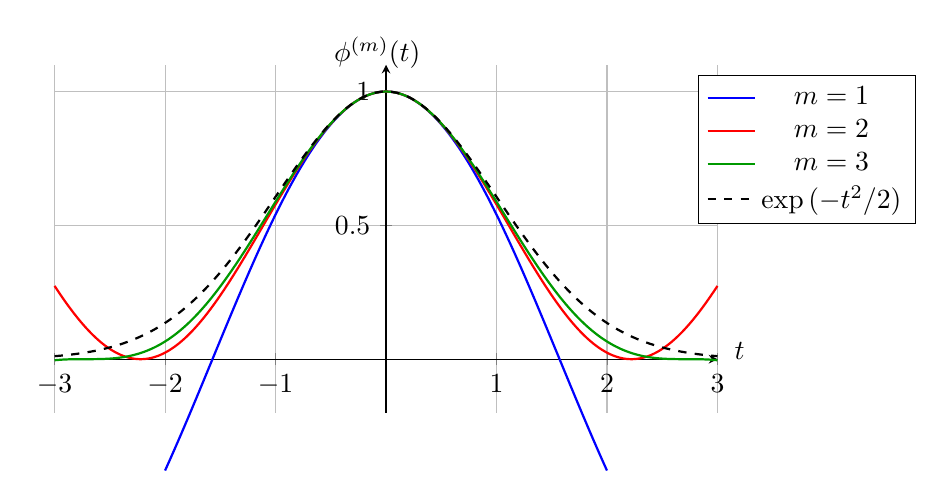
\begin{tikzpicture}
			\begin{axis}[
			width=10cm,
			height=6cm,
			xlabel={},
			ylabel={},
			legend style={at={(0.97,0.97)}, anchor=north west},
			domain=-3:3,
			ylabel style={
			yshift=10pt   % shift label up by 10pt
			},
			samples=400,
			ymin=-0.2, ymax=1.1,
			axis lines=middle,
			clip=false,
			grid=both,
			]
			\addplot[thick, blue,domain=-2:2] {cos(x/sqrt(1) r)^1};
			\addlegendentry{$m=1$}
			\addplot[thick, red] {cos(x/sqrt(2) r)^2};
			\addlegendentry{$m=2$}
			\addplot[thick, green!60!black] {cos(x/sqrt(3) r)^3};
			\addlegendentry{$m=3$}
			\addplot[thick, dashed, black] {exp(-x^2/2)};
			\addlegendentry{$\exp\,(-t^2/2)$}
			\node[anchor=south, rotate=0] at (axis cs:-0.08,1.05) {$\phi^{(m)}(t)$};
			\node[anchor=north, rotate=0] at (axis cs: 3.2,0.1) {$t$};
			\end{axis}
			\end{tikzpicture}
			\caption{\Glspl{characteristicfunc} of normalized sums of \gls{iid} \glspl{rv} $x^{(\sampleidx)} \in \{-1,1\}$ 
			for $\sampleidx=1,\,\ldots,\,\samplesize$ compared to the \gls{gaussian} limit.}
		\end{figure}
		See also: \gls{rv}, \gls{gaussrv}.},
	first={central limit theorem (CLT)},
	type=math, 
	text={CLT}
}

\newglossaryentry{indicatorfunc}
{name={indicator function}, 
  description={Consider some process\index{indicator function} that can result in different possible 
                \glspl{outcome} (e.g., survival or death of a patient). Such 
				a process can be modeled as a \gls{randomexperiment} with 
				\gls{samplespace} $\samplespace$ containing all possible \glspl{outcome}. 
				The \gls{indicatorfunc} $\indicatorfunc{\mathcal{A}}$ of an event 
				$\mathcal{A} \subseteq \samplespace$ is a \gls{function} defined as \cite{BertsekasProb} 
				\[\indicatorfunc{\mathcal{A}}(\outcome) = 
                        \begin{cases}
					1, & \text{if } \outcome \in \mathcal{A}, \\
					0, & \text{if } \outcome \notin \mathcal{A}.
					\end{cases}
				\]
				The notion of an indicator \gls{function} is not limited to \glspl{outcome} of 
				a \gls{randomexperiment}. Ultimately, it is just a principled way to 
				represent a set $\mathcal{A}$ by a \gls{function} $\indicatorfunc{\mathcal{A}}$ \cite{BoydConvexBook}.
                    For a \gls{probspace} $(\samplespace, \sigmaalgebra, \prob{\cdot})$ and $\mathcal{A} \in \sigmaalgebra$, the indicator \gls{function} $\indicatorfunc{\mathcal{A}}$ is a \gls{rv} and it holds that $\expect\{\indicatorfunc{\mathcal{A}}\} = \prob{\mathcal{A}}$.}, 
  first={indicator function},
  plural={indicator functions}, 
  type=math, 
  text={indicator function}
}

\newglossaryentry{probmodel}
{name={probabilistic model}, 
	description={A probabilistic \gls{model}\index{probabilistic model} for the 
				  generation of \glspl{datapoint} consists of \glspl{rv} 
				  with a joint \gls{probdist} \cite{BertsekasProb}. 
				  This joint \gls{probdist} typically involves \glspl{parameter} (or \glspl{modelparam}) 
				  that are either chosen manually or learned via statistical inference 
				  methods such as \gls{maxlikelihood} estimation \cite{LC}.
					\\ 
		See also: \gls{model}, \gls{datapoint}, \gls{rv}, \gls{probdist}, \gls{parameter}, \gls{maxlikelihood}, \gls{realization}. }, 
	first={probabilistic model}, 
	plural={probabilistic models},
	firstplural={probabilistic models},
	type=math,
	text={probabilistic model} 
}

\newglossaryentry{mean}
{name={mean}, plural={means},
	description={The\index{mean} mean of an \gls{rv} $\featurevec$, which takes 
 		on values in a \gls{euclidspace} $\mathbb{R}^{\dimlocalmodel}$, is its 
 		\gls{expectation} $\expect\{\featurevec\}$. It is defined as the Lebesgue 
 		integral of $\featurevec$ with respect to the underlying \gls{probdist} $\prob{}$ (e.g., 
		see \cite{RudinBookPrinciplesMatheAnalysis} or \cite{BillingsleyProbMeasure}), i.e.,
		\[
                \expect\{\featurevec\} = \int_{\mathbb{R}^{\dimlocalmodel}} \vx \, \mathrm{d}P(\vx).
		\]  
            %%% are we assuming a density function here to keep the presentation simple? 
            %%% otherwise, P(\vx) is to be interpreted as a "push-forward measure" from the probability space to $\mathbb{R}^{\dimlocalmodel}$?
		We also use the term to refer to the \gls{samplemean} of a finite \gls{dataset}
		$\dataset = \left\{ \vx^{(1)}, \,\ldots, \,\vx^{(\samplesize)} \in \mathbb{R}^{\dimlocalmodel}\right\}$. 
		However, these two definitions are essentially the same. Indeed, we can use 
		a \gls{dataset} to construct a discrete \gls{rv} $\widetilde{\vx}^{(\dataset)}=\vx^{(I)}$ on 
		the \gls{samplespace} $\{1, \,\ldots, \,\samplesize\}$. Here, the index $I$ is 
		chosen uniformly at random, $\prob{I=\sampleidx}=1/\samplesize$ for all 
		$\sampleidx=1,\ldots,\samplesize$. The mean of $\widetilde{\vx}^{(\dataset)}$ is 
		precisely the average $({1}/{\samplesize}) \sum_{\sampleidx=1}^{\samplesize} \vx^{(\sampleidx)}$.
		For an \gls{rv} with finite second-order moment, i.e., 
		$\expect\{ \normgeneric{\featurevec}{2}^{2} \}$ is well-defined and fnite, 
		the mean is characterized as the solution of the 
		following \gls{risk} minimization problem \cite{BertsekasProb}:
		\[
			\expect\{\featurevec\} = \argmin_{\vc \in \mathbb{R}^{\nrfeatures}} 
			\expect \big\{\normgeneric{\featurevec - \vc}{2}^{2}\big \}.
		\]
		For the \gls{rv} $\widetilde{\vx}^{(\dataset)}$, associated with a \gls{dataset} $\dataset$, 
		this \gls{optproblem} reduces to \gls{erm} with \gls{sqerrloss} on $\dataset$. 
		\\ 
		See also: \gls{rv}, \gls{expectation}, \gls{probdist}, \gls{erm}.}, 
	first={mean}, 
	type=math,
	text={mean} 
}

\newglossaryentry{median}
{name={median}, 
plural={medians},
	description={A\index{median} median $\med\,(x)$ of a real-valued \gls{rv} $x$ 
 		is any number $M \in \mathbb{R}$ such that $\prob{ x \leq M} \geq 1/2$ and 
		$\prob{ x \geq M} \geq 1/2$ 
		(see Fig. \ref{fig_median1_dict}) \cite{LC}. 
 		\begin{figure}[H]
			\begin{center}
			\begin{tikzpicture}
 			\begin{axis}[
    			axis lines=middle,
    			xlabel={},
    			ylabel={},
    			ymin=0, ymax=1.1,
    			xmin=-2, xmax=6,
    			xtick=\empty,
    			ytick={0,1/2,1},
    			domain=-2:6,
    			samples=200,
    			width=10cm,
    			height=6cm,
    			smooth,
    			enlargelimits=true,
    			clip=false
  			]
    			% Shifted sigmoid CDF
			\addplot[thick, blue, name path=cdf] {1/(1 + exp(-(x - 1)))} node[pos=0.5, above, yshift=15pt] {$\prob{x \leq \eta}$};    % Vertical and horizontal ruler at F(x) = 0.5
    			\draw[dashed, gray] (axis cs:1,0) -- (axis cs:1,0.5); % vertical
    			\draw[dashed, gray] (axis cs:-2,0.5) -- (axis cs:1,0.5); % horizontal
    			% Mark the median point
   			\filldraw[red] (axis cs:1,0.5) circle (2pt);
  		    	\node[below] at (axis cs:1,0) {$M$};
			\node[above right] at (axis cs:6.3,0) {$\eta$};
    			% Label next to curve
  			\end{axis}
			\end{tikzpicture} 
			\end{center}
		\caption{The median of a real-valued \gls{rv} is any number $M$ 
			that partitions $\mathbb{R}$ into two rays with equal \gls{probability}. \label{fig_median1_dict}}
 		\end{figure}  
 		We can define the median $\med\,(\dataset)$ 
 		of a \gls{dataset} $\dataset = \{ x^{(1)}, \,\ldots, \,x^{(\samplesize)} \in \mathbb{R} \}$ 
 		via a specific \gls{rv} $\tilde{x}^{(\dataset)}$ that is naturally associated with $\dataset$. 
 		In particular, this \gls{rv} is defined on the \gls{samplespace} $\{1, \,\ldots, \,\samplesize\}$ 
		via $\tilde{x}^{(\dataset)} \defeq x^{(I)}$. Here, the index $I$ is chosen uniformly 
		at random, i.e., $\prob{I = \sampleidx}=1/\samplesize$ for 
 		all $\sampleidx=1, \,\ldots, \,\samplesize$. If the \gls{rv} $x$ is integrable, any 
		median of $x$ solves the \gls{optproblem}: 
 		$$\min_{x' \in \mathbb{R}} \expect{|x - x'|}.$$ 
		For a the above \gls{rv} $\tilde{x}$ (constructed from a \gls{dataset} $\dataset$), 
		this \gls{optproblem} is \gls{erm} on $\dataset$ using \gls{abserr}. 
 		Like the \gls{mean}, the median of a \gls{dataset} $\dataset$ can also be used 
 		to estimate \glspl{parameter} of an underlying \gls{probmodel}. Compared 
 		with the \gls{mean}, the median is more robust to \glspl{outlier}. For example, 
 		a median of a \gls{dataset} $\dataset$ with more than one \gls{datapoint} does not 
 		change even if we arbitrarily increase the largest element of $\dataset$ (see Fig. \ref{fig_median2_dict}). 
		In contrast, the \gls{mean} will increase arbitrarily.
		\begin{figure}[H]
		\centering
		\begin{tikzpicture}[scale=0.7, y=0.5cm, x=0.5cm]
			\begin{scope}
				\foreach \x/\y in {
					1/2, 4/3, 7/4
				} {
					\draw[dashed, gray] (\x, 0) -- (\x, \y);
					\filldraw[blue] (\x, \y) circle (2pt);
					\node[circle, inner sep=0pt] (ptA\x) at (\x, \y) {};
				}
				\draw[dashed, thick] (0.5, 3) -- (10.5, 3) node[right] {$\med\,(\dataset)\!=\!{\rm mean}(\dataset)$};
				\node at (7.5, -4) {(a)};
			\end{scope}
			\begin{scope}[xshift=12cm]
				\foreach \x/\y in {
					1/2, 4/3, 7/10
				} {
					\draw[dashed, gray] (\x, 0) -- (\x, \y);
					\filldraw[blue] (\x, \y) circle (2pt);
					\node[circle, inner sep=0pt] (ptB\x) at (\x, \y) {};
				}
				\draw[dashed, thick] (0.5, 7.5) -- (10.5, 7.5) node[right] 
				{${\rm mean}\,\big(\widetilde{\dataset}\big)$};
				\draw[dashed, thick] (0.5, 3) -- (10.5, 3) node[right] 
				{$\med\,\big(\widetilde{\dataset}\big)$};
				\node[above right=2pt and 2pt, red] at (ptB7) {\gls{outlier}};
				\node at (7.5, -4) {(b)};
			\end{scope}
		\end{tikzpicture}
		\caption{The median is robust against \gls{outlier} contamination. (a) Original \gls{dataset} $\dataset$. (b) Noisy 
			\gls{dataset} $\widetilde{\dataset}$ including an \gls{outlier}. \label{fig_median2_dict}}
		\end{figure}
		See also: \gls{mean}, \gls{outlier}, \gls{robustness}, \gls{ladregression}.}, 
	first={median}, 
	type=math,
	text={median} 
}

\newglossaryentry{variance}
{name={variance},
	description={The\index{variance} variance of a real-valued \gls{rv} $\feature$ is defined 
	   	as the \gls{expectation} $\expect\big\{ \big( x - \expect\{x \} \big)^{2} \big\}$ of 
	   	the squared difference between $\feature$ and its \gls{expectation} $\expect\{x \}$. 
	   	We extend this definition to \gls{vector}-valued \glspl{rv} $\featurevec$ 
	   	as $\expect\big\{ \big\| \featurevec - \expect\{\featurevec \} \big\|_{2}^{2} \big\} = \tr{\covmtx{\featurevec}}$,
          	i.e., the sum of the variances of each entry of $\featurevec$, which can be written compactly 
		as the \gls{trace} of the \gls{covmtx} $\covmtx{\featurevec}$ of $\featurevec$. 
          	\\ 	 
		See also: \gls{rv}, \gls{expectation}, \gls{vector}.},
	first={variance},
	type=math,
	text={variance} 
}

\newglossaryentry{probabilitysimplex}
{name={probability simplex},
	description={The\index{probability simplex} \gls{probability} simplex
   		$\simplex{\nrcluster-1}$ is the set of all \glspl{vector} 
   		in $\mathbb{R}^\nrcluster$ with nonnegative entries 
 		that sum to one \cite{BoydConvexBook}. Each element of $\simplex{\nrcluster-1}$ 
		represents a \gls{pmf} of an \gls{rv} $y \in \{1,\,\ldots,\,\nrcluster\}$.
		\\
		See also: \gls{probability}, \gls{vector}, \gls{pmf}, \gls{rv}. },
  	first={probability simplex},
  	plural={probability simplexes},
  	firstplural={probability simplexes},
  	type=math,
  	text={probability simplex}
}

\newglossaryentry{projection}
{name={projection}, 
       	description={Consider\index{projection} a bounded subset 
		$\paramspace \subseteq \mathbb{R}^{\dimlocalmodel}$ of 
		the $\dimlocalmodel$-dimensional \gls{euclidspace}. We define the projection 
		$\projection{\paramspace}{\weights}$ of a \gls{vector} 
		$\weights \in \mathbb{R}^{\dimlocalmodel}$ onto $\paramspace$ as
	   	\begin{equation} 
   	   		\nonumber
			\label{equ_def_proj_generic_dict}
  	    		\projection{\paramspace}{\weights} = \argmin_{\weights' \in \paramspace} \normgeneric{\weights - \weights'}{2}. 
        	    	\end{equation}
	    	In other words, $\projection{\paramspace}{\weights}$ is the \gls{vector} in $\paramspace$ 
	    	that is closest to $\weights$. The projection is only well defined for subsets $\paramspace$ 
	    	for which the above \gls{minimum} exists \cite{BoydConvexBook}.
		 			\\ 
	    	See also: \gls{euclidspace}, \gls{vector}, \gls{minimum}.},
	first={projection},
	type=math,
	text={projection}
}

\newglossaryentry{projgd}
{name={projected gradient descent (projected GD)},
	description={Consider an \gls{erm}-based method that uses a parameterized \gls{model} with  
		\gls{paramspace} $\paramspace \subseteq \mathbb{R}^{\dimlocalmodel}$. Even if 
		the \gls{objfunc} of \gls{erm} is \gls{smooth}, we cannot use basic \gls{gd}, as 
		it does not take into account constraints on the optimization variable (i.e., the \glspl{modelparam}). 
		Projected\index{projected gradient descent (projected GD)} \gls{gd} 
		extends basic \gls{gd} to address this issue. 
		A single iteration of projected \gls{gd} consists of first taking a \gls{gradstep} 
		and then projecting the result back onto the \gls{paramspace}. 
		See Fig. \ref{fig_projected_GD_dict} for a visual illustration.
		\begin{figure}[H]
		\begin{center}
			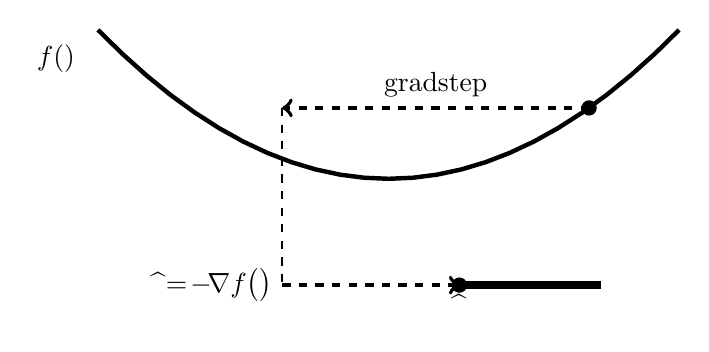
\begin{tikzpicture}[scale=0.9]
			\node [right] at (-5.1,1.7) {$f(\weights)$} ;
			\draw[ultra thick, domain=-4.1:4.1] plot (\x,  {(1/8)*\x*\x});
		%	\draw[dashed, thick, domain=1:3.6] plot (\x,  {\x - 1}) node[right] {$ f\big(\weights^{(\itercntr)}\big)\!+\!\big(\weights\!-\!\weights^{(\itercntr)}\big)^{T} \nabla f\big(\weights^{(\itercntr)}\big)$};
			\draw [fill] (2.83,1) circle [radius=0.1] node[right] {$\weights$};
			\draw[line width =0.5mm,dashed,->] (2.83,1) -- node[midway,above] {\gls{gradstep}} (-1.5,1);
			\draw[line width =0.2mm,dashed] (-1.5,1) --(-1.5,-1.5)  node [below, left]{$\widehat{\weights}=\weights\!-\!\lrate \nabla f\big(\weights\big)$} ;
			\draw[line width =0.5mm,dashed,->] (-1.5,-1.5)  -- node[midway,above] {} (1,-1.5) ; 
			\draw [fill] (1,-1.5) circle [radius=0.1] node[below] {$\projection{\paramspace}{\widehat{\weights}}$};
			\draw[line width=1mm] (1,-1.5) -- (3,-1.5) node[midway, above] {$\paramspace$};
			\end{tikzpicture}
		\vspace*{-5mm}
		\end{center}
		\caption{Projected \gls{gd} augments a basic \gls{gradstep} with a \gls{projection} back 
			onto the constraint set $\paramspace$.}
			\label{fig_projected_GD_dict}
		\end{figure}
		See also: \gls{erm}, \gls{model}, \gls{paramspace}, \gls{objfunc}, \gls{smooth}, \gls{gd}, \gls{modelparam}, \gls{gradstep}, \gls{projection}.},
	first={projected gradient descent (projected GD)},
	type=math, 
	text={projected GD}
}

\newglossaryentry{proximable}
{name={proximable},
	description={A\index{proximable} 
		\gls{convex} \gls{function} for which the \gls{proxop} can be computed efficiently is 
		sometimes referred to as proximable or simple \cite{Condat2013}.
					\\ 
		See also: \gls{convex}, \gls{function}, \gls{proxop}.},
	first={proximable},
	type=math,
	text={proximable}
}

\newglossaryentry{operator} 
{name={operator}, 
	description={An\index{operator} operator is a \gls{function} 
		whose \gls{domain} and \gls{co-domain} have a specific 
		mathematical structure such as a \gls{vectorspace}, a \gls{hilbertspace},
		or a \gls{metricspace} \cite{Bauschke:2017}, \cite{DunfordSchwartz1988}. 
		Many \gls{ml} methods involve operators whose \gls{domain} and \gls{co-domain} 
		are \glspl{euclidspace}.
							\\ 
		See also: \gls{function}, \gls{vectorspace}, \gls{hilbertspace}.},
	first={operator},
	type=math, 
	plural={operators},
	firstplural={operators},
	text={operator}
}

\newglossaryentry{ergraph}
{name={Erd\H{o}s–R\'enyi graph (ER graph)},
	description={An ER \gls{graph}\index{Erd\H{o}s–R\'enyi graph (ER graph)} \cite{erdds1959random}, \cite{gilbert1959random} 
            	is a \gls{probmodel} for \glspl{graph} defined over a given node set $\nodeidx=1, \,\ldots, \,\nrnodes$. 
            	One way to define the ER \gls{graph} is via the collection of \gls{iid} binary 
            	\glspl{rv} $b^{(\edge{\nodeidx}{\nodeidx'})} \in \{0,1\}$, 
		for each pair of different nodes $\nodeidx, \nodeidx'$. A specific \gls{realization}  
		of an ER \gls{graph} contains an edge $\edge{\nodeidx}{\nodeidx'}$ if and only if 
		$b^{(\edge{\nodeidx}{\nodeidx'})}=1$. The ER \gls{graph} is parameterized by the 
		number $\nrnodes$ of nodes and the \gls{probability} $\prob{b^{(\edge{\nodeidx}{\nodeidx'})}=1}$.	
		\\
		See also: \gls{graph}, \gls{probmodel}, \gls{iid}, \gls{rv}, \gls{realization}, \gls{probability}.},
	first={Erd\H{o}s–R\'enyi graph (ER graph)},
	type=math,
	text={ER graph}
}

\newglossaryentry{condprobdist}
{name={conditional probability distribution}, 
	description={Consider\index{conditional probability distribution} 
     		a \gls{stochproc} consisting of two \glspl{rv} $\featurevec$ and $\truelabel$ 
    		with \gls{probdist} $\probdist^{(\featurevec,\truelabel)}$. The conditional 
    		\gls{probdist} of $\truelabel$ given (or conditioned on) $\featurevec$ is 
    		denoted by $\probdist^{(\truelabel\mid\featurevec)}$. It is defined via the 
    		\glspl{conditionalexpect} of the \glspl{indicatorfunc} of  
    		\gls{measurable} sets in the \gls{sigmaalgebra} generated by 
    		the \gls{rv} $\truelabel$ \cite{BillingsleyProbMeasure}, \cite{KallenbergBook}.
		\\
		See also: \gls{probdist}, \gls{conditionalexpect}. },
  	first={conditional probability distribution}, 
  	plural={conditional probability distributions},
  	type=math, 
  	text={conditional probability distribution}
}

\newglossaryentry{linearmap}
{name={linear map}, plural={linear maps}, 
	description={A\index{linear map} linear \gls{map} 
		$f: \mathbb{R}^\nrfeatures \rightarrow \mathbb{R}^\samplesize$ 
	    	is a \gls{function} that satisfies additivity, i.e.,
		$f(\vx + \vy) = f(\vx) + f(\vy)$, and homogeneity, i.e.,
		$f(c\vx) = c f(\vx)$, for all \glspl{vector} $\vx, \vy \in \mathbb{R}^\nrfeatures$ 
		and scalars $c \in \mathbb{R}$. In particular, $f(\mathbf{0}) = \mathbf{0}$. 
		Any linear \gls{map} can be represented as a \gls{matrix} multiplication 
		$f(\vx) = \mA \vx$, for some \gls{matrix} $\mA \in \mathbb{R}^{m \times n}$. 
		The collection of real-valued linear \glspl{map} (where $\samplesize=1$), 
		for a given dimension $\nrfeatures$, constitute a \gls{linmodel}. The notion 
		of a linear \gls{map} can be generalized from the \gls{domain} $\mathbb{R}^{\nrfeatures}$ 
		and \gls{co-domain} $\mathbb{R}^{\samplesize}$ to arbitrary \glspl{vectorspace}.
		\\
		See also: \gls{map}, \gls{function}, \gls{vector}, \gls{matrix}, \gls{linmodel}.},
	first={linear map},
	type=math, 
	plural={linear maps}, 
	firstplural={linear maps}, 
	text={linear map}
}

\newglossaryentry{vector}
{name={vector},
	description={A\index{vector} vector is an element of a \gls{vectorspace}. 
		In the context of \gls{ml}, a particularly important example of a \gls{vectorspace} 
		is the \gls{euclidspace} $\mathbb{R}^{\nrfeatures}$, where $\nrfeatures \in \mathbb{N}$ 
		is the (finite) dimension of the space. A vector $\vx \in \mathbb{R}^{\nrfeatures}$ 
		can be represented as a list or one-dimensional (1-D) array of real numbers, i.e., 
		$x_1, \,\ldots, \,x_{\nrfeatures}$ with $x_\featureidx \in \mathbb{R}$ for 
		$\featureidx = 1, \,\ldots, \,\nrfeatures$. The value $x_\featureidx$ is the $\featureidx$th 
		entry of the vector $\vx$. It can also be useful to view a vector $\vx \in \mathbb{R}^{\nrfeatures}$ 
		as a \gls{function} that maps each index $\featureidx \in \{1, \,\ldots, \,\nrfeatures\}$ 
		to a value $x_\featureidx \in \mathbb{R}$, i.e., $\vx: \featureidx \mapsto x_\featureidx$. 
		This perspective is particularly useful for the study of \glspl{kernelmethod}. See Fig. 
		\ref{fig:vector-function-dual_dict} for the two views of a vector.
		\begin{figure}[H]
			% Left: Stem plot
			\begin{minipage}[c]{0.48\textwidth}
				\centering 
				2, --1, 3, 0, --2, 1
				\begin{minipage}{\textwidth}
				\vspace{5ex}
				\centering
				{\selectfont (a)}
				\end{minipage}
			\end{minipage}
			\hfill
			% Right: Column vector
			\begin{minipage}{0.48\textwidth}
			\centering
			\begin{tikzpicture}
			\begin{axis}[
    				width=6.5cm,
    				height=5cm,
    				title={},
    				xlabel={index $\featureidx$},
    				ylabel={$x_\featureidx$},
   		 		ymin=-3.5, ymax=3.5,
    				xmin=0.5, xmax=6.5,
   	 			xtick={1,2,3,4,5,6},
    				ytick={-3,-2,-1,0,1,2,3},
    				axis x line=bottom,        % <-- horizontal axis at y=0
    				axis y line=left,          % <-- vertical axis on the left
    				grid=both,
    				major grid style={dotted, gray!60},
    				enlargelimits=0.1
			]
			\addplot+[ycomb, thick, mark=*]
    			coordinates {
        				(1,2)
        				(2,-1)
       	 			(3,3)
        				(4,0)
        				(5,-2)
        				(6,1)
    			};
			\end{axis}
			\node at (2,-2.5) {(b)};
			\end{tikzpicture}
			\end{minipage}
		\caption{Two equivalent views of a vector $\vx= \big( 2, -1, 3, 0, -2, 1 \big)^{T} \in \mathbb{R}^{6}$.
			(a) As a numeric array. (b) As a \gls{map} $\featureidx \mapsto x_\featureidx$.}
			\label{fig:vector-function-dual_dict}
		\end{figure}
		See also: \gls{vectorspace}, \gls{euclidspace}, \gls{linearmap}.},
	first={vector},
	firstplural={vectors},
	type=math,
	plural={vectors},
	text={vector}
}

\newglossaryentry{vectorspace}
{name={vector space},
	description={A\index{vector space} \gls{vector} space $\mathcal{V}$ (also called linear space) 
		is a collection of elements, called \glspl{vector}, along with the following two operations 
		(see also Fig. \ref{fig:vector-ops_dict}): 
    		1) addition (denoted by $\vv+\vw$) of two \glspl{vector} $\vv,\vw$; and 2) multiplication 
		(denoted by $c \,\cdot \,\vv$) of a \gls{vector} $\vv$ with a scalar $c$ that belongs to some 
		number field (such as the real numbers $\mathbb{R}$ or the complex numbers $\mathbb{C}$). The defining 
		property of a \gls{vector} space is that it is closed under two specific operations. First, 
		if $\vv, \vw \in \mathcal{V}$, then $\vv + \vw \in \mathcal{V}$. Second, if $\vv \in \mathcal{V}$ 
		and $c \in \mathbb{R}$, then $c \vv \in \mathcal{V}$.
		\begin{figure}[H]
		\centering
			\begin{tikzpicture}[>=Stealth, scale=1.2]
			% Coordinates
  			\coordinate (O) at (0,0);            % Origin
  			\coordinate (V) at (2,1.5);          % vector v
  			\coordinate (W) at (1,3);            % vector w
  			\coordinate (VplusW) at (3,4.5);     % v + w
  			\coordinate (HalfV) at (1,0.75);     % 0.5 * v
  			\draw[->, thick, blue] (O) -- (V) node[pos=1, right] {$\vv$};
  			\draw[->, thick, red] (O) -- (W) node[pos=1, left] {$\vw$};
  			\draw[->, thick, purple] (O) -- (VplusW) node[pos=0.99, above right] {$\vv+\vw$};
  			\draw[dashed, red] (V) -- (VplusW);
  			\draw[dashed, blue] (W) -- (VplusW);
  			\draw[->, thick, orange] (O) -- (HalfV) node[midway, right] {$ \alpha \vv$};
			% Filled dots
  			\filldraw[black] (O) circle (2pt) node[below left] {$\mathbf{0}$};  % origin
  			\filldraw[blue] (V) circle (2pt);         % v
  			\filldraw[red] (W) circle (2pt);          % w
  			\filldraw[purple] (VplusW) circle (2pt);  % v + w
  			\filldraw[orange] (HalfV) circle (2pt);   % 0.5v
			\end{tikzpicture}
			\caption{A \gls{vector} space $\mathcal{V}$ is a collection of \glspl{vector} such that 
			scaling and adding them always yields another \gls{vector} in $\mathcal{V}$.}
			%In \gls{ml}, we use vector spaces to represent \glspl{rv}, \glspl{datapoint} 
			%(or their \glspl{featurevec}) as well as invariances (or symmetries) of \glspl{model}.}
			\label{fig:vector-ops_dict}
		\end{figure}
		A common example of a \gls{vector} space is the \gls{euclidspace} $\mathbb{R}^n$, which is 
		widely used in \gls{ml} to represent \glspl{dataset}. We can also use $\mathbb{R}^n$ 
		to represent, either exactly or approximately, the \gls{hypospace} used by an \gls{ml} method.  
		Another example of a \gls{vector} space, which is naturally associated with every \gls{probspace} 
		$\big(\samplespace,\eventspace,\prob{\cdot} \big)$, is the collection of all 
		real-valued \glspl{rv} $x: \samplespace \rightarrow \mathbb{R}$ \cite{RudinBook}, \cite{folland1999real}.  
		\\
		See also: \gls{vector}, \gls{euclidspace}, \gls{linmodel}, \gls{linearmap}.},
	first={vector space},
	plural={vector spaces}, 
	firstplural={vector spaces}, 
	type=math,
	text={vector space}
}

\newglossaryentry{stochastic}
{name={stochastic},
	description={We refer to a\index{stochastic} method as stochastic if it involves a 
		random component or is governed by probabilistic laws. \Gls{ml} methods use randomness 
		to reduce computational complexity (e.g., see \gls{stochGD}) or 
		to capture \gls{uncertainty} in \glspl{probmodel}.
		\\
		See also: \gls{stochGD}, \gls{uncertainty}, \gls{probmodel}.},
	first={stochastic},
	type=math, 
	text={stochastic}
}

\newglossaryentry{stochproc}
{name={stochastic process},
	description={A \gls{stochastic} process\index{stochastic process} is a collection of 
		\glspl{rv} defined on a common \gls{probspace} and indexed by some set 
		$\mathcal{I}$ \cite{GrayProbBook}, \cite{papoulis}, \cite{Brockwell91}. The index set 
		$\mathcal{I}$ typically represents time or space, allowing us to represent 
		random phenomena that evolve across time or spatial dimensions—for example, 
		sensor noise or financial time series. \Gls{stochastic} processes are not limited 
		to temporal or spatial settings. For instance, random \glspl{graph} such as 
		the \gls{ergraph} or the \gls{sbm} can also be viewed as \gls{stochastic} processes. 
		Here, the index set $\mathcal{I}$ consists of node pairs that index \glspl{rv} whose values 
		encode the presence or weight of an edge between two nodes. Moreover, \gls{stochastic} 
		processes naturally arise in the analysis of \glspl{stochalgorithm}, 
		such as \gls{stochGD}, which construct a \gls{sequence} of \glspl{rv}. 
		\\
		See also:  \gls{rv}, \gls{sbm}, \gls{stochGD}, \gls{uncertainty}, \gls{probmodel}.},
	first={stochastic process},
	firstplural={stochastic processes},
	type=math, 
	plural={stochastic processes},
	text={stochastic process}
}

\newglossaryentry{characteristicfunc}
{name={characteristic function},
	description={The characteristic \gls{function}\index{characteristic function} 
		of a real-valued \gls{rv} $x$ is the \gls{function} \cite[Sec. 26]{BillingsleyProbMeasure}
		$$ \phi_{x}(t) \defeq \expect { \exp\,(j t x) } \mbox{ with } j = \sqrt{-1}.$$
	 	The characteristic \gls{function} uniquely determines the \gls{probdist} of $x$. 
		\\
		See also: \gls{rv}, \gls{probdist}.},
	first={characteristic function},
	firstplural={characteristic functions}, 
	type=math, 
	plural={characteristic functions},
	text={characteristic function}
}

\newglossaryentry{entropy}
{name={entropy},
	description={Entropy\index{entropy} quantifies the \gls{uncertainty} or 
		unpredictability associated with an \gls{rv} \cite{coverthomas}. 
		For a \gls{discreteRV} $x$ taking on values in a finite set 
		$\mathcal{S} = \{x_1, \,\ldots, \,x_\nrcluster\}$ with 
		a \gls{pmf} $\pmf{x}{x_{\clusteridx}} (=\prob{x = x_{\clusteridx}})$, 
		the entropy is defined as \cite{coverthomas}
		\[
		   \entropy{x} \defeq -\sum_{\clusteridx=1}^{\nrcluster} \pmf{x}{x_{\clusteridx}}  \log \pmf{x}{x_{\clusteridx}} .
		\]
		For a given set of values $\mathcal{S}$, the entropy is maximized for a 
		uniformly distributed \gls{rv}, where $\pmf{x}{x_{\clusteridx}}=1/\nrcluster$. 
		The minimal entropy, which is zero, is obtained when $\pmf{x}{x_{\clusteridx}}=1$ 
		for some $x_{\clusteridx} \in \mathcal{S}$.
		\Gls{diffentropy} generalizes the concept of \gls{entropy} from \glspl{discreteRV} to 
		\gls{continuous} \glspl{rv}. 
		\\
		See also: \gls{uncertainty}, \gls{probmodel}.},
	first={entropy},
	type=math, 
	text={entropy}
}

\newglossaryentry{diffentropy}
{name={differential entropy},
	description={For\index{differential entropy} an 
		\gls{rv} $\featurevec \in \mathbb{R}^{\nrfeatures}$ 
		with a \gls{pdf} $\pdf{x}{\cdot}$, the differential \gls{entropy} 
		is defined as \cite{coverthomas}
		\[
		h(\featurevec) \defeq - \int_{\featurevec' \in \mathbb{R}^{\nrfeatures}} 
            %\log p(\featurevec') \, d \pdf{\featurevec}{\featurevec'} .
		\log p(\featurevec') \pdf{\featurevec}{\featurevec'} \, d \featurevec'.
            \]
		Differential \gls{entropy} can be negative and lacks some properties of 
		\gls{entropy} for discrete-valued \glspl{rv}, such as invariance under 
		a change of variables \cite{coverthomas}. Among all \glspl{rv} with a 
		given \gls{mean} $\meanvecgeneric$ and \gls{covmtx} $\covmtxgeneric$, 
		$h(\featurevec)$ is maximized by $\featurevec \sim \mvnormal{\meanvecgeneric}{\covmtxgeneric}$. 
		\\
		See also: \gls{uncertainty}, \gls{probmodel}.},
	first={differential entropy},
	type=math,
	text={differential entropy}
}

\newglossaryentry{domain}
{name={domain}, 
	description={The domain\index{domain} of a \gls{function} 
		$f: \mathcal{U} \rightarrow \mathcal{V}$ is the set $\mathcal{U}$ 
		from which $f$ takes its inputs.  
		\\
		See also: \gls{function}, \gls{co-domain}, \gls{map}.},
	first={domain},
	firstplural={domains}, 
	type=math, 
	plural={domains},
	text={domain}
}

\newglossaryentry{function}
{name={function}, 
	description={A function\index{function} between two sets $\mathcal{U}$ and $\mathcal{V}$ assigns  
		each element $u \in \mathcal{U}$ exactly one element $f(u) \in \mathcal{V}$ \cite{RudinBookPrinciplesMatheAnalysis}.
		We write this as $$f: \mathcal{U} \rightarrow \mathcal{V}: u \mapsto f(u)$$ 
		where $\mathcal{U}$ is the \gls{domain} and $\mathcal{V}$ the \gls{co-domain} of $f$. 
		That is, a function $f$ defines a unique \gls{output} $f(u) \in \mathcal{V}$ for every 
		input $u \in \mathcal{U}$ (see Fig. \ref{fig_function_dict}).
		\begin{figure}[H]
			\centering
			\begin{tikzpicture}[>=stealth, node distance=1.2cm and 2.5cm]
				\tikzset{dot/.style={circle, fill=black, inner sep=1.2pt}}
				\node (A) [dot, label=left:$a$] {};
				\node (B) [dot, below=of A, label=left:$b$] {};
				\node (C) [dot, below=of B, label=left:$c$] {};
				\node (1) [dot, right=4cm of A, label=right:$\star$] {};
				\node (2) [dot, below=of 1, label=right:$\circ$] {};
				\node (3) [dot, below=of 2, label=right:$\otimes$] {};
				\node[draw=blue!70, thick, ellipse, inner sep=0.5cm, fit=(A)(B)(C), label=above:$\mathcal{U}$] {};
				\node[draw=green!70!black, thick, ellipse, inner sep=0.5cm, fit=(1)(2)(3), label=above:$\mathcal{V}$] {};
				\draw[->] (A) -- (2);
				\draw[->] (B) -- (1);
				\draw[->] (C) -- (2);
			\end{tikzpicture}
			\caption{A function \( f \colon \mathcal{U} \to \mathcal{V} \) mapping each element 
				of the \gls{domain} $\mathcal{U} =  \{a,b,c\}$ to exactly one element of 
				the \gls{co-domain} $\mathcal{V} = \{\star,\circ,\otimes\}$. \label{fig_function_dict}}
		\end{figure} 
		See also: \gls{domain}, \gls{co-domain}, \gls{output}. },
	first={function},
	firstplural={functions}, 
	type=math, 
	plural={functions},
	text={function}
}

\newglossaryentry{map}
{name={map}, 
	description={We\index{map} use the term map as a synonym for \gls{function}.
		\\
		See also: \gls{function}.},
	first={map},
	firstplural={maps},	
	type=math, 
	plural={maps},
	text={map}
}

\newglossaryentry{event}
{name={event}, 
	description={Consider\index{event} an \gls{rv} $\featurevec$, defined on some \gls{probspace}, 
		which takes values in a \gls{measurable} space $\featurespace$. An 
		event $\mathcal{A} \subseteq \featurespace$ is a subset of $\featurespace$ 
		such that the \gls{probability} $\prob{\featurevec \in \mathcal{A}}$ is well 
		defined. In other words, the \gls{preimage} $\featurevec^{-1}(\mathcal{A})$ 
		of an event belongs to the underlying \gls{sigmaalgebra}, i.e., the \gls{preimage} 
		is a \gls{measurable} subset of the \gls{samplespace} 
		\cite{RudinBook}, \cite{BillingsleyProbMeasure}, \cite{durrett2010probability}.	
		Roughly speaking, an event represents a set of possible \glspl{outcome} of some 
		process. One example of such a process could also be the treatment of a 
		health-care patient.
				\\
		See also: \gls{rv}, \gls{datapoint}, \gls{iidasspt}, \gls{probmodel}.},
	first={event},
	firstplural={events},
	plural={events},
	type=math,
	text={event} 
}

\newglossaryentry{countable}
{name={countable},
	description={A set is called countable\index{countable} if its 
		elements can be put into a one-to-one correspondence with the natural numbers 
		$\mathbb{N}=\{1,\,2,\,3,\,\ldots\}$ or with a finite subset of $\mathbb{N}$ \cite{HalmosSet}. 
		Equivalently, a set $\mathcal{A}$ is countable if there exists an \gls{injective} 
		\gls{function} $f:\mathcal{A}\rightarrow\mathbb{N}$. 
		\begin{figure}[H]
			\centering
			\begin{tikzpicture}[>=stealth, node distance=1.0cm, thick]
  			%--- Left: elements of set A ---
  			\node (a1) {$a_1$};
  			\node[below=of a1] (a2) {$a_2$};
  			\node[below=of a2] (a3) {$a_3$};
  			\node[left=0.4cm of a2, align=center] {$\mathcal{A}$};
  			% Ellipse enclosing set A
  			\begin{scope}[on background layer]
    			\draw[rounded corners, dashed, gray] ($(a1)+(-0.5,0.4)$) rectangle ($(a3)+(0.5,-0.4)$);
  			\end{scope}
  			%--- Right: natural numbers ---
  			\node[right=3.0cm of a1] (n1) {$1$};
  			\node[below=of n1] (n2) {$2$};
  			\node[below=of n2] (n3) {$3$};
  			\node[below=of n3] (n4) {$4$};
  			\node[below=of n4] (ndots) {$\vdots$};
  			\node[right=0.4cm of n2, align=center] {$\mathbb{N}$};
  			%--- Arrows (injective mapping) ---
  			\draw[->] (a1) -- (n3);
  			\draw[->] (a2) -- (n1);
  			\draw[->] (a3) -- (n4);
			\end{tikzpicture}
		\caption{An \gls{injective} \gls{function} that maps the elements of a finite set 
			$\mathcal{A}$ to the natural numbers $\mathbb{N}$, which implies that $\mathcal{A}$ is countable.}
		\end{figure}
		Typical examples include the set of integers $\mathbb{Z}$ and rational 
		numbers $\mathbb{Q}$. In contrast, the set of real numbers $\mathbb{R}$ 
		is not countable, meaning no such one-to-one correspondence with $\mathbb{N}$ exists.
		\\ 
		See also: \gls{injective}, \gls{function}.}, 
	first={countable}, 
	type=math, 
	text={countable}
}

\newglossaryentry{pmf}
{name={probability mass function (pmf)}, 
	description={The pmf\index{probability mass function (pmf)} 
		of a \gls{discreteRV} $\feature$ is a \gls{function} 
		$\pmf{\feature}{\cdot}: \featurespace \rightarrow [0,1]$ that assigns to each 
		possible value $\feature' \in \featurespace$ of the \gls{rv} $\feature$ 
		the \gls{probability} $\pmf{\feature}{\feature'} = \prob{\feature' = \feature}$ \cite{papoulis}. 
		Fig.\ \ref{fig_pmf_dict} illustrates the pmf of a \gls{discreteRV} $\feature$. 
		\begin{figure}[H]
			\centering
			\begin{tikzpicture}[>=stealth, thick,y=2cm]
  			\foreach \x/\p in {1/0.3, 4/0.7}{
			% Stem lines
			\draw[gray] (\x,0) -- (\x,\p);
			% Dots at the end of stems
			\fill[blue] (\x,\p) circle (2pt);
			% Labels next to each value
			% \node[anchor=west, blue] at (\x+0.1,\p) {\small $\pmf{\feature}{\cdot}$};
			}
  			\node[anchor=south,align=center] at (1,0.3) {\small $\pmf{\feature}{\star}=\frac{3}{10}$};
  			\node[anchor=north] at (1,0) {\small $\star$};
  			\node[anchor=north] at (4,0) {\small $\otimes$};
    			%--- Example datasets (same length, same frequencies, different permutations) ---
  			\node[anchor=west,text width=11cm] at (-1.2,-0.80) {
    			$\dataset = (\star,\,\star,\,\star,\,\otimes,\,\otimes,\,\otimes,\,\otimes,\,\otimes,\,\otimes,\,\otimes)$
  			};
  			\node[anchor=west,text width=11cm] at (-5.2,1.18) {\small
    			$\dataset' = (\otimes,\,\star,\,\otimes,\,\star,\,\otimes,\,\otimes,\,\star,\,\otimes,\,\otimes,\,\otimes)$
  			};
  			\node[anchor=west,text width=11cm] at (3.2,1.56) {
    			$\dataset'' = (\otimes,\,\otimes,\,\otimes,\,\star,\,\otimes,\,\star,\,\otimes,\,\otimes,\,\star,\,\otimes)$
  			};
			\end{tikzpicture}
		\caption{The pmf $\pmf{\feature}{\cdot}$ of a \gls{discreteRV} $\feature$ 
			taking values in the set $\featurespace = \{\star,\otimes\}$. Three \glspl{dataset} 
			are also shown whose relative frequencies of \glspl{datapoint} match 
			this pmf exactly. Such \glspl{dataset} could arise as \glspl{realization} of 
			\gls{iid} \glspl{rv} sharing the common pmf $\pmf{\feature}{\cdot}$. 
			\label{fig_pmf_dict}}
		\end{figure}
		A pmf always satisfies $\sum_{\feature' \in \featurespace} \pmf{\feature}{\feature'} = 1$. 
		We can view a pmf as representing a collection of (sufficiently long)  
		\glspl{dataset}. This collection contains any 
		$\dataset = \{\feature^{(1)}, \,\ldots, \,\feature^{(\samplesize)}\}$, 
		with the relative frequencies of every value $\feature' \in \featurespace$ 
		being close to the corresponding pmf value $\pmf{\feature}{\feature'}$, 
		$$ \frac{\big|\sampleidx \in \{1,\,\ldots,\,\samplesize\}: \feature^{(\sampleidx)}= \feature' \big|}
		{\samplesize} \approx \pmf{\feature}{\feature'}.$$ 
		Note that requiring relative frequencies to be close to the pmf values 
		implies that the empirical \gls{entropy} of such a \gls{dataset} is close to the 
		\gls{entropy} of the pmf $\pmf{\feature}{\cdot}$. Information theory refers 
		to the collection of such \glspl{dataset} as the typical set corresponding to the pmf 
		$\pmf{\feature}{\cdot}$ \cite{coverthomas}. A main result of information theory states 
		that a \gls{dataset} generated by \gls{iid} sampling from $\pmf{\feature}{\cdot}$ 
		belongs, with high \gls{probability}, to the typical set with respect to $\pmf{\feature}{\cdot}$ \cite[Th. 3.1.2]{coverthomas}.
				\\
		See also: \gls{discreteRV}, \gls{probability}, \gls{probdist}, \gls{probmodel}.},
	first={probability mass function (pmf)},
	firstplural={probability mass functions (pmfs)},
	plural={pmfs},
	type=math,
	text={pmf} 
}

\newglossaryentry{discreteRV}
{name={discrete random variable (discrete RV)}, 
 	description={A\index{discrete random variable (discrete RV)} \gls{rv}, i.e., 
		a \gls{function} that maps the \glspl{outcome} of a \gls{randomexperiment} 
		to elements of a \gls{measurable} space $\featurespace$, 
		is referred to as discrete if its value space 
		$\featurespace$ \gls{countable} \cite{BillingsleyProbMeasure}. 
			\\
		See also: \gls{rv}, \gls{probability}, \gls{probdist}.},
 	first={discrete random variable (discrete RV)},
	firstplural={discrete random variables (discrete RVs)}, 
	plural={discrete RVs},
	type=math, 
 	text={discrete RV}  
}

\newglossaryentry{rv}
{name={random variable (RV)}, plural={RVs},
 	description={An RV\index{random variable (RV)} is a \gls{function} that maps the 
		\glspl{outcome} of a \gls{randomexperiment} to elements of a \gls{measurable} space 
		\cite{BillingsleyProbMeasure}, \cite{GrayProbBook}. 
 		Mathematically, an RV is a \gls{function} $x: \samplespace \rightarrow \featurespace$ 
		whose \gls{domain} is the \gls{samplespace} $\samplespace$ of a \gls{probspace} and 
		whose \gls{co-domain} is a \gls{measurable} space $\featurespace$. 
 		Different types of RVs include  
 		\begin{itemize} 
 			\item {binary RVs}, which map each \gls{outcome} to an element of a binary 
			set (e.g., $\{-1,1\}$ or $\{\text{cat}, \text{no cat}\}$); 
			\item {\glspl{discreteRV}}, which take on values in a \gls{countable} set (which can 
			be finite or countably infinite); 
 			\item {real-valued RVs}, which take on values in the real numbers $\mathbb{R}$;  
 			\item {\gls{vector}-valued RVs}, which map \glspl{outcome} to the \gls{euclidspace} $\mathbb{R}^{\featuredim}$.  
 		\end{itemize} 
 		\Gls{probability} theory uses the concept of \gls{measurable} spaces to rigorously define 
 		and study the properties of collections of RVs \cite{BillingsleyProbMeasure}.
			\\
		See also: \gls{function}, \gls{randomexperiment}, \gls{samplespace}, \gls{probspace}, \gls{vector}, \gls{euclidspace}, \gls{probability}, \gls{measurable}.}, 
	first={random variable (RV)},
	firstplural={random variables (RVs)},
	plural={RVs},
	type=math,
	text={RV}  
}

\newglossaryentry{outcome}
{name={outcome}, 
  	description={Outcome is one possible\index{outcome} result of a physical process.  
		Such a process could be the observation of a physical phenomenon,  
		a computation performed by an \gls{algorithm}, or a \gls{randomexperiment}  
		\cite{BillingsleyProbMeasure}.   
		\\
 		See also: \gls{samplespace}.},  
	type=math, 
  	first={outcome}, 
 	firstplural={outcomes},
 	plural={outcomes},
  	text={outcome}
}

\newglossaryentry{probspace}
{name={probability space}, 
 	description={A\index{probability space} \gls{probability} space is a mathematical 
 		structure that allows us to reason about a \gls{randomexperiment}, e.g., 
		the observation of a physical phenomenon. 
 	   	Formally, a \gls{probability} space $\mathcal{P}$ is a triplet 
		$(\samplespace, \eventspace, \prob{\cdot})$ where
 		\begin{itemize} 
 			\item  $\samplespace$ is a \gls{samplespace} containing all possible \glspl{outcome} 
			of a \gls{randomexperiment};
 			\item  $\eventspace$ is a \gls{sigmaalgebra}, i.e., a collection of subsets of 
			$\samplespace$ (called \glspl{event}) that satisfies certain closure properties 
			under set operations;
 			\item $\prob{\cdot}$ is a \gls{probdist}, i.e., a \gls{function} that assigns 
			a \gls{probability} $\prob{\mathcal{A}} \in [0,1]$ to each \gls{event} $\mathcal{A} 
			\in \eventspace$. This \gls{function} must satisfy $\prob{\samplespace} = 1$ and 
			$\prob{\bigcup_{i=1}^{\infty} \mathcal{A}_i} = \sum_{i=1}^{\infty} \prob{\mathcal{A}_i}$ 
			for any \gls{countable} \gls{sequence} of pairwise disjoint \glspl{event} $\mathcal{A}_1, \,\mathcal{A}_2, \,\ldots$ in $\mathcal{F}$.
 		\end{itemize}
 		\Gls{probability} spaces provide the foundation of \glspl{probmodel} 
		that can be used to study the behavior of \gls{ml} methods \cite{BillingsleyProbMeasure}, \cite{GrayProbBook}, \cite{ross2013first}.
				\\
		See also: \gls{probability}, \gls{randomexperiment}, \gls{samplespace}, \gls{event}, \gls{probdist}, \gls{function}, \gls{probmodel}, \gls{ml}.},  
 	first={probability space}, 
	plural={probability spaces},
	firstplural={probability spaces},
	type=math, 
 	text={probability space}
}

\newglossaryentry{integrable}
{name={integrable},
	description={A \gls{measurable} \gls{function} $f\!:\!\samplespace \!\to\! \mathbb{R}$ 
		defined on a \gls{measurespace} $(\samplespace, \,\sigmaalgebra, \,\mu)$ 
		is called integrable\index{integrable} if the \gls{LebesgueIntegral} 
		of its absolute value is finite, i.e.,
		\[
		\int_{\samplespace} |f(x)|\,\mathrm{d}\mu < \infty.
		\]
		In this case, the \gls{LebesgueIntegral} $\int_{\samplespace} f(x)\,\mathrm{d}\mu$ 
		is well-defined and finite. A \gls{rv} $x$ defined on the \gls{samplespace} 
		of a \gls{probspace} $(\samplespace, \,\sigmaalgebra, \,\probdist)$ 
		is integrable if 
		\[
		\expect\{|x|\}
		= \int_{\samplespace} |x(\omega)|\,\mathrm{d}\probdist 
		< \infty
		\]
		which is equivalent to the existence of the \gls{expectation} $\expect\{x\}$ (i.e., it is finite). 
		\\ 
		See also: \gls{measurespace}, \gls{measure}.},
	first={integrable},
	type=math, 
	text={integrable}
}

\newglossaryentry{measurespace}
{name={measure space},
	description={A \gls{measure} space\index{measure space} is a triple $(\samplespace, \,\sigmaalgebra, \,\mu)$ consisting of 
        		a set $\samplespace$, a \gls{sigmaalgebra} $\sigmaalgebra$ of subsets 
		of $\samplespace$, and a \gls{measure} $\mu\!:\sigmaalgebra\!\to\![0,\infty)$. 
        		The \gls{measure} $\mu$ assigns a nonnegative number to each \gls{measurable} 
		set $\mathcal{A} \in \sigmaalgebra$, generalizing the 
		notions of length, area, or volume in \glspl{euclidspace} \cite{RudinBookPrinciplesMatheAnalysis}, \cite{HalmosMeasure}. 
		\Gls{measure} spaces provide the mathematical foundation for the 
		\gls{LebesgueIntegral} or the definition of \glspl{rv} as \gls{measurable} mappings 
        		between \gls{measure} spaces.  
        		A \gls{probspace} is a special case of a \gls{measure} space 
		where the total \gls{measure} of the \gls{samplespace} is normalized to one, 
        		i.e., $\mu(\samplespace) = 1$. In this case, $\mu$ is called a \gls{probdist}.
		\\ 
		See also: \gls{measurable}, \gls{probspace}, \gls{probdist}. },
    	first={measure space},
	plural={measure spaces}, 
	firstplural={measure spaces}, 
	type=math, 
    	text={measure space}
}

\newglossaryentry{measure}
{name={measure},
	description={A measure\index{measure} $\mu$ on a set $\samplespace$ equipped with a 
		\gls{sigmaalgebra} $\sigmaalgebra$ is a \gls{function} $\mu: \sigmaalgebra \to [0, \infty)$ 
		that assigns a nonnegative value to each \gls{measurable} set 
		$\mathcal{A} \in \sigmaalgebra$ such that 
		\cite{RudinBookPrinciplesMatheAnalysis}, \cite{BillingsleyProbMeasure}, \cite{HalmosMeasure}: 
		1) $\mu(\emptyset) = 0$; and 
		2) for any \gls{countable} collection $\{\mathcal{A}_i\}_{i=1}^{\infty}$ of 
		pairwise disjoint sets in $\sigmaalgebra$,
		\[
		\mu\!\left(\bigcup_{i=1}^{\infty} A_i\right) = \sum_{i=1}^{\infty} \mu(A_i)
		\]
		which is referred to as ``\gls{countable} additivity''.
		\\
		See also: \gls{measurable}, \gls{countable}. },
	first={measure},
	type=math, 
	plural={measures}, 
	firstplural={measures}, 
	text={measure}
}

\newglossaryentry{LebesgueIntegral}
{name={Lebesgue integral},
	description={The Lebesgue integral\index{Lebesgue integral} 
		assigns each \gls{integrable} \gls{function} 
		$f: \mathbb{R}^{\nrfeatures} \rightarrow \mathbb{R}$ a number 
		$\int_{\mathbb{R}^{\nrfeatures}} f(\featurevec) d\featurevec$ 
		that is referred to as the integral of $f$. 
		The integral of $f$ can be interpreted as the volume that 
		is enclosed by the \gls{function} $f$ in the space 
		$\mathbb{R}^{\nrfeatures+1}$. We can compute it by increasingly 
		accurate approximations using \glspl{simplefunction} 
		\cite[Ch. 1]{RudinBook}. 
            %%% Remark: the approach shown here is more similar to the Riemann integral,
            %%% whereas the Lebesgue integral typically uses a "level set decomposition".
            %%% Still, not a major issue, as different approaches for multi-dimensional integration exist.
		\begin{figure}[H]
			\centering
			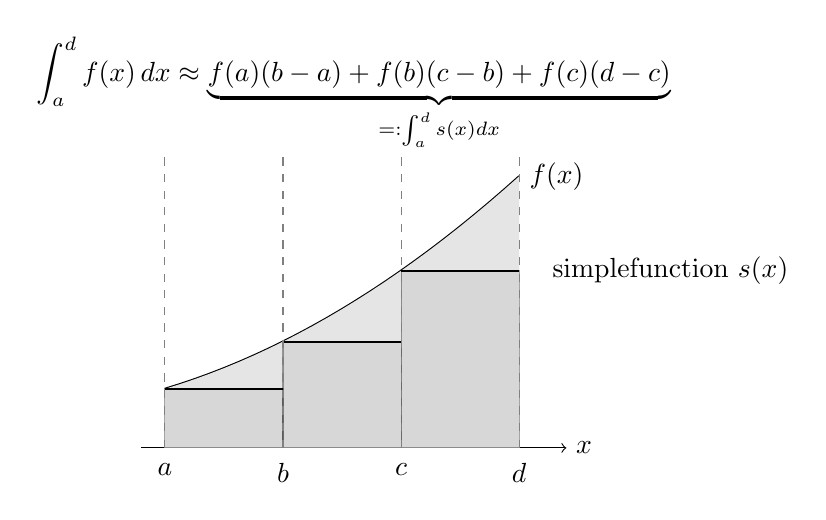
\begin{tikzpicture}[scale=1.5]
  			% Axes
  			\draw[->] (-0.2,0) -- (3.4,0) node[right] {$x$};
 			% \draw[->] (0,-0.1) -- (0,2.6) node[above] {$y$};
  			% Continuous function f(x)
  			\draw[thick,domain=0:3,smooth] plot(\x,{0.5+0.3*\x+0.1*\x*\x}) node[right] {$f(x)$};
  			% Shade area under f(x)
  			\fill[gray!20] (0,0) -- plot[domain=0:3] (\x,{0.5+0.3*\x+0.1*\x*\x}) -- (3,0) -- cycle;
  			% Lower simple function: left-endpoint rectangles for [0,1], [1,2], [2,3]
  			\draw[fill=gray!50,opacity=0.35] (0,0) rectangle (1,0.5);
  			%\node at (0.5,-0.2) {$\cluster^{(1)}$}; 
  			\draw[fill=gray!50,opacity=0.35] (1,0) rectangle (2,0.9);
  			\draw[fill=gray!50,opacity=0.35] (2,0) rectangle (3,1.5);
  			% Step lines of the simple function
  			\draw[thick] (0,0.5)--(1,0.5);
  			\draw[thick] (1,0.9)--(2,0.9);
  			\draw[thick] (2,1.5)--(3,1.5);
 	 		\node[above left] at (0.8,0.5) {};
  			% Dashed partition lines
  			\foreach \x in {0,1,2,3} \draw[dashed,gray] (\x,0) -- (\x,2.5);
  			% Labels
  			\node[anchor=north] at (0,-0.05) {$a$};
  			\node[anchor=north] at (1,-0.05) {$b$};
  			\node[anchor=north] at (2,-0.05) {$c$};
  			\node[anchor=north] at (3,-0.05) {$d$};
  			\node at (1.6,3.0) {$\displaystyle \int_a^d f(x)\,dx \approx \underbrace{f(a)(b-a) + f(b)(c-b)+f(c)(d-c)}_{=:\int_a^d s(x)dx}$};
  			\node [anchor=west] at (3.2,1.5) {\gls{simplefunction} $s(x)$};
			\end{tikzpicture}
		\end{figure}
 		It is useful to think of the Lebesgue integral as a \gls{function} that maps 
 		an \gls{integrable} \gls{function} $f$ to the value of its integral, 
		$$ f \mapsto \int_{\mathbb{R}^{\nrfeatures}} f(\featurevec) d\featurevec.$$ 
		The precise definition of this \gls{function}, whose \gls{domain} 
		consists of the \gls{integrable} \glspl{function}, is a cornerstone of 
		\gls{measure} theory \cite[Ch. 1]{RudinBook}.
					\\ 
		See also: \gls{function}.},
	first={Lebesgue integral},
	text={Lebesgue integral},
	type=math, 
	plural={Lebesgue integrals},
	firstplural={Lebesgue integrals}
}

\newglossaryentry{conditionalexpect}
{name={conditional expectation}, 
	description={Consider a numeric \gls{rv} $\featurevec \in \mathbb{R}^{\nrfeatures}$ defined on a 
                 \gls{probspace} $(\samplespace,\,\sigmaalgebra,\,\probmeasure)$. 
                 Let $\sigmaalgebra' \subseteq \sigmaalgebra$ be a (sub-)\gls{sigmaalgebra} that 
                 represents partial information about the \gls{outcome} of a \gls{randomexperiment}. 
                 The conditional \gls{expectation}\index{conditional expectation} of 
                 $\featurevec$ given (or conditioned on) $\sigmaalgebra'$, denoted 
                 $\expect\{ \featurevec \mid \sigmaalgebra'\}$, is a numeric \gls{rv} 
		that \cite{BillingsleyProbMeasure}, \cite{durrett2010probability}:
                	1) is \gls{measurable} with respect to $\sigmaalgebra'$; and
                 2) satisfies
		$$
    		\int_{\mathcal{A}} \expect\{\featurevec \mid \sigmaalgebra'\} {\rm d} \probmeasure =
    		\int_{\mathcal{A}} \featurevec {\rm d} \probmeasure \quad \text{for any } \mathcal{A} \in \sigmaalgebra'.
		$$
               	Intuitively, $\expect\{\featurevec \mid \sigmaalgebra'\}$ summarizes 
               	the average value of $\featurevec$ using only information contained 
               	in the (typically smaller) \gls{sigmaalgebra} $\sigmaalgebra'$ 
		\cite{BillingsleyProbMeasure}, \cite{GrayProbBook}, \cite{ross2013first}. 
		\\
              	See also: \gls{probspace}, \gls{sigmaalgebra}, \gls{expectation}.}, 
 	first={conditional expectation},
 	plural={conditional expectations}, 
 	type=math, 
 	firstplural={conditional expectations},  
 	text={conditional expectation}
}

\newglossaryentry{conditionalpmf}
{name={conditional probability mass function (conditional pmf)}, 
	description={Consider two \glspl{discreteRV} $\truelabel$ and $\feature$ defined on 
                 the same \gls{probspace} $(\samplespace,\,\eventspace,\,\prob{\cdot})$. 
                 The conditional \gls{pmf}\index{conditional probability mass function (conditional pmf)} 
                 of $\truelabel$ given (or conditioned on) $\feature$ is denoted by
		$\pmf{\truelabel \mid \feature}{\cdot \mid \cdot}$ and is defined by
                \[
                  \pmf{\truelabel \mid \feature}{\truelabel' \mid \feature'}
                  :=
                  \prob{\truelabel=\truelabel' \mid \feature=\feature'}
               \]
                for all \glspl{realization} $\truelabel',\feature'$ with 
                $\prob{\feature=\feature'}>0$. 
                Equivalently, the conditional \gls{pmf} can be expressed using 
                \gls{conditionalexpect} as
                \[
                  \pmf{\truelabel \mid \feature}{\truelabel' \mid \feature'}
                  =
                  \expect\{\indicatorfunc{\truelabel=\truelabel'}\mid \sigmaalgebra(\feature)\}(\feature')
                \]
                where $\sigmaalgebra(\feature)$ denotes the \gls{sigmaalgebra} generated by 
                the \gls{rv} $\feature$. 
                \\
              See also: \gls{probspace}, \gls{pmf}, \gls{conditionalexpect}.}, 
 	first={conditional probability mass function (conditional pmf)},
 	firstplural={conditional probability mass functions (conditional pmfs)}, 
 	type=math, 
 	plural={conditional pmfs},  
 	text={conditional pmf}
}

\newglossaryentry{iid}
{name={independent and identically distributed (i.i.d.)}, 
	description={A collection of \glspl{rv}\linebreak $\datapoint^{(1)}, \,\ldots, \,\datapoint^{(\samplesize)}$ 
            defined on the same \gls{probspace} $(\samplespace, \sigmaalgebra, \prob{\cdot})$ is 
		referred to as i.i.d.\index{independent and identically distributed (i.i.d.)} 
		if each $\datapoint^{(\sampleidx)}$ follows the same \gls{probdist}, and 
		the \glspl{rv} are mutually independent. That is, for any collection of 
		\glspl{event} $\mathcal{A}_1, \,\ldots, \,\mathcal{A}_\samplesize \in \sigmaalgebra$, we have
       		\[
          		\prob{ \datapoint^{(1)} \in \mathcal{A}_1, \,\ldots, \,\datapoint^{(\samplesize)} \in \mathcal{A}_{\samplesize}} 
         		= \prod_{\sampleidx=1}^{\samplesize} \prob{ \datapoint^{(\sampleidx)} \in \mathcal{A}_\sampleidx}.
         	\]
		Probability theory also guarantees the existence and construction of independent copies of \glspl{rv} 
            \cite[Theorem 2.19]{klenke2020probability}.\\
		See also: \gls{rv}, \gls{probdist}, \gls{event}, \gls{datapoint}, \gls{iidasspt}.},
	first={independent and identically distributed (i.i.d.)},
	type=math, 
	text={{i.i.d.}} 
}

\newglossaryentry{preimage}
{name={preimage}, 
	description={Consider a \gls{function}\index{preimage} $f\colon \mathcal{U} \rightarrow \mathcal{V}$ 
		between two sets. The preimage $f^{-1}(\mathcal{B})$ of a subset $\mathcal{B} \subseteq \mathcal{V}$ is the set 
		of all inputs $u \in \mathcal{U}$ that are mapped into $\mathcal{B}$ by $f$, i.e.,
		\[
		f^{-1}(\mathcal{B}) \defeq \{ u \in \mathcal{U} \mid f(u) \in \mathcal{B} \}.
		\]
		The preimage is well defined even if the \gls{function} $f$ is non-invertible \cite{RudinBookPrinciplesMatheAnalysis}.
		\\
		See also: \gls{function}. },
	first={preimage},
	type=math, 
	text={preimage}
}

\newglossaryentry{measurable}
{name={measurable}, 
	description={Consider\index{measurable} a \gls{randomexperiment}, such as recording 
		the air temperature at an \gls{fmi} weather station. The corresponding \gls{samplespace} 
		$\samplespace$ consists of all possible \glspl{outcome} $\outcome$ (e.g., 
		all possible temperature values in degree Celsius). In many \gls{ml} 
		applications, we are not interested in the exact \gls{outcome} $\outcome$, but only 
		whether it belongs to a subset $\mathcal{A} \subseteq \samplespace$ 
		(e.g., determining whether the temperature is below zero degrees). 
		We call such a subset $\mathcal{A}$ measurable if it is possible to 
		decide, for any \gls{outcome} $\outcome$, whether $\outcome \in \mathcal{A}$ 
		or not (see Fig.\ \ref{fig_measurable_dict}). \\
		\begin{figure}[H]
		\begin{center}
		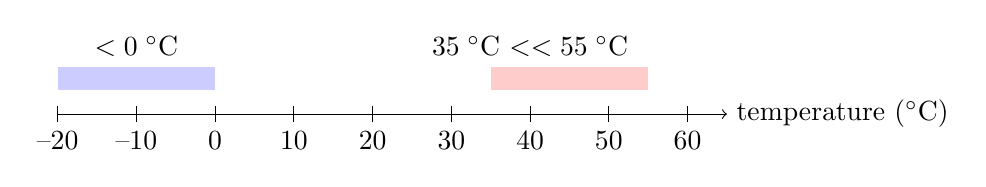
\begin{tikzpicture}
			% Draw temperature axis
			\draw[->] (0,0) -- (8.5,0) node[right] {temperature ($^\circ$C)};
			% Add tick marks and labels every 20 degrees from -20 to 100
			\foreach \x/\label in {0/--20, 1/--10, 2/0, 3/10, 4/20, 5/30, 6/40, 7/50, 8/60} {
			\draw (\x,0.1) -- (\x,-0.1);
			\node[below] at (\x,-0.1) {\label};
			}
			% Shade measurable set: Temperature < 0°C
			\fill[blue!20] (0,0.3) rectangle (2,0.6);
			\node[above] at (1,0.6) {$\outcome < 0\;^\circ$C};
			% Shade measurable set: 5°C < omega < 10°C
			\fill[red!20] (5.5,0.3) rectangle (7.5,0.6);
			\node[above] at (6,0.6) {$35\;^\circ$C $< \outcome < 55\;^\circ$C};
			\vspace*{10mm}
			\end{tikzpicture}
			\vspace*{10mm}
			\end{center}
			\caption{A \gls{samplespace} constituted by all possible temperature values $\outcome$ 
			that can occur at an \gls{fmi} station. Two measurable subsets of temperature 
			values, denoted by $\mathcal{A}^{(1)}$ and $\mathcal{A}^{(2)}$, are highlighted. For any 
			actual temperature value $\outcome$, it is possible to determine (via some equipment) 
			whether $\outcome \in \mathcal{A}^{(1)}$ and whether $\outcome \in \mathcal{A}^{(2)}$. 
			\label{fig_measurable_dict}} 
		\end{figure}
		In principle, measurable sets could be chosen freely (e.g., depending on the resolution of the 
		measuring equipment). However, it is often useful to impose certain completeness requirements 
		on the collection of measurable sets. For example, the \gls{samplespace} itself should be 
		measurable, and the union of two measurable sets should also be measurable. These completeness 
		requirements can be formalized via the concept of a \gls{sigmaalgebra} (or \gls{sigmafield}) 
		\cite{RudinBook}, \cite{BillingsleyProbMeasure}, \cite{durrett2010probability}. 
		A measurable space is a pair $\big(\featurespace,\eventspace\big)$ that consists of an arbitrary 
		set $\featurespace$ and a collection $\eventspace$ of measurable subsets of $\featurespace$ 
		that form a \gls{sigmaalgebra}. 
		\\
		See also: \gls{samplespace}, \gls{outcome}, \gls{sigmaalgebra}, \gls{probability}.},
	first={measurable},
	type=math, 
	text={measurable} 
}

\newglossaryentry{sigmaalgebra}
{name={$\sigma$-algebra}, 
sort={sigma-algebra},
	description={Consider a \gls{randomexperiment} with a \gls{samplespace} $\samplespace$. 
		A $\sigma$-algebra\index{$\sigma$-algebra} (or \gls{sigmafield}) $\sigmaalgebra$ 
		is a collection of subsets of $\samplespace$ with the following properties 
		\cite{RudinBook}, \cite{BillingsleyProbMeasure}, \cite{durrett2010probability}:
		\begin{itemize}
		 	\item The empty set $\emptyset$ and the entire \gls{samplespace} 
		 	$\samplespace$ belong to $\sigmaalgebra$, i.e., $\emptyset \in \sigmaalgebra$ and $\samplespace \in \sigmaalgebra$.
		 	\item If a set $\mathcal{A}$ belongs to $\sigmaalgebra$, then its complement 
		 	$\samplespace \setminus \mathcal{A}$ also belongs to $\sigmaalgebra$, i.e., 
		 	$\mathcal{A} \in \sigmaalgebra$ implies $\samplespace \setminus \mathcal{A} \in \sigmaalgebra$.
		 	\item If a \gls{countable} collection of sets $\mathcal{A}_1, \,\mathcal{A}_2, \,\ldots$ belongs 
			to $\sigmaalgebra$, 
		 	then their union also belongs to $\sigmaalgebra$, i.e.,
		 	$\mathcal{A}_1, \,\mathcal{A}_2, \,\ldots \in \sigmaalgebra$ implies 
		 	$\bigcup_{i=1}^{\infty} \mathcal{A}_i \in \sigmaalgebra$.	
		 \end{itemize}			 
		See also: \gls{samplespace}, \gls{rv}, \gls{probspace}.},
	first={$\sigma$-algebra},
	type=math, 
	text={$\sigma$-algebra} 
}

\newglossaryentry{sigmafield}
{name={$\sigma$-field}, 
sort={sigma-field},
	description={See \gls{sigmaalgebra}\index{$\sigma$-field}.}, 
	first={$\sigma$-field},
	type=math,
	text={$\sigma$-field} 
}

\newglossaryentry{injective}
{name={injective}, 
	description={A \gls{function} $f: \mathcal{U} \rightarrow \mathcal{V}$ is injective\index{injective} 
		if it maps distinct elements of its \gls{domain} to distinct elements 
		of its \gls{co-domain}, 
    		i.e., if $f(u_1) = f(u_2)$ implies $u_1 = u_2$ for all $u_1, u_2 \in \mathcal{U}$ 
        		\cite{HalmosSet}. 
    		Equivalently, no two different \gls{function} inputs are mapped to the same \gls{function} \gls{output}.
				\\
		See also: \gls{function}.},
	first={injective},
	type=math,
	text={injective} 
}

\newglossaryentry{typicalset}
{name={typical set}, 
	description={See \gls{pmf}\index{typical set}.}, 
 	first={typical set},
 	firstplural={typical sets},
 	type=math,
 	plural={typical sets},
 	text={typical set} 
}

\newglossaryentry{majmin}
{name={majorize-minimize (MM)}, 
	description={Consider an \gls{optproblem} $\min_{\weights \in \paramspace} f(\weights)$ with 
		some complicated (potentially non-\gls{convex} and \gls{nonsmooth}) \gls{objfunc}. 
		One important example of such an \gls{optproblem} is \gls{erm}, which is used to learn the 
		\glspl{modelparam} of a nonlinear \gls{model}. 
		An MM method is\index{majorize-minimize (MM)} an iterative \gls{optmethod} 
		that constructs a \gls{sequence} $\weights^{(1)},\,\weights^{(2)},\,\ldots \in \paramspace$ 
		of \glspl{modelparam} as follows \cite{Lange2016MM}, \cite{BishopBook}, \cite{Hunter01022004}
		(see also Fig. \ref{fig:majmin_dict}): 
		\begin{itemize} 
			\item During the $\iteridx$th \gls{iteration}, the \gls{objfunc} $f(\cdot)$ 
			 	is approximated by another \gls{function} $g\big(\cdot;\weights^{(\iteridx)}\big)$.
	             	  	This approximation must be an upper bound for (i.e., must majorize) the original
				\gls{objfunc}, i.e., $g\big(\weights;\weights^{(\iteridx)}\big) \geq f(\weights)$ 
			 	for all $\weights \in \paramspace$, and it must be tight for $\weights^{(\iteridx)}$, i.e., 
			 	$g\big(\weights^{(\iteridx)};\weights^{(\iteridx)}\big) = f\big(\weights^{(\iteridx)}\big)$.
			\item The new \glspl{modelparam}  $\weights^{(\iteridx+1)}$ are then obtained by 
				minimizing the approximation, i.e., 
				 $\weights^{(\iteridx+1)} \in \argmin_{\weights \in \paramspace}g\big(\weights;\weights^{(\iteridx)}\big)$. 
		\end{itemize} 
		\begin{figure}[H]
			 \centering
			 \begin{tikzpicture}[x=1.2cm,y=1cm]
				% --- parameters ---
				\def\xa{0}
				\def\xb{2*pi}
				\def\xo{3*pi/4}     % touch point: 1.5 * (pi/2) = 3pi/4
				\def\mL{0.4}        % left slope  (adjust to keep it above the sine)
				\def\mR{0.7}        % right slope (adjust to keep it above the sine)
				% horizontal axis
				\draw[->] (\xa-0.2,-2) -- (\xb+0.3,-2) node[right] {$\weights$};
				% sine over one period
				\draw[thick,samples=100,domain=\xa:\xb]
				plot (\x,{sin(\x r)}) node[pos=0.1,above left,black] {\small $f(\weights)$};
				% compute y0 = sin(w0)
				\pgfmathsetmacro\yxo{sin(\xo r)}
				% Anchors (numeric, no macros)
				% w0 = 3*pi/4 = 2.35619449
				% xL = 2.00619449, xR = 2.70619449
				% y0 = sin(w0) = 0.70710678
				% Left slope mL = cos(xL) = -0.42177145  (tangent => upper bound on [0, xL])
				% Right slope mR = 0.7  (rising; safely above the sine on [xR, 2*pi])
				\def\xL{2.70}
				\def\xR{3.80}
				\def\yO{0.70}
				% Left (tangent) segment: y = y0 + mL*(x - xL), mL = -0.42177145
				\draw[dashed,samples=2,domain=0:\xL]
				plot (\x,{\yO + (-0.7)*(\x - \xo)});
				% Flat touching segment
				\draw[dashed]
				(\xL,{\yO+(-0.7)*(\xL-\xo)}) -- (\xR,{\yO+(-0.7)*(\xL-\xo)});
				% Right rising segment: y = y0 + mR*(x - xR), mR = 0.7
				% draw the segment
				\draw[dashed,samples=2,domain=\xR:2*pi]
				plot (\x,{\yO+(-0.7)*(\xL-\xo) + (0.7)*(\x - \xR)});
				% compute a point 65% along the x-range [\xR, 2*pi]
				\pgfmathparse{\xR + 0.65*(2*pi - \xR)} \let\xmid\pgfmathresult
				\pgfmathparse{\yO + 0.7*(\xmid - \xR)} \let\ymid\pgfmathresult
				% label at that point
				\node[right,black] at (\xmid,\ymid) {$g\big( \weights; \weights^{(\iteridx)} \big)$};
				% Touch marker at w0
				\fill[red] (2.35619449,0.70710678) circle (1.2pt);
				% --- vertical ruler marking w0 ---
				\draw[densely dotted,gray] (\xo,-2) -- (\xo,\yO);
				% \draw[gray] (\xo,0) -- ++(0,-2.06);
				\node[below] at (\xo,-2) {$\weights^{(\iteridx)}$};
			\end{tikzpicture}
		\caption{The construction of \glspl{modelparam} based on the iterative MM method.}
			\label{fig:majmin_dict}
		\end{figure}
		Similar to \glspl{gdmethod}, the MM principle is also based on approximating an 
		\gls{objfunc} locally, around the current \glspl{modelparam}, and then optimizing 
		this approximation to obtain new \glspl{modelparam}. However, the construction 
		of local approximations is very different. While \glspl{gdmethod} use linear \glspl{function} 
		for these approximations, MM methods can use nonlinear \glspl{function} as long as 
		they are upper bounds for the original \gls{objfunc}. 
			 \\ 
		See also: \gls{gdmethod}, \gls{em}.},
	first={majorize–minimize (MM)},
	type=math, 
	text={MM}
}

\newglossaryentry{markovsinequality}
{name={Markov's inequality},
	description={Consider a real-valued nonnegative \gls{rv} $x$ for which 
		the \gls{expectation} $\expect\{ x\}$ exists. \index{Markov's inequality} 
	 	Markov's inequality provides an upper bound on the \gls{probability} 
	 	$\prob{x\geq a}$ that $x$ exceeds a given positive threshold $a>0$.  
	 	In particular,          
	 	\begin{equation}
            		\nonumber
			\prob{x \geq a} \leq \frac{\expect \{ x\}}{a} \qquad \mbox{ holds for any } a > 0. 
            		%\label{eq:markovsinequality_dict}
    		\end{equation}
    		This inequality can be verified by noting that $\prob{x \geq a}$ is the 
		\gls{expectation} $\expect\{g(x)\}$ with the \gls{function} 
	 	$$g: \mathbb{R} \rightarrow \mathbb{R}: x' \mapsto \indicatorfunc{\{x \geq a\}}(x').$$ 
	 	As illustrated in Fig. \ref{fig:markovsinequality_dict}, for any positive $a>0$, 
	 	$$ g(x') \leq x'/a \mbox{ for all } x' \in \mathbb{R}.$$ 
	 	This implies Markov's inequality via the monotonicity property 
	 	of the \gls{LebesgueIntegral} \cite[p. 50]{folland1999real}. 
    		\begin{figure}[H]
			\centering
			\begin{tikzpicture}[scale=1, x=0.8cm, y=0.8cm]
			% -------- parameters ----------
			\def\a{3.24}      % threshold a
			\def\xmax{10}     % x-axis max
			\def\m{0.02}      % slope of the linear function y = m(x-a)+1
			% -------- pdf function p(x) (same as your expression) ----------
			% p(x) = (1/(3*sqrt(2*pi))) * x^(1.5) * exp(-x/2)
			\draw[-{Latex}] (0,0) -- (\xmax+1,0) node[below right] {$x'$};
			%\draw[-{Latex}] (0,0) -- (0,3.1) node[left] {$\pdf{x}{x'}$};
                		\draw[-{Latex}] (0,0) -- (0,3.1)  node[left, text=blue!70!black] {$\pdf{x}{x'}$};
			% Fill under the pdf (optional aesthetics)
			\fill[blue!15, opacity=0.3]
			plot[samples=400, domain=0:\xmax, smooth]
			(\x,{ (6/sqrt(2*pi)) * (\x)^(1.5) * exp(-\x/2) }) -- (\xmax,0) -- (0,0) -- cycle;
			% PDF curve
			\draw[blue!70!black, very thick, samples=400, domain=0:\xmax, smooth]
			plot (\x,{ (6/(sqrt(2*pi))) * (\x)^(1.5) * exp(-\x/2) })
			node[pos=0.9, above right, xshift=2pt] {};
			% Vertical guide at x=a
			\draw[dashed, gray] (\a,0) -- (\a,1.05);
			\node[below] at (\a,0) {$a$};
			\node[above] at (1*\a,3) {$\prob{x \geq a} \leq \frac{\expect \{ x\}}{a}$}; 
			\node[below] at (0,0) {$0$};
			% -------- indicator 1{x >= a} ----------
			% 0 for x<a with open circle at (a,0)
			\draw[green!60!black, ultra thick] (0,0) -- (\a,0);
			\filldraw[white, draw=green!60!black, line width=0.8pt] (\a,0) circle (2pt);
			% 1 for x>=a with closed circle at (a,1)
			\draw[green!60!black, ultra thick] (\a,1) -- (\xmax,1)
			node[pos=0.9, above, yshift=2pt] {$\indicatorfunc{\{x \ge a\}}(x')$};
			\filldraw[green!60!black] (\a,1) circle (2pt);
			% -------- linear curve through (a,1): y = m(x-a)+1 ----------
			\draw[red!70, very thick, samples=2, domain=0:\xmax]
			plot (\x,{ \x*(1/\a) }); 
			\node[align=right,red!70,yshift=20pt] at ({2.5*\a+0.2},{2.5}) {$f(x') = x'/a$};  
			% Axis marker for y=1
			\draw (0,1) -- ++(-0.12,0) node[left] {$1$};
			\end{tikzpicture}
            	\caption{The \gls{expectation} $\expect\{x\}$ and the \gls{probability} $\prob{x \geq a}$ 
			of a nonnegative \gls{rv} $x$ with a \gls{pdf} $\pdf{x}{\cdot}$           
                		%a \gls{probdist} $\probdist^{(x)}$ 
			can be obtained via \glspl{LebesgueIntegral} of 
			$f(x') = x'/a$ and $g(x') = \indicatorfunc{\{x \geq a\}}(x')$, respectively.}
            		\label{fig:markovsinequality_dict}
        		\end{figure} 
		See also: \gls{expectation}, \gls{probability}, \gls{concentrationinequ}.},
	first={Markov's inequality},
	type=math, 
    	text={Markov's inequality}  
}

\newglossaryentry{chebyshevsinequality}
{name={Chebyshev's inequality},
	description={Consider a real-valued \gls{rv} $x$ for which 
		the second moment $\expect\{ x^{2} \}$ exists (and is finite). 
 	 	The existence of the second moment implies the existence 
 	 	of a finite \gls{expectation} $\mu \defeq \expect\{ x\}$ and a finite 
 	 	\gls{variance} $\sigma^{2}\!\defeq\!\expect \big\{ \big( x\!-\!\mu \big)^{2} \big\}$ \cite[Proposition 6.12]{folland1999real}. 
 	 	Chebyshev's inequality\index{Chebyshev's inequality} refers 
 	 	to the following upper bound on the \gls{probability} that $x$ 
 	 	deviates from $\mu$ by more than a given threshold $\eta$ 
 	 	\cite[Ch. 4]{FellerBook}. 
 	 	In particular,   
 		\begin{equation}
           		\nonumber
			\prob{\big|x - \mu \big| \geq \eta } \leq \frac{\sigma^2}{\eta^2} \qquad \mbox{ for any } \eta > 0.
            		%\label{eq:chebyshevsinequality_dict}
     		\end{equation}
 		This upper bound can be obtained by applying \gls{markovsinequality} to 
 		the new \gls{rv} $\tilde{x}\!\defeq\! \big(x\!-\!\mu \big)^2$. 
  		\begin{figure}[H]
   			\centering
			\begin{tikzpicture}
     			\begin{axis}[
      			width=9cm, height=4.2cm,
      			samples=300,
      			axis lines=left,
	  		ylabel={$\pdf{x}{x'}$},
      			xlabel={$x'$},
      			x label style={at={(axis description cs:1,0)}, anchor=west},
	  		ylabel style={rotate=270,anchor=south,at={(axis description cs:0,1.02)}},
      			xtick={-1.5,0,1.5},
      			xticklabels={$-\eta$,$\mu$,$\eta$},
      			ytick=\empty,
      			ymin=0, ymax=0.45,
      			domain=-4:4,
      			clip=false
    			]
      			% pdf (centered at mu; here shown as standard normal in x - mu coordinates)
      			\addplot[name path=pdf, black, very thick] {exp(-0.5*x^2)/sqrt(2*pi)};
      			\addplot[name path=axis, draw=none] {0};
      			% shaded tails: |X - mu| >= t with t = 1.5
      			\addplot[red!70, opacity=0.25] fill between[of=pdf and axis, soft clip={domain=1.5:4}];
      			\addplot[red!70, opacity=0.25] fill between[of=pdf and axis, soft clip={domain=-4:-1.5}];
      			% guide lines at mu and ±t
      			\draw[densely dashed] (axis cs:0,0) -- (axis cs:0,0.42);
      			\draw[dashed] (axis cs:1.5,0) -- (axis cs:1.5,{exp(-0.5*1.5^2)/sqrt(2*pi)});
      			\draw[dashed] (axis cs:-1.5,0) -- (axis cs:-1.5,{exp(-0.5*1.5^2)/sqrt(2*pi)});
      			% label for the shaded area
   			%   \node[anchor=west] at (axis description cs:0.72,0.82) {$\prob{|x-\mu|\ge \eta}$};
    			\end{axis}
  			\end{tikzpicture}
  		\caption{Chebyshev's inquality provides an upper bound on 
              		the tail \gls{probability} $\prob{|x-\mu|\ge \eta}$ (i.e., shaded area) of
			a real-valued \gls{rv} $x$ with a finite second moment.\label{fig:chebyshev_minimal_dict}} 
		\end{figure}
     		See also: \gls{expectation}, \gls{markovsinequality}, \gls{concentrationinequ}.},
    	first={Chebyshev's inequality},
	type=math, 
     	text={Chebyshev's inequality}  
}

\newglossaryentry{hoeffdingsinequality}
{name={Hoeffding's inequality},
	description={\index{Hoeffding's inequality} Hoeffding's inequality \cite{Hoeffding1963} is a fundamental \gls{concentrationinequ} 
		that provides an upper bound on the \gls{probability} that a sum (or average) of independent, bounded \glspl{rv} 
		deviates from its \gls{mean} by more than some threshold. 
     		Let $x_1,\,\dots,\,x_n$ be independent real-valued \glspl{rv} $x_i$ taking values in $[a_i,b_i] \subset \mathbb{R}$, 
		and $S_n \defeq \sum_{i=1}^n x_i$ and $\expect\{S_n\} = \sum_{i=1}^n \expect\{x_i\}$. 
		Then, Hoeffding's inequality \cite[Th. 2.2.6]{vershynin2018high} states that
        		\begin{equation}
                		\nonumber
			\prob{ |S_n - \expect\{S_n\}| \geq t } 
            		\leq 2 \exp \left( -\frac{2 t^2}{\sum\limits_{i=1}^n (b_i - a_i)^2} \right) \qquad \forall t > 0.
            		%\label{eq:hoeffding_sum}
        		\end{equation}
    		Hoeffding's inequality typically provides sharper bounds than \gls{chebyshevsinequality}, 
		but it is more restrictive by assuming bounded \glspl{rv}.
    		In the context of \gls{ml}, this result is useful for deriving guarantees for \gls{erm}  and in the context of \gls{mab}. 
		 \\
    		See also: \gls{concentrationinequ}, \gls{probability}, \gls{rv}, \gls{chebyshevsinequality}, \gls{expectation}, \gls{probspace}, \gls{markovsinequality}.},
    	first={Hoeffding's inequality},
	type=math, 
    	text={Hoeffding's inequality}  
}

\newglossaryentry{rgg}
{name={random geometric graph (RGG)},
	description={An RGG\index{random geometric graph (RGG)} is a \gls{probmodel} for \glspl{graph} 
		built from nodes randomly placed in a \gls{metricspace}. Given a \gls{metricspace}, the RGG is characterized by 
		the number of nodes, the connection radius, and the \gls{probdist} describing the node placement. 
    		More precisely, for a node set $\nodeidx=1, \,\ldots, \,\nrnodes$, each node $\nodeidx$ is assigned to a random position 
		$\featurevec^{(\nodeidx)} \in \featurespace$, typically as \glspl{realization} of \gls{iid} \glspl{rv} taking values in a set $\featurespace$. 
		Together with a \gls{metric}, this forms a \gls{metricspace}, often with the \gls{metric} induced by a \gls{norm}. 
		A specific \gls{realization} of an RGG contains an edge $\edge{\nodeidx}{\nodeidx'}$ if and only if the distance between the nodes 
		with respect to the \gls{metric} is smaller than some threshold, i.e., when $\metric{\featurevec^{(\nodeidx)}}{\featurevec^{(\nodeidx')}}\leq r$ 
		for some threshold $r>0$, as illustrated in Fig. \ref{fig:rgg}.
         	\begin{figure}[H]
    			\centering
    			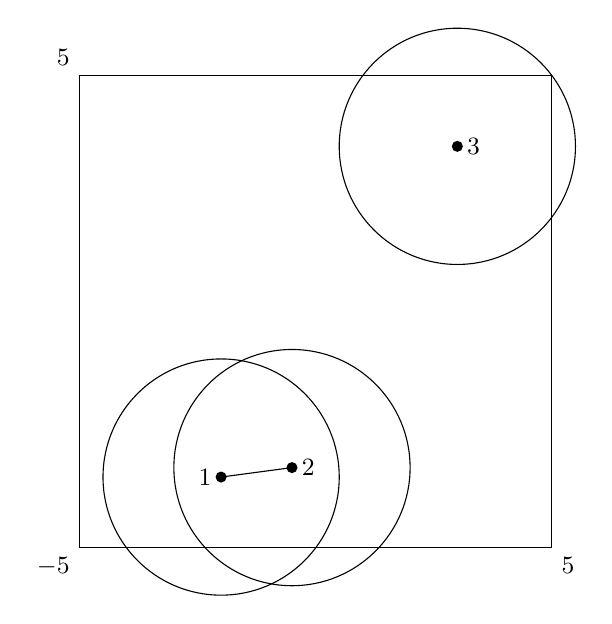
\begin{tikzpicture}[x=0.6cm,y=0.6cm]
        				\draw (-5,-5) rectangle (5,5);
        				% Corner labels outside the rectangle
        				\node[below left] at (-5,-5) {\small $-5$};
        				\node[above left]  at (-5, 5) {\small $5$};
        				\node[below right] at ( 5,-5) {\small $5$};
        				% Bottom two points (nodes 1 and 2) within each other's circle of radius 2.5
        				\fill (-2.0,-3.5) circle (2pt);
        				\draw (-2.0,-3.5) circle (2.5);
        				\node[anchor=east] at (-2.0,-3.5) {\small 1};
        				\fill (-0.5,-3.3) circle (2pt);
        				\draw (-0.5,-3.3) circle (2.5);
        				\node[anchor=west] at (-0.5,-3.3) {\small 2};
        				\draw (-2.0,-3.5) -- (-0.5,-3.3);
        				% Top point (node 3) outside the bottom circles
        				\fill (3.0,3.5) circle (2pt);
        				\draw (3.0,3.5) circle (2.5);
        				\node[anchor=west] at (3.0,3.5) {\small 3};
    			\end{tikzpicture}
   		\caption{Illustration of an RGG with $ \featurespace = [-5,5]\times[-5,5] \subset \mathbb{R}^2$ and radius $r=2.5$ 
			(with respect to the \gls{eucliddist}), where nodes 1 and 2 (corresponding to $(-2.0, -3.5)^T$ and $(-0.5, -3.3)^T$, 
			within radius $r=2.5$) are connected, while node 3 (corresponding to $(3.0, 3.5)^T$) has no other node within that distance.}
    			\label{fig:rgg}
    		\end{figure}
        		See also: \gls{graph}, \gls{sbm}, \gls{ergraph}.},
    	first={random geometric graph (RGG)},
	type=math, 
    	text={RGG}
}

\newglossaryentry{banachfixedpoint}
{name={Banach's fixed-point theorem},
	description={Banach's fixed-point theorem\index{Banach's fixed-point 
		theorem} (also referred to as the contraction principle \cite[Th. 9.23]{RudinBookPrinciplesMatheAnalysis},\cite{Kelley1995}) 
		states that every \gls{contractop} $\fixedpointop$ on a complete 
		\gls{metricspace} $\paramspace$ has a unique \gls{fixedpoint}. 
		Formally, let $(\paramspace,\metric{\cdot}{\cdot})$ be a non-empty 
		complete \gls{metricspace} and let $\fixedpointop:\paramspace\to\paramspace$ satisfy
    		\[
    		\metric{\fixedpointop \weights}{\fixedpointop \weights'} \leq \contractfac \cdot \metric{\weights}{\weights'} \qquad \forall \weights,\weights'\in\paramspace
    		\]
    		for some constant $\contractfac \in [0,1)$. Then, $\fixedpointop$ has a unique \gls{fixedpoint}, 
		i.e., there exists a unique $\weights^\star\in\paramspace$ with 
		$\fixedpointop \weights^\star =\weights^\star$. Moreover, for any initial 
		$\weights^{(0)}\in\paramspace$, the \gls{fixedpointiter} 
		$\weights^{(\iteridx)}\!=\!\fixedpointop \weights^{(\iteridx-1)}$, for $\iteridx=1,\,2,\,\dots$, 
		converges to $\weights^\star$ at a rate governed by $\contractfac$. 
		In particular, 
		\[ \metric{\weights^{(\iteridx)}}{\weights^\star} \leq \contractfac^{\iteridx}
		 \cdot \metric{\weights^{(0)}}{\weights^\star} \mbox{, for }\iteridx=1,\,2,\,\dots. \]   		
		\begin{figure}[H]
    			\centering
    			\begin{tikzpicture}[>=Latex, font=\small]
    			\tikzset{space/.style={draw, thick, circle, minimum size=4.0cm},pt/.style={circle, inner sep=1.5pt, draw, fill=black},maparrow/.style={->, very thick},link/.style={->, thick},distline/.style={dashed, thick}}
    			\def\dx{6.5}
    			\node[space,label=above:{$\paramspace$}] (XL) at (0,0) {};
    			\node[space,label=above:{$\paramspace$}] (XR) at (\dx,0) {};
    			\draw[maparrow] (XL.east) -- node[above=2pt] {$\fixedpointop$} (XR.west);
    			\coordinate (x1) at (-0.8,0.9);
    			\coordinate (x2) at (0.9,0.5);
    			\node[pt,label=above left:{$\weights$}] at (x1) {};
    			\node[pt,label=right:{$\weights'$}] at (x2) {};
    			\coordinate (fx1) at (\dx-0.3,0.5);
    			\coordinate (fx2) at (\dx+0.6,0.5);
    			\node[pt] (FX1) at (fx1) {};
    			\node[pt] (FX2) at (fx2) {};
    			\node[anchor=east] at ($(FX1.west)+(-6pt,-2pt)$) {$\fixedpointop \weights$};
    			\node[anchor=west] at ($(FX2.east)+(6pt,-2pt)$) {$\fixedpointop \weights'$};
   			% \draw[distline] (x1) -- (x2) node[midway, above=6pt, sloped] {$\metric{\fixedpointop \weights}{\fixedpointop \weights'}$};
   			% \draw[distline] (fx1) -- (fx2) node[midway, above=6pt, sloped] {$\metric{\weights}{\weights'}$};
    			\coordinate (xsL) at (0,-0.9);
    			\coordinate (xsR) at (\dx,-0.9);
    			\node[pt,label=below:{$\weights^\star$}] at (xsL) {};
    			\node[pt,label=below:{$\fixedpointop \weights^\star\!=\!\weights^\star$}] at (xsR) {};
    			\end{tikzpicture}
   	 	\caption{A \gls{contractop} $\fixedpointop:\paramspace\to\paramspace$  
	  		has a unique \gls{fixedpoint} $\weights^\star$ with 
			$\fixedpointop \weights^\star\!=\!\weights^\star$.}
    			\label{fig:banach_dict}
    		\end{figure}
    		See also: \gls{contractop}, \gls{fixedpointiter}.},
    	first={Banach's fixed-point theorem},
	text={Banach's fixed-point theorem},
    	type=math
}

\newglossaryentry{cvxoptproblem}
{name={convex optimization problem}, 
	description={See\index{convex optimization problem} \gls{convexopt}.},
	first={convex optimization problem},
	firstplural={convex optimization problems}, 
	type=math,
	plural={convex optimization problems}, 
	text={convex optimization problem}
}

\newglossaryentry{optimization}
{name={optimization}, 
	description={See\index{optimization} \gls{convexopt}, \gls{optmethod}, \gls{optproblem}.},
	first={optimization},
	firstplural={optimizations}, 
	type=math,
	plural={optimizations}, 
	text={optimization}
}

\newglossaryentry{optproblem}
{name={optimization problem}, 
	description={An\index{optimization problem} optimization problem is a mathematical 
		   structure consisting of an \gls{objfunc} $f: \mathcal{U} \rightarrow \mathcal{V}$ 
		   defined over an optimization variable $\weights \in \mathcal{U}$, together with a 
		   feasible set $\paramspace \subseteq \mathcal{U}$. The \gls{co-domain} $\mathcal{V}$ is 
		   assumed to be ordered, meaning that for any two elements $\mathbf{a}, \mathbf{b} \in \mathcal{V}$, 
		   we can determine whether $\mathbf{a} \leq \mathbf{b}$.
		   Here, ``$\leq$'' denotes a general partial order relation, which may differ from the standard 
		   numerical order on real numbers \cite[Sec. 2.4]{BoydConvexBook}. 
		   The goal in optimization is to find those values $\weights \in \paramspace$ 
		   for which the objective $f(\weights)$ is extremal—i.e., minimal or maximal 
		   \cite{BoydConvexBook}, \cite{BertsekasNonLinProgr}, \cite{nesterov04}.
		   \\
		   See also: \gls{objfunc}.},
	first={optimization problem},
	firstplural={optimization problems}, 
	type=math,
	plural={optimization problems}, 
	text={optimization problem}
}

\newglossaryentry{optmethod}
{name={optimization method},
	description={An\index{optimization method} optimization method is 
		an \gls{algorithm} that takes a representation of an 
		\gls{optproblem} as input and computes an (approximate) 
		solution as its \gls{output}. A central example of an \gls{optproblem} 
		in \gls{ml} is \gls{erm}. By applying an appropriate 
		optimization method to \gls{erm}, we obtain a concrete learning 
		\gls{algorithm} \cite{BoydConvexBook}, \cite{BertsekasNonLinProgr},
		\cite{nesterov04}.
		 \\
		 See also: \gls{algorithm}, \gls{optproblem}.},
	type=math, 
	first={optimization method},
	firstplural={optimization methods}, 
	plural={optimization methods}, 
	text={optimization method}
}

\newglossaryentry{convexopt}
{name={convex optimization},
 	description={\Gls{convex} optimization\index{convex optimization} studies the 
		formulation, properties, and efficient solution methods for \gls{convex} \glspl{optproblem} \cite{BoydConvexBook}.  
		A \gls{convex} \gls{optproblem} (defined on the \gls{euclidspace} $\mathbb{R}^{\nrfeatures}$) 
		consists of a \gls{convex} \gls{objfunc} $f: \mathbb{R}^{\nrfeatures} \rightarrow \mathbb{R}$  
    		and a \gls{convex} constraint set $\mathcal{C}$ for the optimization variable $\weights$.  
    		It can be written compactly as \cite{BoydConvexBook}
		$$ \min_{\weights \in \mathcal{C}}  f(\weights).$$ 
		Alternatively, a \gls{convex} \gls{optproblem} can be expressed in 
		terms of \gls{convex} constraint \glspl{function} $g_1,\,\ldots,\,g_k$ as
		\begin{align} 
			\min_{\weights \in \mathbb{R}^{\nrfeatures}} & f(\weights)   \nonumber \\ 
			\mbox{s.t.} \quad & g_{\sampleidx}(\weights) \leq 0, \quad \sampleidx=1,\,\ldots,\,k. \label{equ_def_convx_opt_constr_dict}
		\end{align} 
		\begin{figure}[H]
			\centering
			\begin{tikzpicture}[>=stealth, scale=1.0]
  			% Axes
  			\draw[->] (-3,0) -- (5.2,0) node[below] {$\vc$};
  			\draw[->] (0,-0.2) -- (0,4.2) node[left] {$t$};
  			% Exponential boundary: t = 3 e^{-g}
  			\draw[thick, domain=-1:3, smooth, variable=\x, name path=boundary]
    			plot ({\x},{exp(-\x)});%node[pos=0.45, below right] {};
  			% Transparent epigraph region (above the curve)
  			\path[fill=gray!40, opacity=0.4]
    			(-1,3) -- (-1,{exp(1)}) -- plot[domain=-1:3] ({\x},{exp(-\x)})
   			-- (3,3) -- cycle;
  			% Crossing with vertical axis (g=0): mark and label f^*
  			\fill (0,1) circle (1.6pt) node[left] {$f^{\ast}$};
  			% Tangent at g=1: slope = -e^{-1}, passes through (1, e^{-1})
  			% Equation: t = (2/e) - (1/e) * g
  			\draw[dashed, domain=-1:3, smooth, variable=\x]
    			plot ({\x},{(2/exp(1)) - (1/exp(1))*\x}); 
   			% node[pos=0.15, above right] {tangent at $g=1$};
  			% (Optional) mark the point of tangency
  			\fill (1,{1/exp(1)}) circle (1.2pt);
  			% Label for shaded region
  			\node at (2.6,2.5) {$\mathcal{A}$};
  			\node [below,yshift=-3pt] at (0,-0.2) {$\mathbf{0}$};
  			\end{tikzpicture}
  		\caption{A \gls{convex} \gls{optproblem} \eqref{equ_def_convx_opt_constr_dict} can be represented 
  			by a set $\mathcal{A}$ that consists of objective values $t$ and constraint values 
  			$\vc=\big(c_{1},\,\ldots,\,c_{\nrfeatures}\big)^{T}$ that are achievable, i.e., 
  			$f(\weights) \leq t, g_{1}(\weights)\leq c_{1},\,\ldots, \,g_{k}(\weights) \leq c_{k}$ 
  			for some $\weights \in \mathbb{R}^{\nrfeatures}$. The optimal value $f^{\ast}$ of the 
  			\gls{optproblem} is the smallest $t$ for which $(\mathbf{0},t) \in \mathcal{A}$. }
		\end{figure}
		The formulation \eqref{equ_def_convx_opt_constr_dict} lends, in turn, to the 
		\gls{epigraph} form of \cite[Sec. 5.3]{BoydConvexBook} 
		$$\inf \big\{ t \in \mathbb{R} : (\mathbf{0}, t) \in \mathcal{A} \big\}$$ 
		with the set 
		\begin{align} 
			\mathcal{A} \defeq 
    			\big\{ (\vc,t) & \in \mathbb{R}^{\nrfeatures} \times \mathbb{R} : 
    			f(\weights) \leq t, \, \nonumber \\ 
   			&  g_{\sampleidx}(\weights) \leq c_{\sampleidx}, \,
    			\sampleidx = 1,\,\ldots,\,k, 
    			\text{ for some } \weights \in \mathbb{R}^{\nrfeatures} \big\}. \nonumber
		\end{align}
		It can be shown that, since $f,g_{1},\,\ldots,\,g_{k}$ are \gls{convex} \glspl{function}, 
    		$\mathcal{A}$ is a \gls{convex} set \cite[Ch. 2]{BoydConvexBook}.
		The set $\mathcal{A}$ fully characterizes the \gls{optproblem}~\eqref{equ_def_convx_opt_constr_dict} 
		and can be interpreted as the \gls{epigraph} of the \gls{objfunc}~$f$ over the 
		feasible region defined by the constraint \glspl{function} $g_1,\,\ldots,\,g_k$.
		\\ 
    		See also: \gls{convex}, \gls{optproblem}, \gls{optmethod}. },
	first={convex optimization},
	type=math,
  	text={convex optimization}
}

\newglossaryentry{newtonmethod}
{name={Newton's method},
	description={Newton's method\index{Newton's method} is an iterative \gls{optmethod} for finding 
		local \glspl{minimum} or \glspl{maximum} of a \gls{differentiable} \gls{objfunc} $f(\weights)$. 
		Like \glspl{gdmethod}, Newton's method also 
		computes a new estimate $\estparams{\iteridx+1}$ by optimizing a local approximation of $f(\weights)$ around 
		the current estimate $\estparams{\iteridx}$. In contrast to \glspl{gdmethod}, which use the \gls{gradient} to build 
		a local linear approximation, Newton's method uses the \gls{hessian} \gls{matrix} to build a local quadratic approximation. 
		In particular, starting from an initial estimate $\estparams{0}$, Newton's method iteratively updates the estimate according to 
		\[
		\estparams{\iteridx+1}= \estparams{\iteridx}- \big( \nabla^2 f\big(\estparams{\iteridx}\big) \big)^{-1} \nabla f\big( \estparams{\iteridx} \big) \mbox{, for } \iteridx=0,\,1,\,\ldots.
		\]
		Here, $\nabla f\big(\estparams{\iteridx} \big)$ is the \gls{gradient}, and $\nabla^2 f(\weights^{(\iteridx)})$ is 
		the \gls{hessian} of the \gls{objfunc} $f$. Since using a \gls{quadfunc} as local approximation is more accurate 
		than using a linear \gls{function} (which is a special case of a \gls{quadfunc}), Newton's method tends to 
		converge faster than \glspl{gdmethod} (see Fig. \ref{fig_newtonmethod_dict}). However, this faster \gls{convergence} comes at the increased computational 
		complexity of the \glspl{iteration}. Indeed, each \gls{iteration} of Newton's method requires the inversion of the \gls{hessian}. 
		\begin{figure}[H]
		\centering
		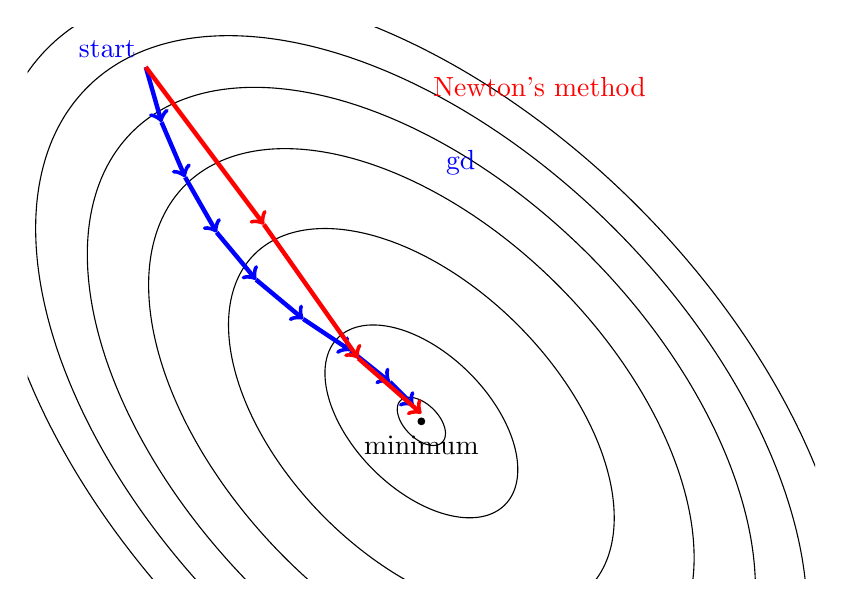
\begin{tikzpicture}[samples=200,smooth]
			\begin{scope}
				\clip(-5,-2) rectangle (5,5);
				\draw[thin] plot[domain=0:360] ({1.5*cos(\x)*sqrt(20/(sin(2*\x)+2))},{1.5*sin(\x)*sqrt(20/(sin(2*\x)+2))});
				\draw[thin] plot[domain=0:360] ({1.5*cos(\x)*sqrt(16/(sin(2*\x)+2))},{1.5*sin(\x)*sqrt(16/(sin(2*\x)+2))});
				\draw[thin] plot[domain=0:360] ({1.5*cos(\x)*sqrt(12/(sin(2*\x)+2))},{1.5*sin(\x)*sqrt(12/(sin(2*\x)+2))});
				\draw[thin] plot[domain=0:360] ({1.5*cos(\x)*sqrt(8/(sin(2*\x)+2))},{1.5*sin(\x)*sqrt(8/(sin(2*\x)+2))});
				\draw[thin] plot[domain=0:360] ({1.5*cos(\x)*sqrt(4/(sin(2*\x)+2))},{1.5*sin(\x)*sqrt(4/(sin(2*\x)+2))});
				\draw[thin] plot[domain=0:360] ({1.5*cos(\x)*sqrt(1/(sin(2*\x)+2))},{1.5*sin(\x)*sqrt(1/(sin(2*\x)+2))});
				\draw[thin] plot[domain=0:360] ({1.5*cos(\x)*sqrt(0.0625/(sin(2*\x)+2))},{1.5*sin(\x)*sqrt(0.0625/(sin(2*\x)+2))});
				% Gradient Descent path
				\draw[->,blue,ultra thick] (-3.5,4.5) -- (-3.3,3.8);
				\draw[->,blue,ultra thick] (-3.3,3.8) -- (-3,3.1);
				\draw[->,blue,ultra thick] (-3,3.1) -- (-2.6,2.4);
				\draw[->,blue,ultra thick] (-2.6,2.4) -- (-2.1,1.8);
				\draw[->,blue,ultra thick] (-2.1,1.8) -- (-1.5,1.3);
				\draw[->,blue,ultra thick] (-1.5,1.3) -- (-0.9,0.9);
				\draw[->,blue,ultra thick] (-0.9,0.9) -- (-0.4,0.5);
				\draw[->,blue,ultra thick] (-0.4,0.5) -- (-0.1,0.2);
				\node[blue,above left] at (-3.5,4.5) {start};
				\node[blue,above] at (0.5,3) {\gls{gd}};
				% Newton's Method path 
				\draw[->,red,ultra thick] (-3.5,4.5) -- (-2,2.5);
				\draw[->,red,ultra thick] (-2,2.5) -- (-0.8,0.8);
				\draw[->,red,ultra thick] (-0.8,0.8) -- (0,0.1);
				\node[red,above] at (1.5,4) {Newton's method};
				\node at (0,0) [circle,fill,inner sep=1pt,label=below:\gls{minimum}] {};
			\end{scope}
		\end{tikzpicture}
		\caption{Comparison of \gls{gd} (blue) and Newton's method (red) paths toward the \gls{minimum} of a 
			\gls{lossfunc}. \label{fig_newtonmethod_dict}}
		\end{figure}
		See also: \gls{optmethod}, \gls{gradient}, \gls{hessian}, \gls{gd}. },
  	first={newtonmethod},
 	type=math,
  	text={newtonmethod} 
}

\newglossaryentry{hilbertspace}
{name={Hilbert space},
	description={A\index{Hilbert space} Hilbert space $\hilbertspace$ is a complete 
    		\gls{innerproduct} space. Thus, $\hilbertspace$ is a \gls{vectorspace} 
		equipped with an \gls{innerproduct} $\innerprod{\cdot}{\cdot}$. The \gls{innerproduct} 
		induces a \gls{norm} $\normgeneric{\cdot}{2}$ via $\normgeneric{\weights}{2} = \sqrt{\innerprod{\weights}{\weights}}$. 
  		Furthermore, $\hilbertspace$ is complete in the sense that every 
 		\gls{cauchysequence} $\big( \weights^{(\sampleidx)} \big)_{\sampleidx \in \mathbb{N}}$ 
		in $\hilbertspace$ converges to a limit $\lim_{\sampleidx\rightarrow \infty} \weights^{(\sampleidx)}$ 
		that is also contained in $\hilbertspace$. 
		\begin{figure}[H]
			\centering
			\begin{tikzpicture}[scale=3]
			% axes (light)
			%\draw[very thin, gray!30] (-1.2,0) -- (1.2,0);
			%\draw[very thin, gray!30] (0,-1.2) -- (0,1.2);
			% unit circle for visual context
			\draw[gray!40] (0,0) circle (1);
			% parameters
			\def\ang{35} % angle of v (degrees)
			% vectors
			\draw[->,thick] (0,0) -- (1,0) node[below right] {$\vu$};
			\draw[->,thick] (0,0) -- ({cos(\ang)},{sin(\ang)}) node[above] {$\vv$};
			% projection of v onto u
			\coordinate (P) at ({cos(\ang)},0);
			\draw[dashed] ({cos(\ang)},{sin(\ang)}) -- (P);
			\draw[->,thick] (0,0) -- (P) node[pos=0.5,below] {$\innerprod{\vv}{\vu} \vu$};
			% right-angle marker at foot of perpendicular
			\draw ($(P)+(0,0.06)$) -- (P) -- ($(P)+(-0.06,0)$);
			% angle arc and label
			%\draw (0.35,0) arc (0:\ang:0.35);
			%\node at ({0.48*cos(\ang/2)},{0.48*sin(\ang/2)}) {$\theta$};	
			% norm labels (unit vectors)
			%\node[below] at (1,0) {$\|\mathbf u\|=1$};
			\node[right] at ({cos(-\ang)},{sin(-\ang)}) {$\sphere{\nrfeatures} = \{ \weights \in \mathbb{R}^{\nrfeatures}: \innerprod{\weights}{\weights}=1\}$};
			% inner product hint
			%\node[below] at (P) {$\langle \mathbf u,\mathbf v\rangle=\cos\theta$};
			\end{tikzpicture}
		\caption{For two unit-\gls{norm} \glspl{vector} $\vu, \vv \in \sphere{\nrfeatures} \subseteq \mathbb{R}^{\nrfeatures}$ 
			the \gls{innerproduct} $\innerprod{\vu}{\vv}$ is the expansion coefficient for the \gls{projection} 
			of $\vv$ onto the \gls{subspace} $\{ c \vu: c \in \reals \}$ spanned by $\vu$. 
			The absolute value $|\innerprod{\vu}{\vv}|$ measures the \gls{norm} of this \gls{projection}.\label{fig_hilbertspace_dict}}
		\end{figure}
		One important example of a Hilbert space 
 		is the \gls{euclidspace} $\mathbb{R}^{\nrfeatures}$ with the 
 		\gls{innerproduct} $\innerprod{\weights}{\weights'} = \weights^{\top} \weights'$. 
		\\
   		See also: \gls{vectorspace}.},
   	type=math, 
 	first={Hilbert space}, 
    	text={Hilbert space},
   	plural={Hilbert spaces},
   	firstplural={Hilbert spaces}
}

\newglossaryentry{cauchysequence}
{name={Cauchy sequence},
	description={A\index{Cauchy sequence} Cauchy \gls{sequence} is a \gls{sequence}
		$\big( \featurevec^{(\sampleidx)}\big)_{\sampleidx \in \mathbb{N}}$ 
		in a \gls{metricspace} $\pair{\featurespace}{\metric{\cdot}{\cdot}}$ such 
		that the elements $\featurevec^{(\sampleidx)}\in \featurespace$ 
		become arbitrarily close to each other eventually. 
		In other words \cite[Def. 3.8]{RudinBookPrinciplesMatheAnalysis}, 
		\[
		\forall \epsilon > 0, \exists N \in \mathbb{N} \text{ such that } 
		\forall \sampleidx, \sampleidx' \geq N, \ \metric{\featurevec^{(\sampleidx)}}{\featurevec^{(\sampleidx')}} < \epsilon.
		\] 
		Fig.\ \ref{fig:fpit_cauchy_sqrt2_dict} shows a Cauchy \gls{sequence} in the \gls{metricspace} $\pair{\mathbb{Q}}{|\cdot|}$ of 
		rational numbers.  
		\begin{figure}[H]
			\centering
		  	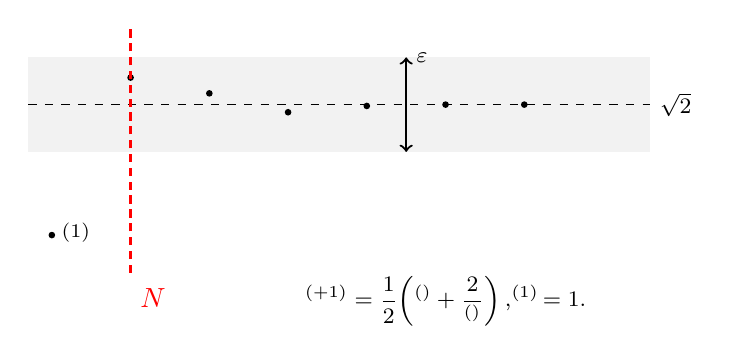
\begin{tikzpicture}[x=1cm,y=4cm]
			% Parameters
			\def\srtwo{1.4142}
			\def\eps{0.15}
			\def\nmax{7}
			% Axes
			% \draw[->] (-0.3,0) -- (\nmax+0.6,0) node[right] {$\sampleidx$};
			% \draw[->] (-0.3,0.9) -- (-0.3,1.46) node[above] {$x^{(\sampleidx)}$};
			% epsilon band around sqrt(2)
			\fill[gray!30, opacity=0.35]
			(-0.3,{\srtwo-\eps}) rectangle (\nmax+0.6,{\srtwo+\eps});
			%	\draw[dotted] (-0.3,{\srtwo+\eps}) -- (\nmax+0.6,{\srtwo+\eps})
			%	node[right] {\footnotesize{$\sqrt{2}+\varepsilon$}};
			%	\draw[dotted] (-0.3,{\srtwo-\eps}) -- (\nmax+0.6,{\srtwo-\eps})
			%	node[right] {\footnotesize{$\sqrt{2}-\varepsilon$}};
			% Double arrow showing epsilon band width
			\draw[<->, thick] (4.5,{\srtwo-\eps}) -- (4.5,{\srtwo+\eps})
			node[above, right] {\footnotesize{$\varepsilon$}};
			% Limit line at sqrt(2)
			\draw[dashed] (-0.3,\srtwo) -- (\nmax+0.6,\srtwo)
			node[right] {\footnotesize{$\sqrt{2}$}};
			% Sequence via fixed-point iteration: x_{n+1} = 0.5(x_n + 2/x_n), x_0 = 1
			% Replace the foreach loop by:
			\fill (0,1.0000) circle (1.2pt) node [right] {$\feature^{(1)}$};
			\fill (1,1.5000) circle (1.2pt);
			% \fill (2,1.4167) circle (1.2pt);
			% \fill (3,1.4142) circle (1.2pt);
			% \fill (4,1.41421) circle (1.2pt);
			% \fill (5,1.4142136) circle (1.2pt);
			% \fill (6,1.41421356) circle (1.2pt);
                %%% minor adaption of figure - by "naked eye" the final values of the sequence are hard to distinguish from 
                %%% the limit \sqrt{2}. In this way, it is illustrated more clearly that this doesn't need to be the case for convergence.
                %%% furthermore, it also avoids the illusion of monotonicity, by including jumps above and below the limit.
                \fill (2,1.45) circle (1.2pt);
			\fill (3,1.39) circle (1.2pt);
			\fill (4,1.41) circle (1.2pt);
			\fill (5,1.4142136) circle (1.2pt);
			\fill (6,1.41421356) circle (1.2pt);
			% Choose an N (first index within eps-band) -- here N=3 works for eps=0.005
			\def\N{1}
			\draw[densely dashed, thick, red] (\N,0.88) -- (\N,1.655);
			\node[right, red] at (\N,0.8) {$N$};
			% Formula box (fixed-point iteration)
			\node[align=right, anchor=north, font=\small]
			at (5,0.9)
			{\footnotesize{$\displaystyle \feature^{(\sampleidx+1)}=\frac{1}{2}\!\left(\feature^{(\sampleidx)}+\frac{2}{\feature^{(\sampleidx)}}\right), \feature^{(1)}=1.$}};
			% Optional: annotate a few rational iterates
			%	\node[font=\scriptsize, anchor=west] at (0,1.5-0.06) {$x^{(1)}=\tfrac{3}{2}$};
			%	\node[font=\scriptsize, anchor=west] at (1,1.5-0.12) {$x^{(2)}=\tfrac{17}{12}$};
			%	\node[font=\scriptsize, anchor=west] at (2,1.5-0.145) {$x^{(3)}=\tfrac{577}{408}$};
			\end{tikzpicture}
		\caption{A Cauchy \gls{sequence} $\big(\feature^{(\sampleidx)}\big)_{\sampleidx\in\mathbb{N}}$ 
			in the \gls{metricspace} $\pair{\mathbb{Q}}{|\cdot|}$. 
			This \gls{sequence} is generated by a \gls{fixedpointiter} used to approximate 
			$\sqrt{2}$. For all $\sampleidx \ge N$, the \gls{sequence} elements lie within a band of width $\varepsilon$. 
			Note that the \gls{sequence} does not converge in $\mathbb{Q}$, 
			since $\sqrt{2} \notin \mathbb{Q}$ \cite[Example 1.1]{RudinBookPrinciplesMatheAnalysis}.\label{fig:fpit_cauchy_sqrt2_dict}}
		\end{figure}
		See also: \gls{sequence}, \gls{metricspace}, \gls{convergence}. }, 
	type=math,
	first={Cauchy sequence},
	text={Cauchy sequence},
	plural={Cauchy sequences},
	firstplural={Cauchy sequences}
}

\newglossaryentry{nonexpansiveop}
{name={non-expansive operator},
 	description={An\index{non-expansive operator} \gls{operator} 
		$\fixedpointop: \hilbertspace \rightarrow \hilbertspace$ defined on a 
		\gls{hilbertspace} $\hilbertspace$ is called non-expansive if it does 
		not increase distances. 
		In other words,  
 		\begin{equation} 
 			\nonumber
 			\normgeneric{ \fixedpointop \weights - \fixedpointop \weights'}{2} 
			\leq 	\normgeneric{\weights - \weights'}{2} \mbox{ for any } \weights, \weights' \in \hilbertspace. 
 		\end{equation} 
		Non-expansiveness is typically not sufficient to guarantee \gls{convergence} 
		of a \gls{fixedpointiter} that uses $\fixedpointop$ (see Fig.\ \ref{fig_nonexpansiveop_dict}).
		\begin{figure}[H]
			\centering
			\begin{tikzpicture}[thick,font=\small]
			\node[circle,fill=black,inner sep=1.6pt,label=below:{$\weights^\star$}] at (0,0) {};
			\draw[dashed] (0,0) circle[radius=2.7];
			\node[circle,fill=black,inner sep=1.6pt,label=right:{$\weights$}] at (2.3,1.4) {};
			\node[circle,fill=black,inner sep=1.6pt,label=below:{$\fixedpointop \weights$}] at (1.27,0.77) {};
			\node[circle,fill=black,inner sep=1.6pt,label=above:{$\fixedpointop' \weights$}] at (-0.23,2.68) {};
			\node[circle,fill=black,inner sep=1.6pt,label=below:{$\fixedpointop''\weights$}] at (1.03,2.04) {};
			\end{tikzpicture}
		\caption{The result of applying a \gls{contractop} $\fixedpointop$, a \gls{nonexpansiveop} 
		         $\fixedpointop'$, and a \gls{firmlynonexpansiveop} $\fixedpointop''$. These 
			\glspl{operator} have the common \gls{fixedpoint} $\weights^\star$. \label{fig_nonexpansiveop_dict}}
       		\end{figure}
 		See also: \gls{fixedpointiter}, \gls{contractop}.},
 	type=math, 
	first={non-expansive operator},
 	plural={non-expansive operators},
	firstplural={non-expansive operators},
 	text={non-expansive operator}
}

\newglossaryentry{firmlynonexpansiveop}
{name={firmly non-expansive operator},
 	description={An\index{firmly non-expansive operator} \gls{operator} 
		$\fixedpointop: \hilbertspace \rightarrow \hilbertspace$ defined on a 
		\gls{hilbertspace} $\hilbertspace$ is called firmly non-expansive if it satisfies 
 		\begin{equation} 
 			\nonumber
 			\normgeneric{ \fixedpointop \weights - \fixedpointop \weights'}{2}^2  
			\leq 	\innerprod{ \weights - \weights'}{ \fixedpointop \weights - \fixedpointop \weights'} 
			\mbox{ for any } \weights, \weights' \in \hilbertspace. 
 		\end{equation}
		Any firmly \gls{nonexpansiveop} is necessarily also a \gls{nonexpansiveop} \cite{BausckeCombette}. 
		Every \gls{fixedpointiter} that uses a firmly \gls{nonexpansiveop} converges 
		to a fixed point of the \gls{operator} \cite{BausckeCombette}.
		\\ 
 		See also: \gls{fixedpointiter}, \gls{contractop}.},
 	type=math, 
	first={firmly non-expansive operator},
 	plural={firmly non-expansive operators},
	firstplural={firmly non-expansive operators},
 	text={firmly non-expansive operator}
}

\newglossaryentry{fixedpointiter}
{name={fixed-point iteration},
	description={A\index{fixed-point iteration} fixed-point \gls{iteration} is an iterative method 
	    for solving a \gls{fixedpointeq}, which in an \gls{ml} context often arises from an \gls{optproblem}. 
            It constructs a \gls{sequence} $\weights^{(0)}, \,\weights^{(1)}, \,\ldots$ by 
		repeatedly applying an \gls{operator} $\fixedpointop$, i.e., 
		\begin{equation} 
		 	\label{equ_def_fixed_point_dict} 
		 	\weights^{(\iteridx+1)} = \fixedpointop \weights^{(\iteridx)} \mbox{, for } \iteridx=0, \,1, \,\ldots.
		\end{equation} 
		The \gls{operator} $\fixedpointop$ is chosen such that any of its \glspl{fixedpoint} is a solution 
		$\widehat{\weights}$ to the given \gls{optproblem}. For example, given a \gls{differentiable} and 
		\gls{convex} \gls{function} $f(\weights)$, the fixed points of the \gls{operator} $\fixedpointop: \weights \mapsto \weights - \nabla f(\weights)$ 
		coincide with the minimizers of $f(\weights)$. In general, for a given \gls{optproblem} 
		with solution $\widehat{\weights}$, there are many different \glspl{operator} 
		$\fixedpointop$ whose fixed points are $\widehat{\weights}$. Clearly, we should use an 
		\gls{operator} $\fixedpointop$ in \eqref{equ_def_fixed_point_dict} that reduces the 
		distance to a solution such that
		\begin{equation} 
			\nonumber
			\underbrace{\normgeneric{ \weights^{(\iteridx+1)} - \widehat{\weights}}{2}}_{\stackrel{\eqref{equ_def_fixed_point_dict}}{=} \normgeneric{ \fixedpointop \weights^{(\iteridx)} - \fixedpointop\widehat{\weights}}{2}}  \leq 	\normgeneric{ \weights^{(\iteridx)} - \widehat{\weights}}{2}. 
		\end{equation}
		Thus, we require $\fixedpointop$ to be at least a \gls{nonexpansiveop}, i.e., the \gls{iteration} \eqref{equ_def_fixed_point_dict} 
		should not result in worse \glspl{modelparam} that have a larger distance to a solution $\widehat{\weights}$. 
		Furthermore, each \gls{iteration} \eqref{equ_def_fixed_point_dict} should also make some progress, i.e., 
		reduce the distance to a solution $\widehat{\weights}$. This requirement can be made precise using 
		the notion of a \gls{contractop} \cite{Bauschke:2017}, \cite{fixedpoinIsta}. 
		The \gls{operator} $\fixedpointop$ is a \gls{contractop} if, for some $\contractfac \in [0,1)$,
		\begin{equation} 
			\nonumber
			\normgeneric{ \fixedpointop \weights\!-\!\fixedpointop \weights'}{2}  \leq  \contractfac	\normgeneric{\weights\!-\!\weights'}{2} \mbox{ holds for any } \weights,\weights'.
		\end{equation}
		For a \gls{contractop} $\fixedpointop$, the fixed-point \gls{iteration} \eqref{equ_def_fixed_point_dict} generates 
		a \gls{sequence} $\weights^{(\iteridx)}$ that converges quite rapidly. In particular \cite[Th. 9.23]{RudinBookPrinciplesMatheAnalysis}, 
		\begin{equation} 
			\nonumber
			\normgeneric{ \weights^{(\iteridx)} - \widehat{\weights}}{2} \leq \contractfac^{\iteridx} 	\normgeneric{ \weights^{(0)} - \widehat{\weights}}{2}. 
		\end{equation} 
		Here, $\normgeneric{ \weights^{(0)} - \widehat{\weights}}{2}$ is the distance between 
		the initialization $\weights^{(0)}$ and the solution $\widehat{\weights}$. 
		It turns out that a fixed-point \gls{iteration} \eqref{equ_def_fixed_point_dict} with a 
		\gls{firmlynonexpansiveop} $\fixedpointop$ is guaranteed to converge to a 
		\gls{fixedpoint} of $\fixedpointop$ \cite[Corollary 5.16]{Bauschke:2017}. 
		Fig. \ref{fig_examples_nonexp_dict} depicts examples of a \gls{nonexpansiveop}, 
		a \gls{firmlynonexpansiveop}, and a \gls{contractop}. All of these \glspl{operator} are 
		defined on the 1-D space $\mathbb{R}$. Another example of a \gls{firmlynonexpansiveop} 
		is the \gls{proxop} of a \gls{convex} \gls{function} \cite{ProximalMethods}, \cite{Bauschke:2017}. 
		\definecolor{darkgreen}{rgb}{0.0, 0.5, 0.0}
		\begin{figure}[H]
			\begin{center} 
				\begin{tikzpicture}[scale=1.5]
					% Axes
					\draw[line width=1pt, ->] (-2,0) -- (2,0) node[right] {$\weight^{(\iteridx)}$};
					\draw[line width=1pt, ->] (0,-2) -- (0,2) node[above] {$\weight^{(\iteridx+1)}$};
					% Labels
					\node at (2.1,2.2) {$\fixedpointop^{(3)}$};
					\node at (1.9,-1.5) {$\fixedpointop^{(1)}$};
					\node at (1.5,1.2) {$\fixedpointop^{(2)}$};
					% Dashed lines at x=1 and y=1
					\draw[dashed] (1,-2) -- (1,2); % Vertical line at x=1
					\draw[dashed] (-2,1) -- (2,1); % Horizontal line at y=1
					\draw[dashed] (-2,-1) -- (2,-1); % Horizontal line at y=1
					\draw[dashed] (-1,-2) -- (-1,2); % Vertical line at x=1
					\node[above,xshift=4pt,yshift=-1pt] at (1,0) {$1$};
					\node[above,xshift=8pt,yshift=-1pt] at (0,-1) {$-1$};
					% First curve: y = 1/2 x + 1
					\draw[line width=2,domain=-2:2,smooth,blue] plot(\x,{0.5*\x + 1});
					% Second curve: y = -x
					\draw[line width=2,domain=-2:2,smooth,red] plot(\x,{-\x});
					% Third curve: y = x / |x| * min(|x|, 1)
					\draw[line width=2, domain=-2:-1,smooth,darkgreen] plot(\x,{-1});
					\draw[line width=2,domain=-1:1,smooth,darkgreen] plot(\x,{\x});
					\draw[line width=2,domain=1:2,smooth,darkgreen] plot(\x,{1});
				\end{tikzpicture}
			\end{center} 
			\caption{Example of a \gls{nonexpansiveop} $\fixedpointop^{(1)}$, a \gls{firmlynonexpansiveop} 
				$\fixedpointop^{(2)}$, and a \gls{contractop} $\fixedpointop^{(3)}$. \label{fig_examples_nonexp_dict}}
		\end{figure} 
		See also: \gls{contractop}, \gls{proxop}, \gls{bellmanoperator}, \gls{policyevaluation}, \gls{valueiteration}.},
	first={fixed-point iteration},
	text={fixed-point iteration},
	type=math, 
	firstplural={fixed-point iterations}, 
	plural={fixed-point iterations}
}

\newglossaryentry{graphoffunction}
{name={graph of a function},
 description={Given\index{graph of a function} a \gls{function} $f\!:\!\featurespace \to \labelspace$
                with \gls{domain} $\featurespace$ and \gls{co-domain} $\labelspace$, 
			  the graph of $f$ is the subset of $\featurespace \times \labelspace$ 
			  defined as
				\[
				  \{ (\featurevec,f(\featurevec)) : \featurevec \in \featurespace \,\}.
				\]
				The graph of a \gls{function} provides a geometric representation 
				that is widely used in analysis, topology, and optimization \cite{MunkresTopology2000,RockafellarBook}.
                    \\ 
                    See also: \gls{epigraph}.}, 
	first={graph},
	text={graph},
	type=math, 
	firstplural={graphs},
	plural={graphs}
}

\newglossaryentry{epigraph}
{name={epigraph},
	description={The epigraph\index{epigraph} of a real-valued \gls{function} 
		$f : \mathbb{R}^n \to \mathbb{R} \cup \{+\infty\}$ 
  		is the set of points lying on or above its \gls{graphoffunction} 
		(see Fig. \ref{fig_epigraph_dict}), i.e., 
		\[
		\operatorname{epi}(f) = \left\{ (\mathbf{x}, t) \in \mathbb{R}^n \times \mathbb{R} \,\middle|\, f(\mathbf{x}) \leq t \right\}.
		\]
		A \gls{function} is \gls{convex} if and only if its epigraph is a 
		\gls{convex} set \cite{BoydConvexBook}, \cite{BertCvxAnalOpt}.
		\begin{figure}[H]
			\centering
			\begin{tikzpicture}[scale=1.0]
				\begin{axis}[
					axis lines = middle,
					xlabel = $x$,
					ylabel = {},
					xmin=-2, xmax=2,
					ymin=0, ymax=4.5,
					samples=100,
					domain=-1.5:1.5,
					thick,
					width=8cm,
					height=6cm,
					grid=none,
					axis on top,
					]
					% Function
					\addplot [blue, thick, domain=-1.5:1.5] {x^2} node [pos=0.85, anchor=south west, xshift=5pt] {$f(\weights)$};
					% Epigraph shading
					\addplot [
					name path=f,
					draw=none,
					ytick=\empty,
					domain=-1.5:1.5,
					] {x^2};
					\path[name path=top] (axis cs:-1.5,4) -- (axis cs:1.5,4);
					\addplot [
					blue!20,
					opacity=0.6,
					draw=none,
					] fill between [
					of=f and top,
					soft clip={domain=-1.5:1.5},
					];
					    \node[font=\small] at (axis cs:-1.0,2.3) {$\operatorname{epi}(f)$};
				%	\node[align=center, fill=white, draw=black, rounded corners, font=\small] at (axis cs:0.5,3.5) {Epigraph\\$\{(x,t) \mid f(x) \le t\}$};
				\end{axis}
			\end{tikzpicture}
		\caption{Epigraph of the \gls{function} $f(x) = x^2$ (i.e., the shaded area). \label{fig_epigraph_dict}}
		\end{figure}
		See also: \gls{function}, \gls{convex}.},
	first={epigraph},
	text={epigraph},
	type=math,
	firstplural={epigraphs},
	plural={epigraphs}
}

\newglossaryentry{nullspace}
{name={nullspace},
	description={The nullspace\index{nullspace} of a \gls{matrix} $\mA \in \mathbb{R}^{\nrfeatures' \times \nrfeatures}$, 
		denoted by $\nullspace{\mA}$, is the set of all \glspl{vector} $\mathbf{n} \in \mathbb{R}^\nrfeatures$ 
    		such that $$\mA \mathbf{n} = \mathbf{0}.$$ 
		Consider a \gls{featlearn} method that uses the \gls{matrix} $\mA$ to transform 
		a \gls{featurevec} $\mathbf{x} \in \mathbb{R}^{\nrfeatures}$ of a \gls{datapoint} 
		into a new \gls{featurevec} $\vz = \mA \mathbf{x} \in \mathbb{R}^{\nrfeatures'}$. 
		The nullspace $\nullspace{\mA}$ characterizes all directions in the original 
    		\gls{featurespace} $\mathbb{R}^{\nrfeatures}$ along which the transformation 
		$\mA \mathbf{x}$ remains unchanged. In other words, adding any \gls{vector} from 
		the nullspace to a \gls{featurevec} $\featurevec$ does not affect the transformed 
		representation $\vz$. This property can be exploited to enforce invariances in the 
		\glspl{prediction} (computed from $\mA \mathbf{x}$). Fig.\ \ref{fig:nullspace-rotation-dict} 
		illustrates one such invariance. It shows rotated versions of two handwritten digits, 
		which approximately lie along 1-D curves in the original \gls{featurespace}. 
		These curves are aligned with a direction \gls{vector} $\mathbf{n} \in \mathbb{R}^{\nrfeatures}$. 
    		To ensure that the trained \gls{model} is invariant to such rotations, we can 
		choose the transformation \gls{matrix} $\mA$ such that $\mathbf{n} \in \nullspace{\mA}$. 
		This ensures that $\mA \mathbf{x}$, and hence the resulting \gls{prediction}, 
		is approximately insensitive to rotations of the input image.
		\begin{figure}[H]
      			\centering
      			\includegraphics[width=0.6\textwidth]{assets/pythonsnacks/nullspace/nullspace_0_1.png}
	  		\caption{
			Rotated handwritings of two different digits. The rotations are approximately 
			aligned along straight lines parallel to the \gls{vector} $\mathbf{n}$. For a 
			binary \gls{classifier} distinguishing between these digits, a natural choice is 
			a linear \gls{featuremap} $\featurevec \mapsto \mathbf{A}\featurevec$ with a 
			\gls{matrix} $\mA$ whose nullspace contains $\mathbf{n}$, i.e., $\mathbf{n} \in \mathrm{null}(\mA)$.
                \label{fig:nullspace-rotation-dict}}	
	       	\end{figure}
		See also: \gls{matrix}, \gls{featuremap}, \gls{featlearn}. \\ 
		Python demo: \href{https://github.com/AaltoDictionaryofML/AaltoDictionaryofML.github.io/blob/main/assets/pythonsnacks/nullspace/nullspace.py}{click me}},
 	first={nullspace},
 	firstplural={nullspaces},
	type=math,
 	plural={nullspaces},
 	text={nullspace}
}

\newglossaryentry{fixedpoint}
% For most ML applications it is sufficient of course to consider Hilbert spaces, mostly just \R^d, of course. 
% Still, other % entries in the dictionary are much more general, e.g. Banach's fixed point theorem is formulated 
% in a general setting.
{name={fixed point},
	description={Consider some \gls{operator} $\fixedpointop: \hilbertspace \rightarrow \hilbertspace$ 
		defined on a \gls{hilbertspace} $\hilbertspace$. A 
		\gls{vector} $\widehat{\weights} \in \hilbertspace$ 
		is called a fixed point\index{fixed point} of the \gls{operator} $\fixedpointop$ 
		if it satisfies 
		\[
			\fixedpointop \widehat{\weights} = \widehat{\weights}.
		\]
		In other words, applying the \gls{operator} $\fixedpointop$ to its fixed 
		point $\widehat{\weights}$ returns the same \gls{vector} $\widehat{\weights}$. 
		Finding a fixed point of a suitable \gls{operator} $\fixedpointop$ is a common 
		approach to solving various \glspl{optproblem} (e.g., an instance of \gls{erm}). 
		A popular method for computing approximations of a fixed point is the \gls{fixedpointiter}.
		\\
		See also: \gls{fixedpointiter}.},
	first={fixed point},
	text={fixed point},
	type=math, 
	firstplural={fixed points}, 
	plural={fixed points}
}

\newglossaryentry{fixedpointeq}
{name={fixed-point equation},
  description={A fixed-point equation\index{fixed-point equation} is an equation of the form
				\[\weights = \fixedpointop(\weights),
				\]
				where $\fixedpointop:\hilbertspace \to \hilbertspace$ is an \gls{operator} defined 
				on a \gls{hilbertspace} $\hilbertspace$.  
				Solving a fixed-point equation amounts to finding the \glspl{fixedpoint} of 
				$\fixedpointop$. Many \glsps{optproblem}, including instances of \gls{erm}, 
				can be cast in this form. For example, minimizing a \gls{smooth} \gls{convex} 
				\gls{function} $f$ is equivalent to solving the fixed-point equation 
				$$\weights = \fixedpointop \weights \mbox{ with }  
				\fixedpointop: \weights \mapsto \weights - \eta \nabla f(\weights).$$
				Here, $\lrate>0$ can be choosen freely. The above fixed-point 
				equation is nothing but the \gls{zerogradientcondition} for the 
				minimizer of $f$ \cite{BoydConvexBook}. Similarly, one can reformulate the
				 optimality conditions (KKT conditions) of \glspl{optproblem} with constraints as a 
				 fixed-point equation \cite{pock_chambolle_2016,BoydConvexBook}}, 
	type=math, 
	first={fixed-point equation},
 	text={fixed-point equation}, 
	plural={fixed-point equations}, 
	firstplural={fixed-point equations}
}

\newglossaryentry{diagonalizable}
{name={diagonalizable},
	description={A square \gls{matrix} $\mA \in \mathbb{C}^{\nrfeatures \times \nrfeatures}$ 
		is called diagonalizable\index{diagonalizable} if it is similar  
 		to a diagonal \gls{matrix} \cite{HornMatAnalysis}, \cite{Axler2025}. 
 		Formally, $\mA$ is diagonalizable if there exists an invertible \gls{matrix} 
		$\mP \in \mathbb{C}^{\nrfeatures \times \nrfeatures}$ such that 
  		\[
  			\mA = \mP \mD \mP^{-1},
  		\]
		where $\mD \in \mathbb{C}^{\nrfeatures \times \nrfeatures}$ is a 
 		diagonal \gls{matrix} whose main diagonal entries are the \glspl{eigenvalue} 
 		of $\mA$. A \gls{matrix} $\mA \in \mathbb{R}^{\nrfeatures \times \nrfeatures}$ 
 		is diagonalizable if and only if it has $\nrfeatures$ linearly independent 
 		\glspl{eigenvector} \cite{HornMatAnalysis}. 
 		\\	
 		See also: \gls{matrix}, \gls{eigenvalue}, \gls{evd}.},
 	first={diagonalizable},
 	type=math,
 	text={diagonalizable}
}

\newglossaryentry{schurdecomp}
{name={Schur decomposition},
	description={Every square \gls{matrix} $\mA \in \mathbb{C}^{\nrfeatures \times \nrfeatures}$ 
		admits a Schur decomposition\index{Schur decomposition} \cite[Th. 7.1.3]{GolubVanLoanBook}
		\[
		\mA = \mU \mT \mU^{H}. 
		\]
		Here, $\mU \in \mathbb{C}^{\nrfeatures \times \nrfeatures}$ is a \gls{unitary} 
		(i.e., $\mU^{H}\mU = \mI$) and $\mT$ is upper triangular 
		with the \glspl{eigenvalue} of $\mA$ on its diagonal.
		Carefully note that the Schur decomposition exists also 
		for a \gls{matrix} $\mA$ that is not \gls{diagonalizable}.
		The identity
		\[
			\big(\mU^{(1)}\big)^{H} \mA \mU^{(1)}
			=
			\begin{pmatrix}
			\big(\vx^{(1)}\big)^{H} \\
			\big(\mX^{(2)}\big)^{H}
			\end{pmatrix}
			\mA
			\begin{pmatrix}
			\vx^{(1)} & \mX^{(2)}
			\end{pmatrix}
			=
			\begin{pmatrix}
			\eigval{1} & \vb^{H} \\
			0 & \mA^{(1)}
			\end{pmatrix}
		\]
		represents the first step in the construction of the Schur decomposition.
		Every \gls{matrix} $\mA \in \mathbb{C}^{n\times n}$ has at least one 
		\gls{eigenvalue} $\eigval{1}$ with a unit-\gls{norm} \gls{eigenvector} 
		$\vx^{(1)}$, $\mA \vx^{(1)} = \eigval{1} \vx^{(1)}$. This 
		\gls{eigenvector} allows us to decompose $\mA$ as shown above. Here, 
		we extend $\vx^{(1)}$ to an orthonormal basis
		$\mQ^{(1)} = \big( \vx^{(1)} \,\big|\, \mX^{(2)} \big)$
		and use $\vb^{H} := \big(\vx^{(1)}\big)^{H} \mA \mX^{(2)}$ and 
		$\mA^{(1)} := \big(\mX^{(2)}\big)^{H} \mA \mX^{(2)}$.
		Applying the same construction recursively to $\mA^{(1)}$ yields the 
		Schur decomposition.
		\\
 		See also: \gls{matrix}, \gls{eigenvalue}, \gls{evd}.},
	first={Schur decomposition},
	type=math,
	text={Schur decomposition}
}

\newglossaryentry{unitary}
{name={unitary matrix},
	description={A square \gls{matrix} $\mU \in \mathbb{C}^{\nrfeatures \times \nrfeatures}$ 
		is called unitary\index{unitary matrix} if its \gls{conjugatetranspose} 
		(or \gls{hermitian} \gls{transpose}) $\mU^{H}$ is also its \gls{inverse}, i.e., if 
 		\[
 			\mU^{H} \mU = \mU \mU^{H} = \mI.
 		\]
 		Equivalently, the columns (and rows) of a unitary \gls{matrix} form an 
		orthonormal \gls{basis} of $\mathbb{C}^{\nrfeatures}$ with respect to the standard 
		\gls{innerproduct} \cite{HornMatAnalysis}, \cite{Axler2025}. 
 		\\
 		See also: \gls{matrix}.},
 	first={unitary matrix},
 	type=math,
 	text={unitary matrix}
}

\newglossaryentry{innerproduct}
{name={inner product},
	description={Consider a \gls{vectorspace} $\featurespace$ over the 
		field $\mathbb{F}$, where $\mathbb{F}$ is either the field of 
		real numbers $\mathbb{R}$ or the field of complex numbers $\mathbb{C}$. 
		An inner product\index{inner product} in $\featurespace$ is 
		a \gls{function} 
 		\[
 			\innerprod{\cdot}{\cdot}: \featurespace \times \featurespace \to \mathbb{F}
 		\]
 		that satisfies the following properties for all 
		$\featurevec, \featurevec', \featurevec'' \in \featurespace$ 
		and all scalars $\alpha \in \mathbb{F}$ \cite{Axler2025}:
 		\begin{itemize}
 			\item Conjugate symmetry: $\innerprod{\featurevec}{\featurevec'} = \overline{\innerprod{\featurevec'}{\featurevec}}$;
 			\item Linearity in the first argument: $\innerprod{\alpha \featurevec + \featurevec''}{\featurevec'} = \alpha \innerprod{\featurevec}{\featurevec'} + \innerprod{\featurevec''}{\featurevec'}$;
 			\item Positive-definiteness: $\innerprod{\featurevec}{\featurevec} \geq 0$, with equality if and only if $\featurevec = \mathbf{0}$.
 		\end{itemize}
 		The pair $(\featurespace, \innerprod{\cdot}{\cdot})$ is called an inner product space. 
		Each inner product induces a \gls{norm} via 
		$\norm{\featurevec} \defeq \sqrt{\innerprod{\featurevec}{\featurevec}}$ for all 
		$\featurevec \in \featurespace$, which in turn induces a \gls{metric} via 
		$\metric{\featurevec}{\featurevec'} \defeq \norm{\featurevec - \featurevec'}$
		for all $\featurevec, \featurevec' \in \featurespace$.
 		\\
 		See also: \gls{norm}, \gls{vector}, \gls{hilbertspace}, \gls{metricspace}.},
 	first={inner product},
 	type=math,
 	text={inner product}
}

\newglossaryentry{trace}
{name={trace},
 	description={The\index{trace} trace $\tr{\mA}$ of a square \gls{matrix} 
		$\mA \in \mathbb{R}^{\nrfeatures \times \nrfeatures}$ is the 
		sum of its diagonal entries \cite{StrangLinAlg2016}. 
		Formally, it is the \gls{linearmap} 
		$$\tr{\cdot}: \mathbb{R}^{\nrfeatures \times \nrfeatures} 
		 \rightarrow \mathbb{R}: \mA \mapsto \sum_{\featureidx=1}^{\nrfeatures} A_{\featureidx,\featureidx}.$$     
    	 	It satisfies the cyclic property $\tr{\mA\mB}=\tr{\mB\mA}$, for any \glspl{matrix} 
    	 	$\mA,\mB \in \mathbb{R}^{\nrfeatures \times \nrfeatures}$ \cite[p. 301]{Axler2025}.
		\begin{figure}[H]
			\begin{center}
			\begin{tikzpicture}[font=\small, every node/.style={inner sep=1pt}]
				% Matrix entries, manually placed
				\node (a11) at (0,0)   {$A_{1,1}$};
				\node (a12) at (1,0)   {$A_{1,2}$};
				\node (a13) at (2,0)   {$A_{1,3}$};
				\node (a21) at (0,-1)  {$A_{2,1}$};
				\node (a22) at (1,-1)  {$A_{2,2}$};
				\node (a23) at (2,-1)  {$A_{2,3}$};
				\node (a31) at (0,-2)  {$A_{3,1}$};
				\node (a32) at (1,-2)  {$A_{3,2}$};
				\node (a33) at (2,-2)  {$A_{3,3}$};
				% Very light bounding box (optional)
				\draw[black] (-0.4,0.4) rectangle (2.4,-2.4);
				% Tight ellipse around diagonal entries
				\coordinate (C) at ($(a11)!0.5!(a33)$);
				\draw[thick] (C) ellipse [x radius=2.1cm, y radius=0.35cm,rotate=-45];
			\end{tikzpicture}
			\end{center}
		\caption{The trace $\tr{\mA}$ of a $3 \times 3$ \gls{matrix} $\mA \in \mathbb{R}^{3\times 3}$ is 
			the sum of three main diagonal entries $A_{1,1}, \,A_{2,2}, \,A_{3,3}$.}
		\end{figure}
		Furthermore, if $\mA$ has \glspl{eigenvalue} $\eigval{1},\,\ldots,\,\eigval{\nrfeatures}$ 
		(each repeated according to its algebraic multiplicity), then
		\[
		\tr{\mA} = \sum_{\featureidx=1}^{\nrfeatures} \eigval{\featureidx}.
		\]
		This identity follows from the invariance of the trace under similarity 
		transformations \cite[Ch.~10]{Axler2025}.
		\\
    		See also: \gls{matrix}, \gls{eigenvalue}.},
    first={trace},
    type=math,
    text={trace}
}
 
\newglossaryentry{stddev}
{name={standard deviation},
	description={The\index{standard deviation} standard deviation of a 
               	real-valued \gls{rv} $\feature$ is defined as the square 
		root of its \gls{variance}, i.e., 
		$\sqrt{\expect\big\{ \big( \feature - \expect\{\feature \} \big)^{2} \big\}}$. 
		\\
    		See also: \gls{rv}, \gls{variance}, \gls{expectation}.},
    first={standard deviation},
    type=math,
    text={standard deviation}
}

\newglossaryentry{sequence}
{name={sequence},
	description={A sequence\index{sequence} is an ordered collection 
		of values from a set $\mathcal{A}$. For example, a sequence of 
	   	values from the set $\mathcal{A} = \{ \star, \otimes \}$ could be 
	   	$$ a = \big( \star, \,\otimes, \,\star, \,\star, \,\otimes, \,\ldots \big). $$
	   	Formally, a sequence $a$ is a \gls{function} \cite{RudinBookPrinciplesMatheAnalysis} 
        		\[
            	a: \mathbb{N} \rightarrow \mathcal{A}: \sampleidx \mapsto a_\sampleidx.
        		\]        
		We denote a sequence by $\big( a_{\sampleidx} \big)_{\sampleidx \in \mathbb{N}}$ 
		or $\big( a^{(\sampleidx)} \big)_{\sampleidx \in \mathbb{N}}$. Sometimes we also 
		use the notation $\big\{ a^{(\sampleidx)} \big\}_{\sampleidx \in \mathbb{N}}$. 
        		Note that the same value $a \in \mathcal{A}$ can appear multiple times 
		in the sequence at different positions $\sampleidx$. 		
        		Sequences are fundamental for the study of \gls{ml} methods, 
        		for instance when describing successive iterates  
        		$\{\weights^{(\iteridx)}\}_{\iteridx \in \mathbb{N}}$ of an iterative 
		\gls{algorithm} updating a \gls{parameter} \gls{vector}. 
            We can also use a sequence to represent an infinite \gls{dataset} 
		$$\dataset = \big\{ \pair{\featurevec^{(1)}}{\truelabel^{(1)}},\,\pair{\featurevec^{(2)}}{\truelabel^{(2)}},\,\ldots \big\}.$$ 
		See also: \gls{function}, \gls{convergence}, \gls{cauchysequence}, \gls{dataset}. }, 
	first={sequence},
	text={sequence},
	type=math, 
	firstplural={sequences},
	plural={sequences}
}

\newglossaryentry{convergence}
{name={convergence},
	description={Consider a \gls{sequence}\index{convergence} $\big( a_{\sampleidx} \big)_{\sampleidx \in \mathbb{N}}$ 
		with numeric values $a_{\sampleidx} \in \mathbb{R}$. This \gls{sequence} 
       	 	is said to converge to a value $a^\star$ if the values $a_{\sampleidx}$ become 
		arbitrarily close to $a^\star$ for sufficiently large indices $\sampleidx$. 
        		Mathematically speaking, the \gls{sequence} converges to $a^\star$ if 
		\cite{RudinBook}, \cite{RudinBookPrinciplesMatheAnalysis}
        		\[
           	\forall \epsilon > 0, \; \exists N \in \mathbb{N} : \sampleidx > N \Rightarrow |a_{\sampleidx} - a^\star| < \epsilon.
        		\]
		We denote the convergence of a \gls{sequence} to $a^\star$ 
		by 
		\[
			\lim_{\sampleidx \to \infty} a_{\sampleidx} = a^\star.
		\]
		\begin{figure}[H] 
			\centering
			\begin{tikzpicture}[x=1.2cm, y=2cm, >=stealth]
			% Axes
			\draw[->] (0.5,0) -- (6.5,0) node[right] {$\sampleidx$};
			\draw[->] (0.5,0) -- (0.5,1.6) node[above] {$a_\sampleidx$};
			% Epsilon neighbourhood (ε = 0.1)
  			\def\eps{0.3}
  			\fill[gray!30, opacity=0.4] (0, {1-\eps}) rectangle (6.3, {1+\eps});
  			\draw[dotted] (0,{1+\eps}) -- (6.3,{1+\eps}) node[right] {$1+\varepsilon$};
  			\draw[dotted] (0,{1-\eps}) -- (6.3,{1-\eps}) node[right] {$1-\varepsilon$};
			% Limit line at 1
			\draw[dashed] (0,1) -- (6.3,1) node[right] {$\lim_{\sampleidx \to \infty} a_\sampleidx = 1$};
			% Sequence points (e.g. a_t = 1 - 0.6^t)
			\foreach \t in {1,...,6} {
			\pgfmathsetmacro{\at}{1 - 0.6^(\t)}
			\fill (\t,\at) circle (2pt);
			}
			% Tick marks at t = 1, 2, 3
 		     	\foreach \t in {1,2,3} {
    		    	\draw (\t,0.02) -- (\t,-0.02) node[below] {$\t$};
  		    	}
			% Indicate N (first index within ε-band)
  			\def\N{3}
  			\draw[densely dashed, thick, red] (\N,0) -- (\N,1.7);
  			\node[above] at (\N,1.7) {$N$};
			\end{tikzpicture}
		\caption{A real-valued \gls{sequence} $\big( a_{\sampleidx} \big)_{\sampleidx \in \mathbb{N}}$ 
			converging to the limit $a^\star = 1$.\label{fig:convergence_dict}}
		\end{figure} 
		The concept of convergence of a real-valued \gls{sequence} 
		(where $\mathcal{A}=\mathbb{R}$) extends naturally to a \gls{sequence} 
		in an arbitrary \gls{metricspace} $\mathcal{A}$. Indeed, we just need to 
		replace the absolute difference $|a_{\sampleidx} - a^\star|$ 
		by the \gls{metric} $\metric{a_{\sampleidx}}{a^\star}$. 
		Note that a \gls{sequence} can only converge if it is a 
		\gls{cauchysequence} \cite{RudinBookPrinciplesMatheAnalysis}. 
		However, not every \gls{cauchysequence} is converging unless 
		the underlying \gls{metricspace} is complete.   
		\\ 
		See also: \gls{sequence}, \gls{metricspace}, \gls{cauchysequence}.},
	first={convergence},
	type=math,
	text={convergence}, 
}

\newglossaryentry{johnsonlindenstrausslemma}
{name={Johnson--Lindenstrauss lemma (JL lemma)},
	description={The\index{Johnson--Lindenstrauss lemma (JL lemma)} JL lemma describes conditions for 
  		the existence of a \gls{featuremap} $\featuremapvec: \mathbb{R}^{\nrfeatures} \to \mathbb{R}^{\nrfeatures'}$ 
  		with $\nrfeatures' \ll \nrfeatures$ such that the pairwise \gls{eucliddist} 
  		between \glspl{featurevec} of a finite \gls{dataset} is approximately preserved 
  		\cite{vershynin2018high}, \cite{JMLR:v19:18-264}, \cite{johnson1984extensions}. 
  		Consider a \gls{dataset} $\dataset = \big\{\featurevec^{(1)}, \,\dots, \,\featurevec^{(\samplesize)} \big\}$ 
  		with \glspl{datapoint} characterized by \glspl{featurevec} in $\mathbb{R}^{\nrfeatures}$. 
  		Then, for any $\nrfeatures'$ that satisfies
		\[
	  	\nrfeatures' \ge \frac{4 \ln(\samplesize)}{\varepsilon^2/2 - \varepsilon^3/3} \mbox{ for some } 0 < \varepsilon < 1
		\]  
   		there is a \gls{featuremap} $\featuremapvec$ such that \cite{ProofJLlemma}
  		\begin{equation} 
 			\label{equ_def_approx_norm_JL_lemma_dict}
 			(1\!-\!\varepsilon)\normgeneric{\featurevec^{(\sampleidx)}\!-\!\featurevec^{(\sampleidx')}}{2}  
 			\!\le\!\normgeneric{\featuremapvec\big(\featurevec^{(\sampleidx)}\big)\!-\!\featuremapvec\big(\featurevec^{(\sampleidx')}\big)}{2} 
			\!\le\!(1\!+\!\varepsilon)\normgeneric{\featurevec^{(\sampleidx)}\!-\!\featurevec^{(\sampleidx')}}{2}
 		\end{equation}
		for all $\featurevec^{(\sampleidx)}, \featurevec^{(\sampleidx')} \in \dataset$. 
		\begin{figure}[H]
			\centering
			\begin{tikzpicture}
			% ---------- Original space: R^d ----------
			\begin{scope}
				% Points
				\coordinate (x1) at (0.5,-0.6);   % anchor
				\coordinate (x2) at (2.0,0.9);    % farther from x1 (long)
				\coordinate (x3) at (1.1,0.3);    % closer to x1 (short)
				\foreach \p in {x1,x2,x3} \fill (\p) circle (1.7pt);
				% Labels
				\node[below left]  at (x1) {\small $\featurevec^{(1)}$};
				\node[above right] at (x2) {\small $\featurevec^{(2)}$};
				\node[above left]  at (x3) {\small $\featurevec^{(3)}$};
				\node [anchor=east] at (1.2,2.2) {$\mathbb{R}^{\nrfeatures}$};
			\end{scope}
			% ---------- Mapping arrow ----------
			\begin{scope}[xshift=1cm]
				\draw[->, thick] (2.9,2.2) -- (4.1,2.2)
				node[midway, above] {$\featurevec \mapsto \vz \!\defeq\! \featuremapvec(\featurevec)$};
			\end{scope}
			% ---------- Transformed space: R^{d'} ----------
			\begin{scope}[xshift=2cm]
				% Images of points (preserving relative distances)
				\coordinate (y1) at (4.7,-0.7);   % image of x1
				\coordinate (y2) at (6.1,0.5);    % image of x2 (farther)
				\coordinate (y3) at (5.3,-0.1);   % image of x3 (closer)
				\foreach \p in {y1,y2,y3} \fill (\p) circle (1.7pt);
				\node[below left]  at (y1) {\small $\vz^{(1)}$};
				\node[above right] at (y2) {\small $\vz^{(2)}$};
				\node[above left]  at (y3) {\small $\vz^{(3)}$};
				\node [anchor=west] at (6.0,2.2) {$\mathbb{R}^{\nrfeatures'}$};
			\end{scope}
			\end{tikzpicture}
		\caption{The JL lemma offers precise conditions that guarantee the existence of 
		         a \gls{featuremap} $\featuremapvec: \mathbb{R}^{\nrfeatures} \rightarrow \mathbb{R}^{\nrfeatures'}$ 
		         such that pairwise \glspl{eucliddist} between (the \glspl{featurevec} of) \glspl{datapoint} are 
			approximately preserved. Roughly speaking, 
			$\featuremapvec$ maps neighboring points in the original \gls{featurespace} 
			to neighboring points in the new \gls{featurespace}.}
		\end{figure}
		The \gls{featuremap} $\featuremapvec$ can be obtained from a random \gls{matrix} 
		$\mA \in \mathbb{R}^{\nrfeatures' \times \nrfeatures}$ whose entries are \gls{iid} 
		\glspl{gaussrv} $A_{i,j} \sim \mvnormal{0}{1/\nrfeatures'}$. 
		It can be shown that the \gls{featuremap} $\featurevec \mapsto \underbrace{\mA \featurevec}_{\featuremapvec(\featurevec)}$ 
		satisfies \eqref{equ_def_approx_norm_JL_lemma_dict} with \gls{probability} at least $1\!-\!1/\samplesize$ \cite{ProofJLlemma}. 
		\\
  		See also: \gls{matrix}, \gls{norm}, \gls{vectorspace}, \gls{euclidspace}, \gls{dimred}, \gls{pca}.},	
	first={Johnson--Lindenstrauss lemma (JL lemma)},
	type=math, 
  	text={JL lemma}
}

\newglossaryentry{admm}
{name={alternating direction method of multipliers (ADMM)},
 description={The \index{alternating direction method of multipliers (ADMM)} 
               alternating direction method of multipliers (ADMM) 
  			  is an iterative \gls{optmethod} for solving a structured \glspl{optproblem}. 
			  In particular, ADMM can be used to solve an \gls{optproblem} of the form 
			  \[
			  \min_{\featurevec \in \mathbb{R}^{\nrfeatures},\featurevec' \in \mathbb{R}^{\nrfeatures'}} \; f(\featurevec)
			  + g(\featurevec'), \mbox{ subject to } \mA \featurevec - \mB \featurevec' = \vc,
			  \]
              for given \glspl{matrix} $\mA \in \mathbb{R}^{p \times \nrfeatures}$ and $\mB \in \mathbb{R}^{p \times \nrfeatures'}$,
              and a given \gls{vector} $\vc \in \mathbb{R}^p$.
			 }, 
 first={alternating direction method of multipliers (ADMM)},
 type=math,
 text={ADMM}
}	

\newglossaryentry{methodofmultipliers}
{name={method of multipliers (MoM)},
 description={The \index{method of multipliers (MoM)} MoM is an 
        	  iterative \gls{optmethod} for solving a constrained \gls{optproblem} 
			  of the form \cite{DistrOptStatistLearningADMM}
 			  \[\min_{\vx \in \mathbb{R}^{\nrfeatures}} \; f(\vx)
					\quad \text{ subject to } \mathbf{A}\vx = \vb.
			  \]
			Here, $f: \mathbb{R}^{\nrfeatures} \rightarrow \mathbb{R}$ denotes 
			the \gls{objfunc}, $\mathbf{A} \in \mathbb{R}^{m \times \nrfeatures}$ 
			is a given \gls{matrix}, and $\vb \in \mathbb{R}^{m}$ is a given 
			\gls{vector}. MoM is based on the augmented \gls{lagrangian}
			\[L_\rho(\vx,\vy) = f(\vx) + \vy^\top \mathbf{A}\vx
			+ \frac{\rho}{2}\normgeneric{\mathbf{A}\vx - \vb}{2}^{2},
			\]
			where $\vy$ denotes the vector of Lagrange multipliers and $\rho>0$
			is a penalty parameter. The MoM constructs a \gls{sequence} of estimates 
			$\pair{\vx^{(1)}}{\vy^{(1)}},\ldots$ that converge to a solution of 
			the \gls{optproblem}. In particulat, during each iteration $\iteridx$, 
			the current estimates $\vx^{(\itercntr)},\vy^{(\itercntr)}$
			are updated as follows
			\begin{align*} 
				\vx^{(\itercntr+1)} &= \argmin_{\vx \in \mathbb{R}^{\nrfeatures}} L_\rho(\vx,\vy^{(\itercntr)}), \\
				\vy^{(\itercntr+1)} &= \vy^{(\itercntr)} + \rho\, \big(\mathbf{A}\vx^{(\itercntr+1)} - \vb\big).
			\end{align*}
			The MoM can be written as a \gls{fixedpointiter} of the form
			\[
			 \big( \vx^{(\itercntr+1)},\vy^{(\itercntr+1)} \big) = \fixedpointop \big(\vx^{(\itercntr)},\vy^{(\itercntr)} \big),
			\]
			with 
			\begin{align} 
				\fixedpointop:\mathbb{R}^{\nrfeatures}\!\times\!\mathbb{R}^{m}\!\to\!
			\mathbb{R}^{\nrfeatures}\!\times\!\mathbb{R}^{m}\!:\!\big(\vx,\vy\big)\!&\mapsto\!\big(\vx',\vy\!+\!\rho \big(\mathbf{A}\vx'\!-\!\vb\big) \big) \nonumber \\ 
			& \mbox{ with } \vx' = \argmin_{\vx \in \mathbb{R}^{\nrfeatures}} L_\rho(\vx,\vy). \nonumber
			\end{align}
			\\
			See also: \gls{optproblem}, \gls{lagrangian}, \gls{fixedpointiter}}, 
 first={method of multipliers (MoM)},
 type=math,
 text={MoM}
}	

\newglossaryentry{augmentedlagrangian}
{name={augmented Lagrangian},
	description={The augmented \gls{lagrangian}\index{augmented Lagrangian} is a modification 
	 			 of the standard \gls{lagrangian} that includes an additional quadratic 
				 penalty term for constraint violations. It is used in the \gls{methodofmultipliers} 
				 for iteratively solving constrained \glspl{optproblem}.
		\\
		See also: \gls{methodofmultipliers}.},
	first={augmented Lagrangian},
	text={augmented Lagrangian},
	plural={augmented Lagrangians},
	type=math
}



\newglossaryentry{lagrangian}
{name={Lagrangian},
	description={Consider a constrained \gls{optproblem} of the form
				 \begin{align} 
				  \min_{\weights \in \mathbb{R}^{\nrfeatures}} & f(\weights)   \nonumber \\ 
						\mbox{s.t.} \quad & g_{i}(\weights) \leq 0, \quad i=1,\,\ldots,\,k \nonumber \\
										& h_j(\weights) = 0, \quad j=1, \,\ldots,\,l. \nonumber
						\end{align}
				  Here, $f: \mathbb{R}^{\nrfeatures} \rightarrow \mathbb{R}$ is the 
					 \gls{objfunc}, $g_i: \mathbb{R}^{\nrfeatures} \rightarrow \mathbb{R}$, 
					$i=1,\,\ldots,\,k$ are the inequality constraint \glspl{function}, 
					and $h_j: \mathbb{R}^{\nrfeatures} \rightarrow \mathbb{R}$, 
					$j=1,\,\ldots,\,l$ are the equality constraint \glspl{function}.	
				  \begin{figure}[H]
					\centering
					\begin{tikzpicture}[>=stealth, scale=1.0]
					\path[fill=gray!40,opacity=0.4,draw=none,rotate around={-40:(1.6,2.1)}] (1.6,2.1) ellipse [x radius=2.7,y radius=0.65];
					\node at (1.6,2.1) {$\mathcal{G}$};
					\draw [->] (-3,0) -- (5,0) node[right] {};
					\draw [->] (0,-0.2) -- (0,4.2) node[above] {};
					\path[name path=line] (-2.6,2.55) -- (4.8,0.85);
					\path[name path=yaxis] (0,-0.2) -- (0,4.2);
					\draw[thick] (-2.6,2.55) -- (4.8,0.85);
					\draw[] (-2.6,2.55) -- (0,2.55); 
					\node[above] at ($(-2.6,2.55)!0.5!(0,2.55)$) {\small $1$};
					\node[below right,yshift=-2pt] at (0,2.55) {\small $\lambda$};
					\path[name intersections={of=line and yaxis, by=I}];
					\fill (I) circle (1.6pt) node[below left,xshift=-2pt] {$L(\weights,\lambda)$};
					\fill ($( -2.6,2.55)!0.8!(4.8,0.85)$) circle (1.6pt) node[above right] {$\pair{g_{1}(\weights)}{f(\weights)}$};
					% Labels
					\end{tikzpicture}
					\caption{An \gls{optproblem} with \gls{objfunc} $f(\weights)$ and 
					         a single inequality constraint $g_{1}(\weights) \leq 0$  can be represented 
							 by a set $\mathcal{G} \defeq \big\{ \big(g_{1}(\weights),\,f(\weights)\big) : \weights \in \mathbb{R}^{\nrfeatures} \big\}$.
							 The value of the Lagrangian $L(\weights, \lambda)$ is the vertical intercept of a line with slope $-\lambda$ 
							 that passes through the point $\pair{g_{1}(\weights)}{f(\weights)} \in \mathcal{G}$ \cite{BoydConvexBook} 
							 \label{fig_Langrian_dict}.
							 }
					\end{figure}		
				  The Lagrangian\index{Lagrangian} of the above \gls{optproblem} is defined as \cite{BoydConvexBook}
				 \begin{equation}
					\nonumber
					L(\weights, {\bm \lambda}, {\bm \nu}) \defeq f(\weights) + \sum_{i=1}^{k} \lambda_i g_i(\weights) + \sum_{j=1}^{l} \nu_j h_j(\weights).
				\end{equation}
				Here, ${\bm \lambda} \in \mathbb{R}_{+}^{k}$ (i.e., $\lambda_i \geq 0$ for all $i=1,\ldots,k$) 
				and ${\bm \nu} \in \mathbb{R}^{l}$ are the multipliers associated with the inequality and equality 
				constraints, respectively. The Lagrangian is a useful tool for the analysis of constrained 
				\glspl{optproblem} and the design of \glspl{optmethod}. For example the Lagrangian allows 
				to define a \gls{dualproblem} which provides a lower bound for the optimal value of a constrained 
				\gls{optproblem}. This lower bound, in turn, can be used to construct a stopping criterion for 
				iterative \glspl{optmethod} \cite{BoydConvexBook}. Fig.\ \ref{fig_Langrian_dict} provides a 
				geometric interpretation of the Lagrangian for a constrained \gls{optproblem} with a single 
				inequality constraint ($k=1$) and no equality constraints ($l=0$) (see \cite[Sec. 5.3]{BoydConvexBook}). 
				Here, the Lagrangian $L(\weights, \lambda)$ is the vertical intercept of a straight line with slope $-\lambda$ that passes through a point $\pair{g_{1}(\weights)}{f(\weights)}$. 
		\\
		See also: \gls{optproblem}, \gls{convexopt}, \gls{dualproblem}.},
	first={Lagrangian},
	text={Lagrangian},
	plural={Lagrangians},
	type=math
}

\newglossaryentry{kktconditions}
{name={Karush--Kuhn--Tucker (KKT) conditions},
 description={Consider a constrained \gls{optproblem} with \gls{lagrangian}
			  \[
			  L(\vx, {\bm \lambda}, {\bm \nu}) 
			  = f(\vx) 
			  + \sum_{i=1}^{k} \lambda_i g_i(\vx) 
			  + \sum_{j=1}^{l} \nu_j h_j(\vx),
			  \]
			  with \gls{differentiable} \glspl{function} $f, g_1, \ldots, g_k, h_1, \ldots, h_l$.	
			  The \index{Karush--Kuhn--Tucker (KKT) conditions} KKT conditions are  
			  a system of equations and inequalities for the primal and 
			  dual variables $\big(\vx,{\bm \lambda},{\bm \nu}\big)$ \cite[Sec. 5.5.3]{BoydConvexBook}:
			  \begin{align}
			  \nabla_{\vx} L(\vx, {\bm \lambda}, {\bm \nu}) &= \mathbf{0}
			  && \text{(stationarity)} \nonumber\\
			  g_i(\vx) &\le 0, \quad i=1,\ldots,k
			  && \text{(primal feasibility)} \nonumber\\
			  h_j(\vx) &= 0, \quad j=1,\ldots,l
			  && \text{(primal feasibility)} \nonumber\\
			  \lambda_i &\ge 0, \quad i=1,\ldots,k
			  && \text{(dual feasibility)} \nonumber\\
			  \lambda_i g_i(\vx) &= 0, \quad i=1,\ldots,k
			  && \text{(complementary slackness).} \nonumber
			  \end{align}
			  If the primal problem results in a zero \gls{dualitygap}, 
			  any optimal choice $(\vx^\star,{\bm \lambda}^\star,{\bm \nu}^\star)$ 
			  for the primal and dual variables must satisfy the KKT conditions. 
			  Conversely, if the primal problem is \gls{convex} and some regularity 
			  conditions hold, any choice $(\vx^\star,{\bm \lambda}^\star,{\bm \nu}^\star)$ 
			  that satisfies the KKT conditions is also optimal for the primal and \gls{dualproblem} \cite{BoydConvexBook}.
			  The KKT conditions can be written as a \gls{fixedpointeq} 
			  and, in turn, be used to construct \glspl{fixedpointiter} for solving 
			  the primal and \gls{dualproblem} \cite{BoydConvexBook}.},
 first={Karush--Kuhn--Tucker (KKT) conditions},
 text={KKT conditions},
 type=math
}

\newglossaryentry{dualitygap}
{name={duality gap},
 description={Consider a constrained \gls{optproblem} with \gls{lagrangian}
			  \[
			  L(\vx, {\bm \lambda}, {\bm \nu})
			  = f_0(\vx)
			  + \sum_{i=1}^{k} \lambda_i f_i(\vx)
			  + \sum_{j=1}^{l} \nu_j g_j(\vx).
			  \]
			  The \gls{dualproblem} is defined as
			  \[
			  \max_{{\bm \lambda}\in \mathbb{R}_+^k,{\bm \nu} \in \mathbb{R}^l} 
			  \underbrace{q({\bm \lambda},{\bm \nu})}_{\defeq \inf_{\vx} L(\vx,{\bm \lambda},{\bm \nu})}.
			  \]
			  Let $p^\star$ denote the optimal value of the primal problem and
			  $d^\star$ the optimal value of the associated \gls{dualproblem}. The
			  \index{duality gap} duality gap is defined as
			  \[
			  p^\star - d^\star \;\ge\; 0.
			  \]
			  The duality gap is always nonnegative, even for non-\gls{convex} 
			  and \gls{nonsmooth} \glspl{optproblem}. When the duality gap is
			  zero, i.e., $p^\star = d^\star$, strong duality is said to hold \cite[Ch. 5]{BoydConvexBook}.},
 first={duality gap},
 text={duality gap},
 type=math
}

\newglossaryentry{dualproblem}
{name={dual problem},
 description={Consider a constrained \gls{optproblem}, which we 
 					  refer to as primal problem in what follows, of the form
    				  \[\min_{\vx \in \mathbb{R}^{\nrfeatures}}\; f(\vx)
     					\quad \text{subject to }\;
          			       g_i(\vx)\le 0, i=1,\ldots,k; \; h_j(\vx)=0, j=1,\ldots,l.
        			      \]
     	               and its associated \gls{lagrangedualfunc} $q({\bm \lambda},{\bm \nu})$. 
     	               For any ${\bm \lambda} \ge \mathbf{0}$, ${\bm \nu} \in \mathbb{R}^{l}$ 
     	               and $\vx$ that satisfies the constraints of the primal problem \cite[Ch. 5]{BoydConvexBook},
     	               $$q({\bm \lambda},{\bm \nu}) \leq f(\vx).$$
     		  \begin{figure}[H]
     		  	\centering
     		  	\begin{tikzpicture}[>=stealth, scale=1.0]
     		  		% --- Thick polyline: exposed frontier (top-left to bottom-right) ---
     		  		% --- Thick convex polyline: 4 segments (top-left to bottom-right) ---
     		  		% Slopes become less negative (increasing), so the chain is convex.
     		  		\coordinate (G1) at (-0.8,3.55);
     		  		\coordinate (G3) at ( 1.6,1.25);
     		  		\coordinate (G5) at ( 4.0,1.1);
     		  		% --- Grey shaded polygon (north-east closure) ---
     		  		\path[fill=gray!35, opacity=0.5, draw=none]
     		  		(G1) --
     		  		(G3) --
     		  		(G5) --
     		  		(4.0,3.95) --
     		  		(-0.8,3.95) --
     		  		cycle;
     		  		\draw[thick] (G1) -- (G3)  -- (G5);
     		  		% --- Thin closure: north-east half-rectangle ---
     		  		\draw[thin] (G1) -- (-0.8,3.95) -- (4.0,3.95) -- (G5);
     		  		\node at (1.6,2.1) {$\mathcal{A}$};
     		  		% Axes
     		  		\draw [->] (-3,0) -- (7,0) node [below] {$u$};
     		  		\draw [->] (0,-0.2) -- (0,5.2) node [left] {$t$};
     		  		% Supporting line
     		  			\path[name path=line1] (-2.6,4.25) -- (G3);
     		  		\path[name path=line] (-2.6,1.65) -- (G3);
     		  		\path[name path=yaxis] (0,-0.2) -- (0,4.2);
     		  	%	\draw[thick] (-2.6,2.55) -- (G3);
     		  		\draw[thick] (-2.6,4.25) -- (G3) -- ++($(G3)-(-2.6,4.25)$);
     		  		\draw[thick] (-2.6,1.65) -- (G3) -- ++($(G3)-(-2.6,1.65)$);
     		  		%\draw[dashed] (-2.6,2.55) -- (0,2.55);
     		  		%\node[above] at ($(-2.6,2.55)!0.5! (0,2.55)$) {\small $1$};
     		  		%\node[below right,yshift=-2pt] at (0,2.55) {\small $\lambda$};
     		  		% Intersection and points
     		  		\path[name intersections={of=line and yaxis, by=I}];
     		  		\fill (I) circle (1.6pt) node[below left,xshift=-2pt,yshift=2pt] {$q(\lambda)$};
     		  			\path[name intersections={of=line1 and yaxis, by=I1}];
     		  		\fill (I1) circle (1.6pt) node[below left,xshift=-2pt,yshift=2pt] {$q(\lambda')$};
     		  	\end{tikzpicture}
     		  	\caption{The dual problem of a constrained \gls{optproblem} is to find a \gls{supportinghyperplane} with 
     		  		     largest vertical intercept \cite [Sec. 5.3]{BoydConvexBook}.	\label{fig_dual_problem_dict}}
     		  \end{figure}
              Making this lower bound maximally tight amounts to the optimization problem,
              \[
              \max_{{\bm \lambda}\geq\mathbf{0},{\bm \nu}}\; q({\bm \lambda},{\bm \nu}). 
              \]
              This \gls{optproblem} is referred to as the dual problem associated with 
			  the original primal problem.
			   Fig.\ \ref{fig_dual_problem_dict} illustrates the dual problem for an \gls{optproblem} 
			   with a single inequality constraint. This \gls{optproblem} can be characterized by 
			   the set $\mathcal{A}=\{(u,t): f(\vx) \leq t, g_1(\vx) \leq u \mbox{ for some } \vx \in \mathbb{R}^{\nrfeatures}\}$ \cite [Sec. 5.3]{BoydConvexBook}. The dual problem amounts to finding a \gls{supportinghyperplane} 
			   for the set $\mathcal{A}$ with largest vertical intercept. 
			  },
 first={dual problem},
 type=math,
 text={dual problem}
}

\newglossaryentry{boundary}
{name={boundary},
   description={Consider\index{boundary} a subset $\mathcal{C} \subseteq \mathbb{R}^n$. The boundary 
   	            of $\mathcal{C}$, denoted by $\partial{\mathcal{C}}$, is the set of all points $\vx \in \mathbb{R}^n$ such that every open (with       respect to some \gls{norm} $\norm{\,\cdot\,}$) ball 
                    $B_\varepsilon(\vx) = \{\vy \in \mathbb{R}^n: \norm{\vy - \vx} < \varepsilon\}$ 
                    of radius $\varepsilon > 0$ centered at $\vx$ intersects both $\mathcal{C}$ and its complement $\mathbb{R}^n \setminus \mathcal{C}$.
                        \begin{figure}
                        \centering
                        \begin{tikzpicture}[scale=1, >=stealth]
                        \def\setpath{plot [smooth cycle, tension=0.8] coordinates {(-2, 0.5) (-0.5, 2.2) (1.8, 1.2) (1.5, -1.5) (-1.2, -1.8)}}
                        \coordinate (xPoint) at (1.8, 1.2);
                        \fill[gray!30] \setpath;
                        \draw[thick, dashed] \setpath;
                        \draw[thin] (xPoint) circle (0.6cm);
                        \fill (xPoint) circle (2pt);
                        \node at (-0.2, 0) [font=\large] {$\mathcal{C}$};
                        \node (bdyLabel) at (-2.5, 1.5) {$\partial \mathcal{C}$ (boundary)};
                        \draw[->, thin] (bdyLabel) -- (-0.6, 2.15);
                        \node[right] at ($(xPoint)+(0.1,0)$) {$\vx$};
                        \node (ballLabel) at (2.8, 2.2) {$B_\varepsilon(\vx)$};
                        \draw[->, thin] (ballLabel) -- ($(xPoint)+(45:0.6cm)$);
                        \end{tikzpicture}
                        \caption{Boundary of set $\mathcal{C}$ and an $\varepsilon$-ball around $\vx \in \partial \mathcal{C}$.}
                        \end{figure}
                        Elements of the boundary $\partial{\mathcal{C}}$ can, but do not have to be contained in $\mathcal{C}$ itself. 
                        The notion of a boundary can be generalized to arbitrary \glspl{metricspace}.
                            },
                             %%% It seems that the command \bd is used to denote the "cluster boundary" in the FL book,
                             %%% which is not the same as the topological boundary. Instead, simply "\partial" would make 
                             %%% sense here.   
   	 first ={boundary}, 
   	 type=math,
   	 text={boundary}
}

\newglossaryentry{lagrangedualfunc}
{name={Lagrange dual function},
description={Consider\index{Lagrange dual function} a constrained \gls{optproblem}
	                    of the form
					   \[\min_{\vx \in \mathbb{R}^{\nrfeatures}}\; f(\vx)
						   \quad \text{subject to }\;
						    g_i(\vx)\le 0, i=1,\ldots,k; \; h_j(\vx)=0, j=1,\ldots,l.
					   \]
				        A useful tool for the analysis of such an \gls{optproblem} is the 
				        Lagrange dual \gls{function}, 
						\begin{equation} 
						q: \mathbb{R}^{k}_{+} \times \mathbb{R}^{l}:	q({\bm \lambda},{\bm \nu})=\inf_{\vx \in \mathbb{R}^{\nrfeatures}} L(\vx,{\bm \lambda},{\bm \nu}), 
	                    \end{equation}
						where $L(\vx,{\bm \lambda},{\bm \nu}) \defeq f(\vx) + \sum_{i=1}^{k} \lambda_i g_i(\vx) + \sum_{j=1}^{l} \nu_{j} h_{j}(\vx)$ denotes the \gls{lagrangian} of the original \gls{optproblem}. 
					\begin{figure}[H]
						\centering
						\begin{tikzpicture}[>=stealth, scale=1.0]
						% --- Thick polyline: exposed frontier (top-left to bottom-right) ---
							% --- Thick convex polyline: 4 segments (top-left to bottom-right) ---
							% Slopes become less negative (increasing), so the chain is convex.
							\coordinate (G1) at (-0.8,3.55);
							\coordinate (G3) at ( 1.6,1.25);
							\coordinate (G5) at ( 4.0,1.1);
							% --- Grey shaded polygon (north-east closure) ---
							\path[fill=gray!35, opacity=0.5, draw=none]
							(G1) --
							(G3) --
							(G5) --
							(4.0,3.95) --
							(-0.8,3.95) --
							cycle;
							\draw[thick] (G1) -- (G3)  -- (G5);
							% --- Thin closure: north-east half-rectangle ---
							\draw[thin] (G1) -- (-0.8,3.95) -- (4.0,3.95) -- (G5);
							\node at (1.6,2.1) {$\mathcal{A}$};
							% Axes
							\draw [->] (-3,0) -- (7,0) node [below] {$u$};
							\draw [->] (0,-0.2) -- (0,5.2) node [left] {$t$};
							% Supporting line
							\path[name path=line] (-2.6,2.55) -- (G3);
							\path[name path=yaxis] (0,-0.2) -- (0,4.2);
							%	\draw[thick] (-2.6,2.55) -- (G3);
							\draw[thick] (-2.6,2.55) -- (G3) -- ++($(G3)-(-2.6,2.55)$);
							\draw[dashed] (-2.6,2.55) -- (0,2.55);
							\node[above] at ($(-2.6,2.55)!0.5! (0,2.55)$) {\small $1$};
							\node[below right,yshift=-2pt] at (0,2.55) {\small $\lambda$};
							% Intersection and points
							\path[name intersections={of=line and yaxis, by=I}];
							\fill (I) circle (1.6pt) node[below left,xshift=-2pt] {$q(\lambda)$};
						\end{tikzpicture}
						\caption{The Lagrange dual \gls{function} $q(\lambda)$, for a given $\lambda\geq0$, is the vertical intercept 
							of a \gls{supportinghyperplane}, with \gls{normalvector} $(\lambda,1)$, 
							to the set $\mathcal{A}=\{(u,t): f(\vx) \leq t, g_{1}(\vx) \leq u \mbox{ for some } \vx \in \mathbb{R}^{\nrfeatures}\}$ \cite [Sec. 5.3]{BoydConvexBook}.	\label{fig_dual_function_dict}}
					\end{figure}
						Fig.\ \ref{fig_dual_function_dict} illustrates the \gls{function} $q(\lambda)$ obtained 
						for an \gls{optproblem} with a single inequality constraint. For a given value $\lambda \geq 0$, 
						$q(\lambda)$ is the vertical intercept of a \gls{supportinghyperplane} with \gls{normalvector} 
						$(\lambda,1)$ to the set $\mathcal{A}=\{(u,t): f(\vx) \leq t, g_{1}(\vx) \leq u \mbox{ for some } \vx \in \mathbb{R}^{\nrfeatures}\}$ \cite [Sec. 5.3]{BoydConvexBook}. },
					first={Lagrange dual function},
					type=math,
					text={Lagrange dual function}
}
	
\newglossaryentry{supportinghyperplane}
{name={supporting hyperplane},
	description={Let\index{supporting hyperplane} $\mathcal{C} \subseteq \mathbb{R}^d$ be a nonempty set.
						   A \gls{hyperplane}
							\[  \{ \vx \in \mathbb{R}^d : \langle \va, \vx \rangle = b \},
								\quad \va \in \mathbb{R}^d \setminus \{ \mathbf{0} \}, \ b \in \mathbb{R},
							\]
							is called a supporting \gls{hyperplane} of $\mathcal{C}$ if
							\begin{align*}
							 \va^{T} \vx \le b 
			\quad \text{for all } \vx \in \mathcal{C},
		\end{align*}
		and there exists at least one point $\vx^\star$ in the boundary of $\mathcal{C}$ such that
		 $\va^{T} \vx = b$ \cite{BoydConvexBook}. The vector $\va$ is then a \gls{normalvector} 
		 to the supporting \gls{hyperplane}, pointing towards the \gls{halfspace} that does not 
		 contain the set $\mathcal{C}$ (see \cite[Sec. 2.5.2]{BoydConvexBook}). 
	}, 
	first={supporting hyperplane}, 
	text={supporting hyperplane}, 
	type=math
}
		
\newglossaryentry{statespace}
{name={state space},
	description={The state space\index{state space} of a system is constituted  
				 by all possible states of a system at any point in time. 
		\\
		See also: \gls{featurevec}, \gls{hypothesis}, \gls{action}.},
	first={state space},
	type=math,
	text={state space}
}

\newglossaryentry{state}
{name={state},
	description={A state is a mathematical representation of the minimal 
				 information needed to characterize a system at a given time 
				 such that, together with the system dynamics, it suffices
				 to predict the system’s future behavior \cite{SuttonEd2,BertsekasDynOptII}. 	
		\\
		See also: \gls{featurevec}, \gls{hypothesis}, \gls{action}.},
	first={state},
	text={state}, 
	plural={states},
	firstplural={states},
	type=math
}



\newglossaryentry{differentiable}
{name={differentiable},
	description={A\index{differentiable} real-valued \gls{function} $f: \mathbb{R}^{\featuredim} \rightarrow \mathbb{R}$ 
		is differentiable if it can be approximated locally at any point by a linear \gls{function}. 
		The local linear approximation at the point $\mathbf{x}$ is determined 
		by the \gls{gradient} $\nabla f ( \mathbf{x})$ \cite{RudinBookPrinciplesMatheAnalysis}.
					\\ 
		See also: \gls{function}, \gls{gradient}.},
	first={differentiable},
	type=math,
	text={differentiable} 
}

\newglossaryentry{gradient}
{name={gradient},
	description={For\index{gradient} a real-valued \gls{function} 
		$f: \mathbb{R}^{\featuredim} \rightarrow \mathbb{R}: \weights \mapsto f(\weights)$, 
		if a \gls{vector} $\vg$ exists such that 
		$\lim_{\weights \rightarrow \weights'} {f(\weights) - \big(f(\weights') + \vg\,^{T} (\weights - \weights') \big) }/{\| \weights - \weights'\|}=0$, 
		it is referred to as the gradient of $f$ at $\weights'$. If it exists, the gradient is unique and 
		denoted by $\nabla f(\weights')$ or $\nabla f(\weights)\big|_{\weights'}$ \cite{RudinBookPrinciplesMatheAnalysis}.
		\\
		See also: \gls{function}, \gls{vector}.},
	first={gradient},
	plural={gradients},
	type=math, 
	text={gradient}
}

\newglossaryentry{subgradient}
{name={subgradient}, plural={subgradients},
	description={For\index{subgradient} a real-valued \gls{function} $f: \mathbb{R}^{\featuredim} \rightarrow \mathbb{R}: \weights \mapsto f(\weights)$, 
		a \gls{vector} $\va$ such that $f(\weights) \geq  f(\weights') +\big(\weights-\weights' \big)\,^{T} \va$ is 
		referred to as a subgradient of $f$ at $\weights'$ \cite{BertCvxAnalOpt}, \cite{BertsekasNonLinProgr}.
		\\
		See also: \gls{function}, \gls{vector}.},
	first={subgradient},
	type=math,
	text={subgradient} 
}

\newglossaryentry{strcvx}
{name={strongly convex},
	description={A\index{strongly convex} continuously \gls{differentiable} 
		\gls{function} $f: \mathcal{U} \to \mathbb{R}$ with a \gls{domain} $\mathcal{U} \subset  \mathbb{R}^d$  is strongly \gls{convex} with coefficient $\sigma$ if 
		$f(\vy) \geq f(\vx) + \nabla f(\vx)\,^{T} (\vy - \vx) + (\sigma/2) \normgeneric{\vy - \vx}{2}^{2}$ 
            for all $\vx, \vy \in \mathcal{U}$
		\cite{nesterov04}, \cite[Sec. B.1.1]{CvxAlgBertsekas}.
					\\ 
		See also: \gls{differentiable}, \gls{function}, \gls{strictlyconvex}, \gls{convex}.},
	first={strongly convex},
	type=math,
	text={strongly convex} 
}

\newglossaryentry{strictlyconvex}
{name={strictly convex},
	description={A \index{strictly convex} real-valued \gls{function} $f: \mathcal{U} \to \mathbb{R}$ 
            with a \gls{domain} $\mathcal{U} \subset  \mathbb{R}^d$ is strictly \gls{convex}, if, for any two distinct 
		$\vx,\vy \in \mathcal{U}$ and any $\lambda\in(0,1)$, it satisfies \cite[Def. 3.1.1]{BoydConvexBook}
		\[
			f(\lambda\vx+(1-\lambda)\vy)
			< \lambda f(\vx)+(1-\lambda)f(\vy).
		\]
		Equivalently, for any $\vx\neq\vy$,
		\[
			f(\vy) > f(\vx) + \nabla f(\vx)^{T}(\vy-\vx)
		\]
		which implies that $f(\cdot)$ admits a unique minimizer on any 
		\gls{convex} subset of its \gls{domain}. Unlike \gls{strcvx} \glspl{function}, 
		strictly \gls{convex} \glspl{function} do not require a uniform 
		quadratic lower bound. 
					\\ 
		See also:  \gls{convex}, \gls{strcvx}.},
	first={strictly convex},
	type=math, 
	text={strictly convex} 
}

\newglossaryentry{directedcycle}
{name={directed cycle},
	description={A directed cycle\index{directed cycle} in a \gls{directedgraph} $\graph=\pair{\nodes}{\edges}$ 
		is a \gls{sequence} of distinct nodes $(\nodeidx_1, \,\nodeidx_2, \,\ldots, \,\nodeidx_k)$ 
		such that $(\nodeidx_1, \,\nodeidx_2), (\nodeidx_2, \,\nodeidx_3), \,\ldots, (\nodeidx_{k-1}, \,\nodeidx_k), 
     		(\nodeidx_k, \nodeidx_1) \in \edges$. In a directed cycle, following the direction 
	 	of each edge eventually leads back to the starting node, creating a closed loop. 
	 	\begin{figure}[H]
			\centering
			\begin{tikzpicture}[>=Latex, node distance=1.4cm, thick]
			% Nodes
	 	 	\coordinate (a1) at (90:1.5);
  	  		\coordinate (a2) at (210:1.5);
      			\coordinate (a3) at (330:1.5);
  			% Filled circle nodes
  	 		\fill (a1) circle (2pt) node[above=3pt] {$\nodeidx_1$};
  	 		\fill (a2) circle (2pt) node[below left=3pt] {$\nodeidx_2$};
  	 		\fill (a3) circle (2pt) node[below right=3pt] {$\nodeidx_3$};
			% Directed edges forming a cycle
			\draw[->] (a1) -- (a2);
			\draw[->] (a2) -- (a3);
			\draw[->] (a3) -- (a1);
			% Labels
			\node[above=3pt of a1] {$\nodeidx_1$};
			\node[below left=3pt of a2] {$\nodeidx_2$};
			\node[below right=3pt of a3] {$\nodeidx_3$};
			\end{tikzpicture}
		\caption{A directed cycle consisting of three nodes \gls{connected} in a closed loop.}
		\end{figure}
     		The presence of a directed cycle prevents a \gls{directedgraph} from being a \gls{dag}. 
					\\ 
		See also: \gls{directedgraph}, \gls{dag}.},
	first={directed cycle},
	firstplural={directed cycles}, 
	plural={directed cycles}, 
	type=math, 
	text={directed cycle} 
}

\newglossaryentry{dag}
{name={directed acyclic graph (DAG)},
	description={A\index{directed acyclic graph (DAG)} DAG is a \gls{directedgraph} 
    		which contains no \glspl{directedcycle}. Formally, a DAG $\graph = (\nodes, \edges)$ satisfies 
		that, for any \gls{sequence} of distinct nodes $(\nodeidx_1, \,\ldots, \,\nodeidx_k)$, the presence 
		of directed edges $(\nodeidx_1,\,\nodeidx_2), (\nodeidx_2,\,\nodeidx_3), \,\ldots, 
		(\nodeidx_{k-1},\,\nodeidx_k)$ implies that $(\nodeidx_k, \,\nodeidx_1) \notin \edges$. 
		\begin{figure}[H]
			\centering
			\begin{tikzpicture}[>=Latex, node distance=1.4cm, thick, every node/.style={circle, fill=black, inner sep=1.5pt}]
			% --- Left: DAG (directed chain) ---
			\node (a1) {};
			\node[right=of a1] (a2) {};
			\node[right=of a2] (a3) {};
			\draw[->] (a1) -- (a2);
			\draw[->] (a2) -- (a3);
			\node[shape=rectangle, draw=none, fill=none] at (1.5,-1.5) {(a)};
			%\node[below=4pt of a2] {\small DAG};
			% --- Right: same graph with cycle ---
			\node[right=3.5cm of a3] (b1) {};
			\node[right=of b1] (b2) {};
			\node[right=of b2] (b3) {};
			\draw[->] (b1) -- (b2);
			\draw[->] (b2) -- (b3);
			\draw[->, bend left=40] (b3) to (b1); % added edge forming a cycle
			%\node[below=4pt of b2] {\small cyclic graph};
			\node[shape=rectangle, draw=none, fill=none] at (8.3,-1.5) {(b)};
			\end{tikzpicture}
		\caption{(a) A DAG defined on three nodes $\nodes=\{1,\,2,\,3\}$. (b) Another 
			\gls{directedgraph} on the same nodes that is not a DAG, since it contains a 
			\gls{directedcycle}.}
		\end{figure}
    		The absence of \glspl{directedcycle} allows for a topological ordering of nodes such that 
    		all edges point from earlier to later nodes in this order. 
		Several \gls{ml} \glspl{model}, such as \glspl{ann} or \glspl{decisiontree}, 
    		are naturally represented as DAGs. 
		\\
		See also: \gls{directedgraph}, \gls{ann}, \gls{decisiontree}. }, 
 	first={directed acyclic graph (DAG)}, 
 	firstplural={directed acyclic graphs (DAGs)}, 
 	plural={DAGs}, 
 	type=math, 
 	text={DAG} 
}

\newglossaryentry{directedgraph}
{name={directed graph},
	description={A directed \gls{graph}\index{directed graph} contains edges that 
		have an orientation (or direction). Mathematically, 
		a directed \gls{graph} $\graph=\pair{\nodes}{\edges}$ consists of 
		nodes $\nodes$ and a set $\edges \in \nodes \times \nodes$ of directed edges. 
		\begin{figure}[H]
			\centering
			\begin{tikzpicture}[>=stealth, node distance=1.8cm]
  				\node[circle, draw, fill=black, inner sep=1.5pt, label=below:{$\nodeidx$}] (i) {};
  				\node[circle, draw, fill=black, inner sep=1.5pt, label=below:{$\nodeidx'$}] (ip) [right=of i] {};
  				\draw[->, >=Latex, line width=1pt, scale=1.3] (i) -- (ip);
			\end{tikzpicture}
		\caption{The edges of a directed \gls{graph} have an orientation (or direction). 
			We can indicate the orientation by an arrow head.}
		\end{figure}
   		We can represent a directed edge from node $\nodeidx \in \nodes$ to node 
   		$\nodeidx' \in \nodes$ by an ordered pair $\pair{\nodeidx}{\nodeidx'}$. 
   		Directed \glspl{graph} are widely used to model interconnected systems or 
   		networks, such as transportation systems, electronic circuits, and biological 
    		processes \cite{NewmannBook}. 
					\\ 
		See also: \gls{graph}.},
	first={directed graph},
	firstplural={directed graphs}, 
	plural={directed graphs}, 
	type=math,
	text={directed graph} 
}

\newglossaryentry{undirectedgraph}
{name={undirected graph},
	description={See \gls{graph}\index{undirected graph}. },
	first={undirected graph},
	firstplural={undirected graphs}, 
	plural={undirected graphs}, 
	type=math,
	text={undirected graph} 
}

\newglossaryentry{simplefunction}
{name={simple function},
	description={A\index{simple function} simple \gls{function} 
 		$f: \mathbb{R}^{\nrfeatures} \rightarrow \mathbb{R}$ is a \gls{measurable} 
 		\gls{function} that takes on only finitely many values. In other words, 
 		$$f(\featurevec) = \sum_{\clusteridx=1}^{\nrcluster} \alpha_{\clusteridx} \mathcal{I}^{(\cluster^{(\clusteridx)})}(\featurevec)$$ 
 		where $\indicatorfunc{\cluster}$ denotes the indicatorfunc of a 
 		subset $\cluster \subset \mathbb{R}^{\nrfeatures}$ and 
 		$\alpha_{1},\,\ldots,\,\alpha_{\nrcluster} \in \mathbb{R}$ are arbitrary coefficients. 
 		The subsets $\cluster^{(1)},\,\ldots,\,\cluster^{(\nrcluster)}$ in the above 
 		decomposition must be \gls{measurable} and must form a partition of $\mathbb{R}^{\nrfeatures}$. 
		\\ 
		See also: \gls{measurable}, \gls{LebesgueIntegral}.}, 
 	first={simple function}, 
	firstplural={simple functions}, 
 	plural={simple functions}, 
 	text={simple function}, 
 	type=math
}

\newglossaryentry{concentrationinequ}
{name={concentration inequality}, 
	description={An upper bound on the \gls{probability}\index{concentration inequality} that 
		a \gls{rv} deviates more than a prescribed amount from its \gls{expectation} \cite{Wain2019}. 
		\\
		See also: \gls{probability}, \gls{rv}, \gls{expectation}, \gls{markovsinequality}, \gls{chebyshevsinequality}, \gls{hoeffdingsinequality}, \gls{chernoffbound}.}, 
	type=math, 
	first={concentration inequality},
	firstplural={concentration inequalities},
	plural={concentration inequalities},  
	text={concentration inequality}
}

\newglossaryentry{covmtx}
{name={covariance matrix}, 
	description={The\index{covariance matrix} \gls{covariance} \gls{matrix} of 
		an \gls{rv} $\featurevec \in \mathbb{R}^{\featuredim}$ is defined as 
		the \gls{expectation} (if it exists)
		$$\covmtx{\featurevec} \defeq \expect \bigg \{ \big( \featurevec - \expect \big\{ \featurevec \big\} \big)  
		\big(\featurevec - \expect \big\{ \featurevec \big\} \big)\,^{T} \bigg\}.$$
				\\
		See also: \gls{covariance}, \gls{matrix}, \gls{rv}.},
	first={covariance matrix},
	plural={covariance matrices},
	firstplural={covariance matrices},
	type=math, 
	text={covariance matrix} 
}

\newglossaryentry{samplecovmtx}
{name={sample covariance matrix}, 
	description={Consider a \gls{dataset} consisting of \glspl{datapoint} 
		characterized by \glspl{featurevec} $\featurevec^{(1)}, \,\ldots, \,\featurevec^{(\samplesize)} \in \mathbb{R}^{\nrfeatures}$.	
		The\index{sample covariance matrix} sample \gls{covmtx} 
		of $\dataset$ is defined as the \gls{covmtx} with 
		respect to the \gls{empiricaldistribution} $\probdist^{(\dataset)}$ 
		induced by $\dataset$. It is given explicitly by 
		$$\samplecovmtxgeneric = \frac{1}{\samplesize} \sum_{\sampleidx=1}^{\samplesize} (\featurevec^{(\sampleidx)}\!-\!\widehat{\vm}) (\featurevec^{(\sampleidx)}\!-\!\widehat{\vm})\,^{T}.$$ 
		Here, we use the \gls{samplemean} $\samplemeanvecgeneric$. 
		\\
		See also: \gls{covariance}, \gls{matrix}, \gls{rv}.},
	first={sample covariance matrix},
	plural={sample covariance matrices},
	firstplural={sample covariance matrices},
	type=math, 
	text={sample covariance matrix} 
}

\newglossaryentry{eigenvalue}
{name={eigenvalue}, 
	description={We\index{eigenvalue} refer to a number $\eigvalgen \in \mathbb{R}$ 
		as an eigenvalue of a square \gls{matrix} $\mathbf{A} \in \mathbb{R}^{\featuredim \times \featuredim}$ 
		if there exists a nonzero \gls{vector} $\vx \in \mathbb{R}^{\featuredim} \setminus \{ \mathbf{0} \}$ 
		such that $\mathbf{A} \vx = \eigvalgen \vx$ (see Fig. \ref{fig_eigenvalue_dict}). 
		\begin{figure}[H]
			\centering
			\begin{tikzpicture}[>=stealth, line width=0.8pt]
				% Original vector x
				\draw[->] (0,0) -- (2,1)
				node[midway, above left] {$\vx$};
				% Matrix box A, vertically centered at y = 0.5
				\node[
				minimum width=1.6cm,
				minimum height=1.2cm
				] (A) at (3.0,0.5) {$\mA$};					% Arrow from vector to matrix
				\draw[->] (2,0.5) -- (2.5,0.5);
				% Arrow from matrix to output space
				\draw[->] (3.5,0.5) -- (4.0,0.5);
				% Scaled eigenvector lambda x (collinear with x)
				\draw[->] (4.6,0) -- (5.6,0.5)
				node[midway, above] {$\lambda \vx$};
			\end{tikzpicture}
		\caption{This \gls{vector} is the \gls{eigenvector} 
			corresponding to the eigenvalue $\eigvalgen$.
			\label{fig_eigenvalue_dict} }
		\end{figure}
		See also: \gls{matrix}, \gls{eigenvector}. },
	first={eigenvalue},
	plural={eigenvalues},
	firstplural={eigenvalues},
	type=math, 
	text={eigenvalue} 
}

\newglossaryentry{eigenvector}
{name={eigenvector}, plural={eigenvectors}, 
	description={An\index{eigenvector} 
		eigenvector of a \gls{matrix} $\mA \in \mathbb{R}^{\featuredim \times \featuredim}$ 
		is a nonzero \gls{vector} $\vx \in \mathbb{R}^{\featuredim} \setminus \{ \mathbf{0} \}$ 
		such that $\mA  \vx = \lambda \vx$ with some \gls{eigenvalue} $\lambda$.
            Eigenvectors to the \gls{eigenvalue} $\lambda$ span a \gls{subspace} of $\mathbb{R}^{\featuredim}$,
            namely the \gls{nullspace} of $\mA  - \lambda \mI$.
				\\
		See also: \gls{matrix}, \gls{vector}, \gls{eigenvalue}.},
	first={eigenvector},
	type=math,
	text={eigenvector} 
}

\newglossaryentry{evd}
{name={eigenvalue decomposition (EVD)}, 
	description={The\index{eigenvalue decomposition (EVD)} EVD
		for a square \gls{matrix} $\mA \in \mathbb{R}^{\dimlocalmodel \times \dimlocalmodel}$ 
		is a factorization of the form 
		$$\mA = \mathbf{V} {\bm \Lambda} \mathbf{V}^{-1}.$$ 
		The columns of the \gls{matrix} $\mV = \big( \vv^{(1)}, \,\ldots, \,\vv^{(\dimlocalmodel)} \big)$ are the 
		\glspl{eigenvector} of the \gls{matrix} $\mV$. The diagonal \gls{matrix} 
		${\bm \Lambda} = {\rm diag} \big\{ \eigval{1}, \,\ldots, \,\eigval{\dimlocalmodel} \big\}$ 
		contains the \glspl{eigenvalue} $\eigval{\featureidx}$ corresponding to the \glspl{eigenvector} $\vv^{(\featureidx)}$. 
		Note that the above decomposition exists only if the \gls{matrix} $\mA$ is \gls{diagonalizable}.
				\\
		See also: \gls{matrix}, \gls{eigenvector}, \gls{eigenvalue}, \gls{diagonalizable}.},
	first={eigenvalue decomposition (EVD)},
	type=math, 
	plural={EVDs},
	firstplural={eigenvalue decompositions (EVDs)},
	text={EVD} 
}

 \newglossaryentry{singularvalue}
 {name={singular value}, 
   description={See\index{singular value} \gls{svd}.},
 	first={singular value},
	type=math,
	plural={singular values},
	firstplural={singular values},
	text={singular value} 
}

\newglossaryentry{svd}
{name={singular value decomposition (SVD)}, 
  	description={The\index{singular value decomposition (SVD)} SVD  
  		for a \gls{matrix} $\mA \in \mathbb{R}^{\samplesize \times \dimlocalmodel}$ 
		is a factorization of the form 
		$$\mA = \mathbf{V} {\bm \Lambda} \mathbf{U}\,^{T}$$ 
		with orthonormal \glspl{matrix} $\mV = \big(\vv^{(1)},\ldots,\vv^{(\samplesize)}\big) \in \mathbb{R}^{\samplesize \times \samplesize}$ 
		and $\mU = \big( \vu^{(1)},\ldots,\vu^{(\dimlocalmodel)} \big) \in \mathbb{R}^{\dimlocalmodel \times \dimlocalmodel}$ \cite{GolubVanLoanBook}. 
		\begin{figure}[htbp]
		 	\centering	
		 \begin{tikzpicture}[>=latex, line cap=round, line join=round, scale=1]
		 	\def\xL{0}
		 	\def\xR{6}
		 	\def\len{2.0}
		 	\def\sone{1.6}
		 	\def\stwo{0.7}
		 	\draw[thick,->] (\xL,0) -- ++(\len,0) node[midway,below] {$\vu^{(1)}$};
			\draw[thick,->] (\xL,0) -- ++(0,\len) node[midway,left] {$\vu^{(2)}$};
			\draw[dashed,->] (\xL+2.9,0) -- (\xR-0.9,0);
			\begin{scope}[shift={(\xR+0.5,0)},rotate=30]
			\draw[thick,->] (0,0) -- (\sone*\len,0) node[pos=1,right] {$\lambda_1 \vv^{(1)}$};
			\draw[thick,->] (0,0) -- (0,\stwo*\len) node[pos=1,above] {$\lambda_2 \vv^{(2)}$};
			\end{scope}
		 	\end{tikzpicture}
		 \end{figure}
		The \gls{matrix} ${\bm \Lambda} \in \mathbb{R}^{\samplesize \times \dimlocalmodel}$ is 
		only nonzero along the main diagonal, whose entries $\Lambda_{\featureidx,\featureidx}$ 
		are nonnegative and referred to as singular values.
		\\
		See also: \gls{matrix}. },
	first={singular value decomposition (SVD)},
	type=math,
	plural={SVDs},
	firstplural={singular value decompositions (SVDs)},
	text={SVD} 
}

\newglossaryentry{probdist}
{name={probability distribution}, 
	description={To\index{probability distribution} analyze \gls{ml} methods, it can be useful 
		to interpret \glspl{datapoint} as \gls{iid} \glspl{realization} of an \gls{rv}. The typical 
		properties of such \glspl{datapoint} are then governed by the \gls{probability} distribution 
		of this \gls{rv}. The \gls{probability} distribution of a binary \gls{rv} $\truelabel \in \{0,1\}$ 
		is fully specified by the \glspl{probability} $\prob{\truelabel = 0}$ and 
		$\prob{\truelabel=1}\!=\!1\!-\!\prob{\truelabel=0}$. The \gls{probability} 
		distribution of a real-valued \gls{rv} $\feature \in \mathbb{R}$ might be specified 
		by a \gls{pdf} $p(\feature)$ such that $\prob{ \feature \in [a,b] } \approx  p(a) |b-a|$. 
	    	In the most general case, a \gls{probability} distribution is defined by a \gls{probability} \gls{measure} 
		\cite{BillingsleyProbMeasure}, \cite{GrayProbBook}.
	    		\\
		See also: \gls{iid}, \gls{realization}, \gls{rv}, \gls{probability}, \gls{pdf}.},
	first={probability distribution},
	plural={probability distributions},
	firstplural={probability distributions},
	type=math,
	text={probability distribution}
}

\newglossaryentry{pdf}
{name={probability density function (pdf)},
	description={The\index{probability density function (pdf)} pdf 
		$\pdf{\feature}{\cdot}$ of a \gls{continuous} real-valued \gls{rv} $\feature \in \mathbb{R}$ 
		allows us to compute the \gls{probability} $\prob{\feature \in \mathcal{B}}$ (of 
		the \gls{event} $\mathcal{B} \subseteq \mathbb{R}$)
		via a \gls{LebesgueIntegral} \cite[Ch. 3]{BertsekasProb}
		%is a particular representation of its \gls{probdist}. If the pdf exists, 
		%it can be used to compute the \gls{probability} that $\feature$ takes 
		%on a value from a \gls{measurable} set $\mathcal{B} \subseteq \mathbb{R}$ 
	 	$$\prob{\feature \in \mathcal{B}} = \int_{\mathcal{B}} \pdf{\feature}{\eta} d 
	 	\eta.$$ 
	 	This definition extends naturally to a (\gls{continuous}) \gls{vector}-valued \gls{rv} 
		$\featurevec \in \mathbb{R}^{\nrfeatures}$, as the \gls{LebesgueIntegral} 
	 	is defined for $\mathbb{R}^{\nrfeatures}$ with any \gls{dimension} $\nrfeatures$. 
		%If the pdf of a \gls{vector}-valued \gls{rv} $\featurevec \in \mathbb{R}^{\featuredim}$ exists, 
		%it allows us to compute the \gls{probability} of $\featurevec$ belonging to a 
		%\gls{measurable} region $\mathcal{R}$ via 
    		%$\prob{\featurevec \in \mathcal{R}} = \int_{\mathcal{R}} p(\featurevec') d \feature_{1}' \,\ldots \,d \feature_{\featuredim}' $ \cite[Ch. 3]{BertsekasProb}.
        		\\
		See also: \gls{rv}, \gls{probability}, \gls{vector}, \gls{probdist}, \gls{measurable}.},
	first={probability density function (pdf)},
	plural={pdfs},
	type=math,
	text={pdf},
	firstplural={probability density functions (pdfs)}
}

\newglossaryentry{convex}
{name={convex},
	description={A\index{convex} subset $\mathcal{C} \subseteq \mathbb{R}^{\featuredim}$ of the 
		\gls{euclidspace} $\mathbb{R}^{\featuredim}$ is referred to 
		as convex if it contains the line segment between any two points 
		$\vx, \vy\!\in\!\cluster$ in that set, i.e., 
		$$ \alpha \vx + (1-\alpha) \vy \in \mathcal{C}, \mbox{ for any } \alpha \in [0,1]. $$
		Similarly, a \gls{function}  
		$f\!:\!\mathbb{R}^{\dimlocalmodel}\!\rightarrow\!\mathbb{R}$ 
		is convex if its \gls{epigraph} $\big\{ \big( \weights\,^{T},t \big)\,^{T}\!\in\!\mathbb{R}^{\dimlocalmodel\!+\!1}\!:\!t\!\geq\!f(\weights) \}$ 
		is a convex set \cite{BoydConvexBook}. We illustrate one example of a convex set 
		and a convex \gls{function} in Fig. \ref{fig_convex_set_function_dict}. 
		\begin{figure}[H]
		\begin{center}
			\begin{tikzpicture}
				\fill[blue!20, opacity=0.5] (-3,0) ellipse (2 and 1.2); 
				\draw[thick] (-3,0) ellipse (2 and 1.2);
				\filldraw[black] (-3.7,0.2) circle (2pt) node[left] {$\vw$};
				\filldraw[black] (-2.3,-0.5) circle (2pt) node[right] {$\vw'$};
				\draw[thick] (-3.7,0.2) -- (-2.3,-0.5);
				\node at (-1.2,-1.0) {$\mathcal{C}$};
				\node at (-3,-2.4) {(a)};
				\begin{scope}[shift={(5,-1)}]
					\draw[thick, domain=-2:2, smooth, variable=\x] 
					plot ({\x}, {0.5*\x*\x});
					\fill[blue!30, opacity=0.5] 
					plot[domain=-1.5:1.5, smooth] ({\x}, {0.5*\x*\x}) -- 
					(2, {0.5*2*2}) -- 
					(-2, {0.5*2*2}) -- 
					cycle;
					\node at (0,-0.4) {$f(\weights)$};
					\node at (0,-1.4) {(b)};
				\end{scope}
			\end{tikzpicture}
			\vspace*{-8mm}
			\end{center}
			\caption{(a) A convex set $\cluster \subseteq \mathbb{R}^{\dimlocalmodel}$. 
				(b) A convex \gls{function} $f: \mathbb{R}^{\dimlocalmodel} \rightarrow \mathbb{R}$.\label{fig_convex_set_function_dict}}
		\end{figure}
		See also: \gls{euclidspace}, \gls{function}, \gls{epigraph}.},
	first={convex},
	type=math, 
	text={convex}
}

\newglossaryentry{lln}
{name={law of large numbers},
	description={The\index{law of large numbers} law of large numbers refers to the 
		\gls{convergence} of the average of an increasing (large) number of \gls{iid} \glspl{rv} 
		to the \gls{mean} of their common \gls{probdist}. Different instances of the 
		law of large numbers are obtained by using different notions of \gls{convergence} \cite{papoulis}.
				\\
		See also: \gls{convergence}, \gls{iid}, \gls{rv}, \gls{mean}, \gls{probdist}.},
	first={law of large numbers},
	type=math,
	text={law of large numbers}
}
\newglossaryentry{renyidiv}
{name={R\'enyi divergence}, 
sort={Renyi},
	description={The R\'enyi divergence\index{R\'enyi divergence} measures the (dis)similarity 
		between two \glspl{probdist} \cite{RenyiInfo95}.
				\\
		See also: \gls{probdist}.}, 
	first={R\'enyi divergence}, 
	type=math,
	text={R\'enyi divergence}
} 

\newglossaryentry{nonsmooth}
{name={non-smooth},
	description={We\index{non-smooth} refer to a \gls{function} as non-smooth if it is not 
		\gls{smooth} \cite{nesterov04}.
				\\
		See also: \gls{function}, \gls{smooth}.},
	first={non-smooth},
	type=math,
	text={non-smooth}
}

\newglossaryentry{smooth}
{name={smooth},
	description={A\index{smooth} real-valued \gls{function} $f: \mathbb{R}^{\dimlocalmodel} \rightarrow \mathbb{R}$ 
		is smooth if it is \gls{differentiable} and its \gls{gradient} $\nabla f(\weights)$ is continuous at all $\weights \in \mathbb{R}^{\dimlocalmodel}$  \cite{nesterov04}, \cite{CvxBubeck2015}. 
		A smooth \gls{function} $f$ is referred to as $\beta$-smooth if the \gls{gradient} 
		$\nabla f(\weights)$ is Lipschitz continuous with Lipschitz constant $\beta$, i.e., 
		$$\normgeneric{\nabla f(\weights) - \nabla f(\weights')}{} \leq \beta \normgeneric{\weights - \weights'}{} \mbox{, for any } \weights,\weights' \in \mathbb{R}^{\dimlocalmodel}.$$ 
		The constant $\beta$ quantifies the smoothness of the \gls{function} $f$: the smaller the $\beta$, 
		the smoother $f$ is. \Glspl{optproblem} with a smooth \gls{objfunc} can be solved effectively by 
		\glspl{gdmethod}. Indeed, \glspl{gdmethod} approximate the \gls{objfunc} locally around a current 
		choice $\weights$ using its \gls{gradient}. This approximation works well if the \gls{gradient} does 
	    	not change too rapidly. We can make this informal claim precise by studying the effect of a single 
	    	\gls{gradstep} with \gls{stepsize} $\lrate=1/\beta$ (see Fig. \ref{fig_gd_smooth_dict}). 
	    	\begin{figure}[H] 
	    	\begin{center} 
	    	\begin{tikzpicture}[scale=0.8, x=0.6cm,y=0.05cm]
	    		% Parameter to shift the quadratic curve horizontally
	    		\def\hshift{0.5} % Change this value to shift the curve horizontally
	    		% Define the function (only the increasing part of x^2 for x >= 0)
	    		\draw[thick, dashed, domain=\hshift:8+\hshift, smooth, variable=\x] plot ({\x}, {\x^2}); %node[right] {$f(x) = x^2$};
	    		% Define points for the tangents
	    		\coordinate (w) at (\hshift,{\hshift*\hshift}); % Point w on the curve (left end of the plot)
	    		\coordinate (wkplus1) at (4+\hshift,{(4+\hshift)^2}); % Point w^{k+1} on the curve (x=1 + hshift, y=1)
	    		\coordinate (wk) at (8+\hshift,{(8+\hshift)^2}); % Point w^k on the curve (right end of the plot)
	    		% Calculate the slopes for the tangents
  				\draw[line width=1pt, transform canvas={yshift=-1pt}] (wk) -- +(-2, -{4*(8 + \hshift)} ) -- +(1, {2*(8 + \hshift)}); % Tangent at w^k with positive slope
 				\draw[line width=1pt, transform canvas={yshift=-1pt}] (w) -- +(-1, {-{2*\hshift}} ) -- +(1, {+{2*\hshift}})  node[below] {$\nabla f(\weights)$};% Tangent at w with slope 0 (since derivative at hshift = 0)
%	    		% Draw filled circles at points w^k, w, and w^{k+1}
	    		\filldraw (wk) circle (2pt) node[above left] {$\weights^{(\iteridx)}$} node[below right, xshift=-15pt,yshift=-15pt] {$\nabla f(\weights^{(\iteridx)})$} ;
	    		\filldraw (w) circle (2pt) node[above right] {$\weights$} ;
	    		\filldraw (wkplus1) circle (2pt) node[below right] {$\weights^{(\iteridx+1)}\!=\!\weights^{(\iteridx)}\!-\!(1/\beta)\nabla f(\weights^{(\iteridx)})$};
	    		    % Draw horizontal rulers to mark the function values at wk and wk_plus1
	    		\draw[dashed] (wk) -- ($(8,0) + (wk)$) ; %node[left] {$f(\weights^{(\iteridx)})$};
	    		\draw[dashed] (wkplus1) -- ($(12,0) + (wkplus1)$) ; %node[left] {$f(\weights^{(\iteridx+1)})$};
	    		 \draw[<->, thick] ($(4,0) + (wk)$) -- ($(8,0) + (wkplus1)$) 
	    		node[midway, right] {$ f\big(\weights^{(\iteridx)}\big)\!-\!f\big(\weights^{(\iteridx+1)}\big)\!\geq\!\frac{1}{2\beta}\normgeneric{\nabla f(\weights^{(\iteridx)})}{2}^{2}$};
%	    		% Label the curve
%	    		\node at (2, 4) {};
	    	\end{tikzpicture}
	    	\end{center}
	    	\caption{Consider an \gls{objfunc} $f(\weights)$ that is $\beta$-smooth. 
	    		Taking a \gls{gradstep}, with \gls{stepsize} $\lrate = 1/\beta$, decreases the 
	    		objective by at least ${1}/{2\beta}\normgeneric{\nabla f(\weights^{(\iteridx)})}{2}^{2}$ \cite{nesterov04}, \cite{CvxBubeck2015}, \cite{CvxAlgBertsekas}. 
	    		Note that the \gls{stepsize} $\lrate = 1/\beta$ becomes larger for smaller $\beta$. Thus, 
	    		for smoother \glspl{objfunc} (i.e., those with smaller $\beta$), 
				we can take larger steps. \label{fig_gd_smooth_dict}}
	    	\end{figure}
		See also: \gls{function}, \gls{differentiable}, \gls{gradient},  \gls{gdmethod}.},
	first={smooth},
	type=math,
	text={smooth}
}

\newglossaryentry{metricspace}
{name={metric space},
	description={A \gls{metric} space\index{metric space} is a set  
        		$\featurespace$ equipped with a \gls{function} (referred to as a \gls{metric})   
        		$\metric{\cdot}{\cdot}: \featurespace \times \featurespace \rightarrow \mathbb{R}_{+}$ 
        		that satisfies the following requirements for all 
		$\featurevec, \featurevec', \featurevec'' \in \featurespace$:
        		\begin{enumerate}
            		\item Nonnegativity: $\metric{\featurevec}{\featurevec'} \ge 0$;
           		\item Identity: $\metric{\featurevec}{\featurevec'} = 0$ 
                  		if and only if $\featurevec = \featurevec'$;
            		\item Symmetry: $\metric{\featurevec}{\featurevec'} 
                  		= \metric{\featurevec'}{\featurevec}$;
            		\item Triangle inequality: 
                  		$\metric{\featurevec}{\featurevec''} \le 
                  		\metric{\featurevec}{\featurevec'} + \metric{\featurevec'}{\featurevec''}$.
        		\end{enumerate}
        		Formally, a \gls{metric} space is a pair $(\featurespace, \metric{\cdot}{\cdot})$ that 
		satisfies the above requirements. 
		\begin{figure}[H]
		\centering
		\begin{tikzpicture}[>=stealth, x=0.5cm, y=1cm]
		% --------- Titles ----------
		\node[font=\footnotesize] at (2.5,3.6) {\gls{euclidspace} $\mathbb{R}^2$};
		\node[font=\footnotesize] at (12.5,3.6) {\gls{undirectedgraph} $\pair{\nodes}{\edges}$};
		% ===== Left panel: Euclidean space =====
		\begin{scope}[shift={(0,0)}]
			% Axes
			\draw[->] (0,0) -- (5.2,0) node[below right] {$\feature_1$};
			\draw[->] (0,0) -- (0,3.2) node[left] {$\feature_2$};
			% Two points x and y
			\coordinate (X) at (1.1,0.9);
			\coordinate (Y) at (3.8,2.1);
			\fill (X) circle (1.2pt) node[below left] {$\featurevec$};
			\fill (Y) circle (1.2pt) node[above right] {$\featurevec'$};
			% Euclidean distance segment with label
			\draw[dashed] (X) -- (Y)
			node[midway, below right, xshift=1pt] {$\normgeneric{\featurevec-\featurevec'}{2}$};
			\node at (3, -1) {(a)};
		\end{scope}
		% ===== Right panel: Undirected graph =====
		\begin{scope}[shift={(9.0,0)}]
			% Nodes
			\coordinate (A) at (1.0,0.6);
			\coordinate (B) at (3.1,0.9);
			\coordinate (C) at (2.2,2.6);
			\coordinate (D) at (4.8,2.2);
			\coordinate (E) at (0.4,2.1);
			% Edges (undirected)
			\draw (A)--(B)--(C)--(E)--(A);
			\draw (C)--(D)--(B);
			% Highlight two nodes i (source) and j (target) and a shortest path
			\fill (A) circle (1.2pt) node[below left] {$\nodeidx$};
			\fill (D) circle (1.2pt) node[above right] {$\nodeidx'$};
			% One shortest path i -- B -- j (length 2)
			\draw[very thick] (A)--(B)--(D);
			\node[font=\footnotesize, above] at (5.0,0.7) {$\metric{\nodeidx}{\nodeidx'}\!=\!2$};
			% Other nodes
			\fill (B) circle (1.2pt);
			\fill (C) circle (1.2pt);
			\fill (E) circle (1.2pt);
			\node at (3, -1) {(b)};
		\end{scope}
		\end{tikzpicture}
		\caption{Examples of \gls{metric} spaces. (a) \gls{euclidspace} $\mathbb{R}^2$ with 
		the \gls{eucliddist} as a \gls{metric}. (b) \Gls{undirectedgraph} $\pair{\nodes}{\edges}$ with 
		the shortest-path distance as a \gls{metric}.\label{fig:metric_space_examples_dict}}
	    	\end{figure}
		A prominent example of a \gls{metric} space 
		is the \gls{euclidspace} equipped with a \gls{metric} given by the \gls{eucliddist} 
		$\metric{\featurevec}{\featurevec'} = \normgeneric{\featurevec - \featurevec'}{2}$. 
		Another well-known example of a \gls{metric} space is an \gls{undirectedgraph}  
        		$\graph=\pair{\nodes}{\edges}$, with the \gls{metric} $\metric{\nodeidx}{\nodeidx'}$ 
		defined by the length of the shortest path connecting nodes $\nodeidx$ and $\nodeidx'$. 
			\\
		See also: \gls{euclidspace}, \gls{undirectedgraph}, \gls{featurespace}. },
    	text={metric space}, 
	first={metric space}, 
	type=math, 
	firstplural={metric spaces}, 
	plural={metric spaces}
}

\newglossaryentry{gradstep}
{name={gradient step}, 
	description={Given a \gls{differentiable} 
		real-valued \gls{function} $f(\cdot): \mathbb{R}^{\nrfeatures} \rightarrow \mathbb{R}$ 
		and a \gls{vector} $\weights \in \mathbb{R}^{\nrfeatures}$, the \gls{gradient} step\index{gradient step} 
		updates $\weights$ by adding the scaled negative \gls{gradient} $\nabla f(\weights)$ to obtain 
		the new \gls{vector} (see Fig. \ref{fig_basic_GD_step_single_dict})
		\begin{equation}
			\label{equ_def_gd_basic_dict} 
			\widehat{\weights}  \defeq \weights - \lrate \nabla f(\weights).
		\end{equation} 
		The \gls{gradient} step amounts to applying the \gls{operator} 
		 $$\mathcal{T}^{(f,\lrate)}(\cdot): \mathbb{R}^{\nrfeatures} \rightarrow \mathbb{R}^{\nrfeatures}:
		 	 \weights \mapsto \weights - \lrate \nabla f(\weights).$$ 
		 For a \gls{convex} \gls{function} $f(\cdot)$ that is sufficiently \gls{smooth} and a sufficiently 
		 small \gls{learnrate} $\lrate > 0$, one can verify that $\mathcal{T}^{(f,\lrate)}$ becomes 
		 a \gls{firmlynonexpansiveop} \cite[Cor. 18.16]{BausckeCombette}. %Moreover, for 
		 A \gls{strcvx} and \gls{smooth} \gls{function} $f(\cdot)$ and an appropriate choice of \gls{learnrate}, 
		 one can verify that $\mathcal{T}^{(f,\lrate)}$ is a \gls{contractop} \cite[Thm. 2.1.14.]{nesterov04}. 
		 In these cases, \glspl{gdmethod} are instances of a \gls{fixedpointiter} since the 
		 \gls{operator} $\mathcal{T}^{(f,\lrate)}$ has a \gls{fixedpoint} that coincides with 
		 the minimizer of $f(\cdot)$ (see \gls{zerogradientcondition}).
	 	% and, in turn, the resulting \gls{gdmetod} is an instance of a \gls{fixedpointiteration}.
		\begin{figure}[H]
			\begin{center}
				\begin{tikzpicture}[scale=0.8]
					\draw[loosely dotted] (-4,0) grid (4,4);
					\draw[blue, ultra thick, domain=-4.1:4.1] plot (\x,  {(1/4)*\x*\x});
					\draw[red, thick, domain=2:4.7] plot (\x,  {2*\x - 4});
					\draw[<-] (4,4) -- node[right] {$\normgeneric{\nabla f(\weights^{(\itercntr)})}{}$} (4,2);
					\draw[->] (4,4) -- node[above] {$-\lrate \nabla f(\weights^{(\itercntr)})$} (2,4);
					\draw[<-] (4,2) -- node[below] {$1$} (3,2) ;
					%\draw[->] (-4.25,0) -- (4.25,0) node[right] {$a$};
					\node[left] at (-4.1, 4.1) {$f(\cdot)$}; 
					\draw[shift={(0,0)}] (0pt,2pt) -- (0pt,-2pt) node[below] {$\overline{\weights}$};
					\draw[shift={(4,0)}] (0pt,2pt) -- (0pt,-2pt) node[below] {$\weights$};
					\draw[shift={(2,0)}] (0pt,2pt) -- (0pt,-2pt) node[below] {$\mathcal{T}^{(f,\lrate)}(\weights)$};
				\end{tikzpicture}
			\end{center}
		\caption{The basic \gls{gradient} step \eqref{equ_def_gd_basic_dict} maps a given \gls{vector} $\weights$ 
			to the updated \gls{vector} $\weights'$.}
			\label{fig_basic_GD_step_single_dict}
		\end{figure}
		Note that the \gls{gradient} step \eqref{equ_def_gd_basic_dict} optimizes 
		locally—in a \gls{neighborhood} whose size is determined by the \gls{stepsize} 
		$\lrate$—a linear approximation to the \gls{function} $f(\cdot)$. 
		A natural \gls{generalization} of \eqref{equ_def_gd_basic_dict} is to locally 
		optimize the \gls{function} itself—instead of its linear approximation—such that
		\begin{align} 
			\label{equ_approx_gd_step_dict}
			\widehat{\weights} = \argmin_{\weights' \in \mathbb{R}^{\dimlocalmodel}} f(\weights')\!+\!\frac{1}{\lrate}\normgeneric{\weights-\weights'}{2}^2. 
		\end{align}
		We intentionally use the same symbol $\lrate$ for the \gls{parameter} in \eqref{equ_approx_gd_step_dict} 
		as we used for the \gls{stepsize} in \eqref{equ_def_gd_basic_dict}. The larger the $\lrate$ we choose in 
		\eqref{equ_approx_gd_step_dict}, the more progress the update will make toward reducing the 
		\gls{function} value $f(\widehat{\weights})$. Note that, much like the \gls{gradient} 
		step \eqref{equ_def_gd_basic_dict}, the update \eqref{equ_approx_gd_step_dict} also 
		%defines an \gls{operator} that is parameterized by the \gls{function} $f(\cdot)$ and 
            defines an \gls{operator} that depends on the \gls{function} $f(\cdot)$ and on
            % avoiding to say "parameterized by a function", which seems somewhat unusual, as "paramters" usually refer
            % to tunable scalars; 
            % as a remark/question: $f(\cdot)$ or just the simple $f$ to denote a function?
		the \gls{learnrate} $\lrate$. For a \gls{convex} \gls{function} $f(\cdot)$, 
		this \gls{operator} is known as the \gls{proxop} of $f(\cdot)$ \cite{ProximalMethods}. 
					\\ 
		See also: \gls{differentiable}, \gls{gradient}, \gls{sgd}, \gls{fixedpointeq}, \gls{stepsize}, \gls{proxop},                      \gls{fixedpointeq}.},
	first={gradient step},
	type=math,
	firstplural={gradient steps},
	plural={gradient steps},
	text={gradient step}
}

\newglossaryentry{mirrordescent}
 {name={mirror descent},
 	description={Mirror descent\index{mirror descent} is an iterative \gls{optmethod}  
		obtained by generalizing the \gls{gradstep}. The 
 		\gls{gradstep} for minimizing a \gls{differentiable} \gls{objfunc} $f(\weights)$ 
 		can be written as
		\[
		\weights^{(\itercntr+1)} = \argmin_{\weights}
 		\langle \nabla f(\weights^{(\itercntr)}),\weights\rangle
 		+ \frac{1}{\lrate}\normgeneric{\weights-\weights^{(\itercntr)}}{2}^{2}.
 		\]
 		Thus, a \gls{gradstep} minimizes a linearization of $f(\cdot)$ penalized 
 		by a scaled squared \gls{euclidnorm} $\frac{1}{\lrate}\normgeneric{\weights-\weights^{(\itercntr)}}{2}^{2}$. 
 	 	The scaling factor is the inverse of the \gls{learnrate} $\lrate$ used in the \gls{gradstep}. 
		Mirror descent replaces the squared \gls{euclidnorm} with a 
 		\gls{bregmandivergence} $\bregmandiv{\cdot}{\cdot}{\phi}$ 
 		induced by a \gls{strictlyconvex} \gls{function} $\phi(\cdot)$. This 
 		mirror \gls{map} is typically defined on a \gls{convex} set 
 		$\paramspace \subseteq \mathbb{R}^{\nrfeatures}$ and is \gls{differentiable} 
 		and \gls{strictlyconvex} on the interior of $\paramspace$ \cite{CvxBubeck2015}. 
 		The resulting update becomes 
 		\[
 		\weights^{(\itercntr+1)} 
 		= \argmin_{\weights \in \paramspace}
 		\langle \vg^{(\itercntr)},\weights\rangle
 		+ \frac{1}{\lrate} \bregmandiv{\weights}{\weights^{(\itercntr)}}{\phi}.
 		\]
 		See also: \gls{gradstep}, \gls{bregmandivergence}, \gls{proxop}.},
 	first={mirror descent},
 	type=math,
 	text={mirror descent}
 }

\newglossaryentry{bregmandivergence}
{name={Bregman divergence},
	description={The Bregman divergence\index{Bregman divergence} induced by a 
		\gls{convex}, \gls{differentiable} \gls{function} $\phi(\cdot)$ 
		is defined as
		\[
		\bregmandiv{\weights}{\weights'}{\phi}
		\defeq \phi(\weights)-\phi(\weights')-\langle\nabla\phi(\weights'),\weights-\weights'\rangle
		\]
		for $\weights,\weights'$ in the \gls{domain} $\paramspace$ of $\phi$. 
		It measures the deviation of $\phi(\weights)$ from its first-order Taylor 
		approximation around $\weights'$ and is in general neither symmetric nor a \gls{metric}. 
		\begin{figure}[H]
			\centering
			\begin{tikzpicture}[scale=3.4]
			\draw[thick] (0,0)--(1,0)--(0.5,1)--cycle;
			\node at (0.5,0.4) {$\paramspace$};
			\draw[rounded corners=0.12cm] (0.06,0.04)--(0.94,0.04)--(0.50,0.92)--cycle;
			\draw[rounded corners=0.10cm] (0.14,0.09)--(0.86,0.09)--(0.50,0.82)--cycle;
			\draw[rounded corners=0.08cm] (0.24,0.16)--(0.76,0.16)--(0.50,0.68)--cycle;
			\draw[rounded corners=0.06cm] (0.36,0.25)--(0.64,0.25)--(0.50,0.55)--cycle;
			\draw[rounded corners=0.04cm] (0.50,0.36)--(0.50,0.36)--(0.50,0.36)--cycle;
			%\node[anchor=west] at (1.05,0.85) {\small contour lines of $\phi$};
			\end{tikzpicture}
		\caption{Contour lines $\{\weights \in \paramspace \, : \, \phi(\weights) = c\}$ for different values of $c \in \mathbb{R}$ 
                of a \gls{convex} \gls{function} $\phi(\cdot)$ defined on a 
			\gls{convex} set $\paramspace$. The density of the contour lines can be used 
			to steer the \gls{learnrate} used in a \gls{gradstep}, i.e., if the 
			current \gls{modelparam} lies in a region with dense contour lines, 
			a smaller \gls{learnrate} is preferable.}
		\end{figure}
		For a twice \gls{differentiable} $\phi$, the divergence $\bregmandiv{\cdot}{\cdot}{\phi}$ 
		behaves locally like a quadratic form
		\[
		\bregmandiv{\weights}{\weights'}{\phi}\approx\tfrac12 \big(\weights-\weights'\big)^{T} \nabla^{2}\phi(\weights')
		\big(\weights-\weights'\big). 
		\]
		which can be interpreted as a squared \gls{norm} of the displacement 
		$\weights-\weights'$ induced by the \gls{hessian} $\nabla^{2}\phi(\weights')$.
		\\
		See also: \gls{gradstep}, \gls{proxop}.},
	first={Bregman divergence},
	type=math,
	text={Bregman divergence}
}

\newglossaryentry{derivative} 
{name={derivative}, 
	description={See\index{derivative} \gls{partialderivative}.}, 
 	first={derivative}, 
 	text={derivative}, 
 	type=math, 
 	plural={derivatives}, 
 	firstplural={derivatives}
}

\newglossaryentry{partialderivative}
{name={partial derivative},
	description={Consider a real-valued \gls{function} 
		$f: \mathbb{R}^{\nrfeatures} \rightarrow \mathbb{R}: \featurevec \mapsto f(\featurevec)$. 
	     	The partial \gls{derivative}\index{partial derivative} of $f(\featurevec)$ 
		with respect to the entry $\feature_{\featureidx}$ measures how  
		$f$ changes when $\feature_\featureidx$ varies while all 
        		other entries $x_{\featureidx'}$, for $\featureidx' \in \firstnatural{\nrfeatures} \setminus \{\featureidx \}$, 
		are held fixed. It is defined as \cite{RudinBookPrinciplesMatheAnalysis}
        		$$
            	\frac{\partial f(\featurevec)}{\partial \feature_\featureidx}
            	= \lim_{\varepsilon \rightarrow 0} 
              	\frac{f(\feature_1,\,\ldots,\,\feature_{\featureidx}+\varepsilon,\,\ldots,\,\feature_\nrfeatures) 
			  - f(\feature_1,\,\ldots,\,\feature_\featureidx,\,\ldots,\,\feature_\nrfeatures)}{\varepsilon}.$$
		Note that the partial \gls{derivative} is only defined if this limit exists. 
		For a \gls{differentiable} \gls{function}, the partial \glspl{derivative} of $f$ are the entries 
		of the \gls{gradient} $\nabla f$. 
		\\
        		See also: \gls{function}, \gls{derivative}, \gls{gradient}.},
    	first={partial derivative},
	firstplural={partial derivatives},
	type=math, 
	plural={partial derivatives},
    	text={partial derivative}
}

\newglossaryentry{algconn}
{name={algebraic connectivity},
	description={The\index{algebraic connectivity} algebraic connectivity of 
		an \gls{undirectedgraph} is the second-smallest \gls{eigenvalue} $\eigval{2}$ 
		of its \gls{LapMat}. 
		An \gls{undirectedgraph} is \gls{connected} if and only if $\eigval{2} >0$ 
		(see Fig. \ref{fig_algconn_dict}) \cite{ChungSpecGraphTheory}, \cite{Spielman2019}. 
		\begin{figure}[H]
			\centering
			\begin{tikzpicture}
			% Horizontal axis
			\draw[->,line width=1pt] (-1, -1) -- (9, -1) node[below] {$\eigval{2}$};
			% Ticks on the horizontal axis
			\draw[thick] (0, -0.8) -- (0, -1.2) node[below] {{$\eigval{2}\!=\!0$}};
			%\draw[thick] (7, -0.8) -- (7, -1.2) node[below] {$\eigval{2}\!=\!\nrnodes$};
                \draw[thick] (7, -0.8) -- (7, -1.2) node[below] {$\eigval{2}\!=\! 3$};
                % }\!=\!\nrnodes = 3 in this specific case
                \draw[thick] (3.5, -0.8) -- (3.5, -1.2) node[below] {$\eigval{2}\!=\! 1$};
                % could make sense to add this explicitly for the second example, too
			% Left graph (single edge)
			\node[circle, fill=black, inner sep=1.5pt, label=above:{1}] (A1) at (0, 1.5) {};
			\node[above=0.5cm of A1, align=center] {\mbox{disconnected}};
			\node[circle, fill=black, inner sep=1.5pt, label=below right:{2}] (B1) [below right=0.8cm and 0.5cm of A1] {};
			\node[circle, fill=black, inner sep=1.5pt, label=below left:{3}] (C1) [below left=0.8cm and 0.5cm of A1] {};
			\draw [line width=1 pt]  (A1) -- (B1);
			% Middle graph (two edges, shifted right)
			\begin{scope}[xshift=3.5cm]
				\node[circle, fill=black, inner sep=1.5pt, label=above:{1}] (A2) at (0, 1.5) {};
				\node[above=0.5cm of A2, align=center] {\mbox{\gls{connected}}};
				\node[circle, fill=black, inner sep=1.5pt, label=below right:{2}] (B2) [below right=0.8cm and 0.5cm of A2] {};
				\node[circle, fill=black, inner sep=1.5pt, label=below left:{3}] (C2) [below left=0.8cm and 0.5cm of A2] {};
				\draw [line width=1 pt]  (A2) -- (B2);
				\draw [line width=1 pt]  (B2) -- (C2);
			\end{scope}
			% Right graph (three edges, shifted further right)
			\begin{scope}[xshift=7cm]
				\node[circle, fill=black, inner sep=1.5pt, label=above:{1}] (A3) at (0, 1.5) {};
				\node[above=0.5cm of A3, align=center] {\mbox{complete \gls{graph}}};
				\node[circle, fill=black, inner sep=1.5pt, label=below right:{2}] (B3) [below right=0.8cm and 0.5cm of A3] {};
				\node[circle, fill=black, inner sep=1.5pt, label=below left:{3}] (C3) [below left=0.8cm and 0.5cm of A3] {};
				\draw [line width=1 pt] (A3) -- (B3);
				\draw [line width=1 pt]  (B3) -- (C3);
				\draw [line width=1 pt]  (A3) -- (C3);
			\end{scope}
			\end{tikzpicture}
		\caption{Three examples of \glspl{undirectedgraph}. \label{fig_algconn_dict}}
		\end{figure}
		See also: \gls{undirectedgraph}, \gls{eigenvalue}, \gls{LapMat}, \gls{connected}.},
	first={algebraic connectivity},
	type=math,
	text={algebraic connectivity}
}

\newglossaryentry{cfwmaxmin}
{name={Courant–Fischer–Weyl min–max characterization (CFW min–max characterization)}, 
	description={Consider\index{Courant–Fischer–Weyl min–max characterization (CFW min–max characterization)} a \gls{psd} 
		\gls{matrix} $\mQ \in \mathbb{R}^{\nrfeatures \times \nrfeatures}$ with 
		\gls{evd} (or \gls{spectraldecomp}), i.e.,
		$$\mQ = \sum_{\featureidx=1}^{\nrfeatures} \eigval{\featureidx} \vu^{(\featureidx)} \big(  \vu^{(\featureidx)}  \big)\,^{T}.$$ 
		Here, we use the ordered (in ascending order) \glspl{eigenvalue} 
		\begin{equation}
			\nonumber
		 	\eigval{1}  \leq \ldots \leq \eigval{\nrnodes}. 
		\end{equation}
		The CFW min–max characterization \cite[Th. 8.1.2]{GolubVanLoanBook} 
		represents the \glspl{eigenvalue} of $\mQ$ as the solutions to certain \glspl{optproblem}.
			\\
		See also: \gls{psd}, \gls{matrix}, \gls{evd}, \gls{eigenvalue}, \gls{optproblem}.}, 
	first={Courant–Fischer–Weyl min–max characterization (CFW min–max characterization)}, 
	type=math,
	text={CFW min–max characterization}
}

\newglossaryentry{sample}
{name={sample}, plural={samples},
	description={In the context of \gls{ml}, a\index{sample} sample is a finite \gls{sequence} 
 		(of length $\samplesize$) of \glspl{datapoint} $\datapoint^{(1)}, \,\ldots, \,\datapoint^{(\samplesize)}$. 
 		The number $\samplesize$ is called the \gls{samplesize}. 
 		\Gls{erm}-based methods use a sample to train a \gls{model} (or learn a 
 		\gls{hypothesis}) by minimizing the average \gls{loss} (i.e., the \gls{emprisk}) over that sample. 
 		Since a sample is defined as a \gls{sequence}, the same \gls{datapoint} may 
		appear more than once. By contrast, some authors in statistics define a sample 
		as a set of \glspl{datapoint}, in which case duplicates are not allowed \cite{Everitt2010}, \cite{OxfordStatisticsDictionary}.
 		These two views (i.e., \gls{sequence} versus set) can be reconciled by regarding a sample as a \gls{sequence} of 
 		\gls{feature}–\gls{label} pairs, $\pair{\featurevec^{(1)}}{\truelabel^{(1)}}, \,\ldots, 
 		\,\pair{\featurevec^{(\samplesize)}}{\truelabel^{(\samplesize)}}$. The $\sampleidx$th 
 		pair consists of the \glspl{feature} $\featurevec^{(\sampleidx)}$ and the \gls{label} $\truelabel^{(\sampleidx)}$ 
 		of an unique underlying \gls{datapoint} $\widetilde{\datapoint}^{(\sampleidx)}$. While the 
 		underlying \glspl{datapoint} $\widetilde{\datapoint}^{(1)},\,\ldots,\,\widetilde{\datapoint}^{(\samplesize)}$ 
 		are unique, some of them can have identical \glspl{feature} and \glspl{label}.  
 		\begin{figure}[H]
 		\begin{center}
 			\begin{tikzpicture}[>=Latex, font=\small]
 				% --- Population box ----------------------------------------------------
 				\node[draw, rounded corners, inner sep=6pt,
 				minimum width=5.2cm, minimum height=3.4cm] (pop) {};
 				\node[above=0pt of pop.north] {population};
 				% --- Population points as coordinates (no empty \node{})
 				\foreach \x/\y [count=\i] in {-2.0/0.3, -1.6/0.9, -1.2/-0.2, -0.8/0.5,
 				-0.3/-0.6, 0.2/0.1, 0.6/0.8, 1.0/-0.4,
 				1.4/0.4, 1.8/-0.1} {
 				\coordinate (p\i) at ($(pop.center)+(\x,\y)$);
 				\fill (p\i) circle (1.6pt);
 				}
 				% --- Anchor for sample (coordinate, not node) --------------------------
 				\coordinate (sampleanchor) at ([xshift=1.8cm,yshift=0.5cm]pop.east);
 				% --- Sample sequence entries ------------------------------------------
 				\def\rowgap{0.55cm}
 				\def\ybase{0.95cm}
 				\node[anchor=west] (s1) at ($(sampleanchor)+(0, \ybase - 0*\rowgap)$)
 				{$1:\;(\featurevec^{(1)},\truelabel^{(1)})$};
 				\node[anchor=west] (s2) at ($(sampleanchor)+(0, \ybase - 1*\rowgap)$)
 				{$2:\;(\featurevec^{(2)},\truelabel^{(2)})$};
 				\node[anchor=west] (s3) at ($(sampleanchor)+(0, \ybase - 2*\rowgap)$)
 				{$3:\;(\featurevec^{(3)},\truelabel^{(3)})$};
 				\node[anchor=west] (s4) at ($(sampleanchor)+(0, \ybase - 3*\rowgap)$)
 				{$4:\;(\featurevec^{(4)},\truelabel^{(4)})$};
 				\node[anchor=west] (s5) at ($(sampleanchor)+(0, \ybase - 4*\rowgap)$)
 				{$5:\;(\featurevec^{(5)},\truelabel^{(5)})$};
 				\node[anchor=west] (s6) at ($(sampleanchor)+(0, \ybase - 5*\rowgap)$)
 				{$6:\;(\featurevec^{(6)},\truelabel^{(6)})$};
 				% --- Auto-sized sample box (fit to first & last entry) -----------------
 				\node[draw, rounded corners, inner sep=6pt, fit=(s1)(s6)] (seqbox) {};
 				\node[above=0pt of seqbox.north]
 				{a sample};
 				% --- Arrows from population points to sample entries -------------------
 				\node[font=\scriptsize] at ($(p2)+(1.5mm,3.5mm)$) {$\widetilde{\datapoint}^{(1)}$};
 				\draw[->, thick] (p2) to[out=0,   in=180] ($(s1.west)+(1mm,0mm)$);
 				\draw[->, thick] (p7) to[out=10,  in=180] ($(s3.west)+(1mm,0mm)$);
				\draw[->, thick] (p4) to[out=10,  in=180] ($(s4.west)+(1mm,0mm)$);
 				\draw[->, thick] (p5) to[out=-10, in=180] ($(s5.west)+(1mm,0mm)$);
 				% Duplicate selection: same population point chosen twice
 				\draw[->, thick, densely dashed] (p3) to[out=0,  in=180] ($(s2.west)+(1mm,0mm)$);
 				\draw[->, thick, densely dashed] (p3) to[out=-5, in=180] ($(s6.west)+(1mm,0mm)$);
 				% Optional overall sampling arrow (boxes stay aligned)
 				%	\draw[->, thick, gray] (pop.east) -- (seqbox.west) node[midway, above] {sampling};
 			\end{tikzpicture}
 		\end{center}
 		\caption{A sample viewed as a finite \gls{sequence}. 
		        Each element of this sample consists of the \gls{featurevec} 
			and the \gls{label} of a \gls{datapoint} from an underlying population.
			The same \gls{datapoint} may occur more than once in the sample. 
 			\label{fig:sample-sequence_dict}}
 		\end{figure} 	
 		For the analysis of \gls{ml} methods, it is common to interpret (the generation of) a 
		sample as the \gls{realization} of a \gls{stochproc} indexed by $\{1,\,\ldots,\,\samplesize\}$. 
		A widely used assumption is the \gls{iidasspt}, where sample elements 
		$\pair{\featurevec^{(\sampleidx)}}{\truelabel^{(\sampleidx)}}$, 
		for $\sampleidx=1,\,\ldots,\,\samplesize$, are \gls{iid} \glspl{rv} with a common \gls{probdist}.  
		\\
 		See also: \gls{sequence}, \gls{iidasspt}, \gls{dataset}.},
 	first={sample},
	type=math,
 	text={sample}
}

\newglossaryentry{posterior}
{name={posterior}, 
	description={The\index{posterior} study and design of \gls{ml} methods is often based on a 
         	\gls{probmodel} for the \gls{data} generation process. Within a 
		\gls{probmodel}, we view (the generation of) a \gls{datapoint} with 
		\glspl{feature} $\featurevec$ and \gls{label} $\truelabel$ as an 
		\gls{rv} with \gls{probdist} $\probdist^{(\featurevec,\truelabel)}$. 
		It turns out that the optimal \gls{prediction} for the \gls{label} 
		$\truelabel$, given the \gls{featurevec} $\featurevec$, is fully 
		determined by the \gls{condprobdist} 
		of $\truelabel$ given (or conditioned on) $\featurevec$.
		\\
		See also: \gls{probmodel}, \gls{condprobdist}. }, 
 	first={posterior}, 
 	type=math, 
 	text={posterior} 
}

\newglossaryentry{det}
{name={determinant},
	description={The\index{determinant} determinant $\det\,(\mA)$ of a square \gls{matrix} 
		$\mA =\linebreak \big( \va^{(1)},\,\ldots,\,\va^{(\nrfeatures)} \big) \in \mathbb{R}^{\nrfeatures \times \nrfeatures}$ is a 
		\gls{function} of its columns $\va^{(1)},\,\ldots,\,\va^{(\nrfeatures)} \in \mathbb{R}^{\nrfeatures}$, i.e., it satisfies 
		the following properties \cite{DirschmidHansJorg1996TuF}:
		\begin{itemize}
			\item Normalized: $$\det\,(\mI) = 1$$ 
			\item Multilinear: \begin{align} \nonumber \det \big(\va^{(1)},\,\ldots,\,\alpha\vu+ \beta \vv,\,\ldots,\,\va^{(\nrfeatures)} \big) & = \alpha\det \big(\va^{(1)},\,\ldots,\,\vu,\,\ldots,\,\va^{(\nrfeatures)} \big) \\ 
			& +\beta\det \big(\va^{(1)},\,\ldots,\,\vv,\,\ldots,\,\va^{(\nrfeatures)} \big) \nonumber
			\end{align}
			\item Antisymmetric: $$\det \big(\ldots,\,\va^{(\featureidx)}, \,\ldots, \,\va^{(\featureidx')},\,\ldots \big) = - \det \big(\ldots,\,\va^{(\featureidx')}, \,\ldots, \,\va^{(\featureidx)},\,\ldots \big).$$ 
		\end{itemize} 
		We can interpret a \gls{matrix} $\mA$ as a linear transformation on $\mathbb{R}^{\nrfeatures}$.
		The determinant $\det\,(\mA)$ characterizes how volumes in $\mathbb{R}^\nrfeatures$ (and their orientation) 
		are altered by this transformation (see Fig. \ref{fig_det_dict}) \cite{GolubVanLoanBook}, \cite{Strang2007}. 
 		In particular, $\det\,(\mA) > 0$ preserves orientation, $\det\,(\mA) < 0$ reverses orientation, 
 		and $\det\,(\mA) = 0$ collapses volume entirely, indicating that $\mA$ is non-invertible. 
 		The determinant also satisfies $\det\,(\mA \mB) = \det\,(\mA) \cdot \det\,(\mB)$, and if $\mA$ is 
 		\gls{diagonalizable} with \glspl{eigenvalue} $\eigval{1}, \,\ldots, \,\eigval{\nrfeatures}$, then 
		$\det\,(\mA) = \prod_{\featureidx=1}^{\nrfeatures} \eigval{\featureidx}$ \cite{HornMatAnalysis}.
    		For the special cases $\nrfeatures=2$ (i.e., two-dimensional or 2-D) and $\nrfeatures=3$ (i.e., three-dimensional or 3-D), 
		the determinant can be interpreted as an oriented area or volume spanned by the column \glspl{vector} of $\mA$.
    		\begin{figure}[H]
    			\begin{center}
    			\begin{tikzpicture}[x=2cm]
			% LEFT: Standard basis vectors and unit square
			\begin{scope}
			\draw[->, thick] (0,0) -- (1,0) node[below right] {$\vx$};
			\draw[->, thick] (0,0) -- (0,1) node[above left] {$\vy$};
			%\draw[fill=gray!15] (0,0) -- (1,0) -- (1,1) -- (0,1) -- cycle;
			%\node at (0.5,0.5) {\small unit square};
			%\node at (0.5,-0.6) {standard basis};
			\end{scope}
			% RIGHT: Transformed basis vectors and parallelogram
			\begin{scope}[shift={(2.8,0)}]
			\coordinate (A) at (1.5,0.5);
			\coordinate (B) at (-0.2,1.2);
			\draw[->, very thick, red] (0,0) -- (A) node[below right] {$\mA \vx$};
			\draw[->, very thick, red] (0,0) -- (B) node[above left] {$\mA \vy$};
			\draw[fill=red!20, opacity=0.6] (0,0) -- (A) -- ($(A)+(B)$) -- (B) -- cycle;
			\draw[dashed] (A) -- ($(A)+(B)$);
			\draw[dashed] (B) -- ($(A)+(B)$);
			\node at (0.8,0.6) {\small $\det\,(\mA)$};
			% Orientation arc
			\draw[->, thick, blue] (0.4,0.0) arc[start angle=0, end angle=35, radius=0.6];
			%	\node[blue] at (0.25,1.25) {};
			%	\node at (0.8,-0.6) {transformed basis};
			\end{scope}
			% Arrow between plots
			\draw[->, thick] (1.3,0.5) -- (2.4,0.5) node[midway, above] {$\mA$};
			\end{tikzpicture}
			\end{center}
			\caption{We can interpret a square \gls{matrix} $\mA$ as a linear transformation of $\mathbb{R}^{\nrfeatures}$ 
				into itself. The determinant $\det\,(\mA)$ characterizes how this transformation alters an oriented volume.
				\label{fig_det_dict}}
		\end{figure}
		See also: \gls{eigenvalue}, \gls{inverse}.},
	first={determinant},
	type=math,
	text={determinant}
}

\newglossaryentry{hessian}
{name={Hessian},
 	description={Consider\index{Hessian} a \gls{function} 
		$f: \mathbb{R}^{\nrfeatures} \to \mathbb{R}$ for which the second-order 
		\glspl{partialderivative} exist at $\featurevec'$. Then, the Hessian $\nabla^2 f(\featurevec')$ 
		of $f$ at $\featurevec$ is defined as the \gls{matrix} of second-order 
		\glspl{partialderivative} of $f$ at $\featurevec'$, i.e., 
		$$\nabla^{2} f(\featurevec') \;=\;
		\begin{pmatrix}
			\frac{\partial^{2} f}{\partial \feature_{1}^{2}}
			& \frac{\partial^{2} f}{\partial \feature_{1}\, \partial \feature_{2}}
			& \cdots
			& \frac{\partial^{2} f}{\partial \feature_{1}\, \partial \feature_{\nrfeatures}} \\
			\frac{\partial^{2} f}{\partial \feature_{2}\, \partial \feature_{1}}
			& \frac{\partial^{2} f}{\partial \feature_{2}^{2}}
			& \cdots
			& \frac{\partial^{2} f}{\partial \feature_{2}\, \partial \feature_{\nrfeatures}} \\
			\vdots & \vdots & \ddots & \vdots \\[1.2ex]
			\frac{\partial^{2} f}{\partial \feature_{\nrfeatures}\, \partial \feature_{1}}
			& \frac{\partial^{2} f}{\partial \feature_{\nrfeatures}\, \partial \feature_{2}}
			& \cdots
			& \frac{\partial^{2} f}{\partial \feature_{\nrfeatures}^{2}}
		\end{pmatrix}.$$
		If the second-order \glspl{partialderivative} are \gls{continuous} in a \gls{neighborhood} around $\featurevec'$, 
		then the Hessian is a \gls{symmetricmatrix}, i.e.,
		${\partial^{2} f}/{\partial \feature_{\featureidx}\, \partial \feature_{\featureidx'}} = 
		{\partial^{2} f}/{\partial \feature_{\featureidx'}\, \partial \feature_{\featureidx}}$ for all 
		$\featureidx, \featureidx'$ \cite{RudinBookPrinciplesMatheAnalysis}. If additionally $f$ 
		is \gls{convex}, then the Hessian is a \gls{psd} \gls{matrix} \cite{BoydConvexBook}.\\
		The Hessian $\nabla^2 f(\featurevec')$ can be used to compute a \gls{quadfunc} 
		$$q(\featurevec) = \frac{1}{2} (\featurevec- \featurevec')^{T} \underbrace{\nabla^2 f(\featurevec')}_{\text{Hessian}} 
		(\featurevec- \featurevec') +  (\featurevec- \featurevec')^{T} \underbrace{\nabla f(\featurevec')}_{\text{\gls{gradient}}} 
		+ f(\featurevec')$$
		that approximates $f$ locally around $\featurevec'$ (see also Fig. \ref{fig_quadapprox_hessian_dict}). 
		\begin{figure}[H]
		\begin{center}
		\begin{tikzpicture}[x=0.5cm]
			\begin{axis}[
				hide axis,
				xmin=3, xmax=6,
				ymin=0, ymax=6,
				domain=0:6,
				samples=100,
				width=10cm,
				height=6cm,
				clip=false
				]
			% Original nonlinear function h(x)
				\addplot[blue, thick, domain=3:6.6] {2 + sin(deg(x))} 
				node[pos=0.5, above right, yshift=3pt] {$f(\featurevec)$};
			% Tangent line as local linear approximation at x = 3
			% h(3) = 2 + sin(3), h'(3) = cos(3)
				\addplot[red, thick, domain=3.5:6.6] 
				{2 + sin(deg(6)) + cos(deg(6))*(x - 6)}
				node[pos=0, below left] {$g(\featurevec)$};
                		%%%%%%%%%%%%%%%%%%%%%%%%%%%%%%%%%%%%%%%%%%%%%%%%
                			\addplot[green, thick, domain=3.5:6.6]
                			{2 + sin(deg(6)) + cos(deg(6))*(x - 6) - 0.5*sin(deg(6))*(x - 6)^2}
				node[pos=0, below left, yshift=10pt] {$q(\featurevec)$};
                		%%%%%%%%%%%%%%%%%%%%%%%%%%%%%%%%%%%%%%%%%%%%%%%%
			% Mark point of approximation
				\addplot[mark=*] coordinates {(6, {2 + sin(deg(6))})};
			% Vertical dashed line (ruler) at x = 3
				\addplot[dashed, gray] coordinates {(6,0) (6,2.4)};
				\node at (axis cs:6, -0.2) {$\featurevec'$};
			% Plot the two points
			% Coordinates of the two points
				\pgfmathsetmacro{\xA}{-1.5}
				\pgfmathsetmacro{\xB}{3}
				\pgfmathsetmacro{\yA}{2 + sin(deg(\xA))}
				\pgfmathsetmacro{\yB}{2 + sin(deg(\xB))}
			\end{axis}
			\vspace*{-10mm}
		\end{tikzpicture}
		\vspace*{-5mm}
		\end{center}
		\caption{A \gls{function} $f(\featurevec)$ that is sufficiently \gls{smooth} at a 
			point $\featurevec'$ can be locally approximated by 
			a \gls{quadfunc} $q(\featurevec)$, which provides a more accurate approximation 
			compared to a linear \gls{function} $g(\featurevec)$. \label{fig_quadapprox_hessian_dict}}
		\end{figure}
		See also: \gls{function}, \gls{matrix}, \gls{quadfunc}, \gls{differentiable}. }, 
	first={Hessian},
	type=math,
	text={Hessian}
}

\newglossaryentry{denautoencoder}
{name={denoising autoencoder},
	description={A denoising\index{denoising autoencoder} \gls{autoencoder} extends the basic 
		\gls{autoencoder} by perturbing (e.g., by intentionally adding noise to) 
		the \gls{inputvec} (or \gls{featurevec}) before feeding it 
		into the \gls{autoencoder} itself during the \gls{training} \cite[Sec. 14.2.2]{Goodfellow-et-al-2016}.
		Once trained, we can use a denoising \gls{autoencoder} to 
		denoise a corrupted representation of a \gls{datapoint} (see Fig.\ \ref{fig:clean-noisy_dict}).   
		\begin{figure}[H]
			\begin{minipage}{0.45\textwidth}
  				\centering
				\includegraphics[width=\textwidth]{assets/imagedenautoenc_noisy.jpg}
				{\selectfont (a)}
  			\end{minipage}
			\hfill
			\begin{minipage}{0.45\textwidth}
  				\centering
				\includegraphics[width=\textwidth]{assets/imagedenautoenc.jpg}
				{\selectfont (b)}
			\end{minipage}
  		\caption{A denoising \gls{autoencoder} reads in (a) a 
			corrupted (i.e., noisy) representation of a \gls{datapoint} 
			and computes a \gls{prediction} for (b) the clean representation.}
  			\label{fig:clean-noisy_dict}
		\end{figure}
		See also: \gls{autoencoder}, \gls{diffusionmethod}.  }, 
    	first={denoising autoencoder},
        	plural={denoising autoencoders},
    	firstplural={denoising autoencoders},
	type=math,
    	text={denoising autoencoder}
}

\newglossaryentry{condnr}
{name={condition number},
	description={The condition number\index{condition number} 
		$\kappa(\mathbf{Q}) \geq 1$ of a positive definite 
		\gls{matrix} $\mathbf{Q} \in \mathbb{R}^{\featurelen \times \featurelen}$ is the ratio 
		$\alpha /\beta$, where $\alpha$ and $\beta$ denote the largest and smallest
		\glspl{eigenvalue} of $\mathbf{Q}$, respectively. The condition number 
		is useful for the analysis of \gls{ml} methods. 
		The computational complexity of \glspl{gdmethod} for \gls{linreg}  
		depends crucially on the condition number of the \gls{matrix} 
		$\mQ = \featuremtx \featuremtx\,^{T}$, where $\featuremtx$ is the 
		\gls{featuremtx} of the \gls{trainset}. These methods converge faster 
		when the condition number $\kappa(\mQ)$ is close to $1$.
					\\ 
		See also: \gls{matrix}, \gls{eigenvalue}, \gls{gdmethod}.},
	first={condition number},
	plural={condition numbers},
	firstplural={condition numbers},
	type=math, 
	text={condition number} 
}

\newglossaryentry{nodedegree}
{name={node degree},
	description={The degree\index{node degree} $\nodedegree{\nodeidx}$ of a 
		node $\nodeidx \in \nodes$ in an \gls{undirectedgraph} is the 
		number of its \glspl{neighbor}, i.e., $\nodedegree{\nodeidx} \defeq \big|\neighbourhood{\nodeidx}\big|$.
					\\ 
		See also: \gls{undirectedgraph}, \gls{neighbor}.},
	first={node degree},
	type=math, 
	text={node degree} 
}

\newglossaryentry{empiricaldistribution}
{name={empirical distribution},
	description={Consider a \gls{dataset} 
 		$\dataset = \{ \featurevec^{(1)},\,\ldots, \,\featurevec^{(\samplesize)}\}$ 
  		consisting of $\samplesize$ distinct \glspl{datapoint}, each characterized by 
  		the \gls{featurevec} $\featurevec^{(\sampleidx)} \in \featurespace$ for $\sampleidx = 1, \,\ldots, \,\samplesize$. 
  		For a given \gls{sigmaalgebra} $\sigmaalgebra$ over the \gls{featurespace} 
  		$\featurespace$, the empirical distribution\index{empirical distribution} 
  		of $\dataset$ is the \gls{probdist} $\probdist^{(\dataset)}$ defined via 
   		$$\probdist^{(\dataset)}(\mathcal{A}) = (1/\samplesize) \big| \big\{ \sampleidx: \featurevec^{(\sampleidx)} \in \mathcal{A} \big\} \big|, 
		\quad \text{for any \gls{event} } \mathcal{A} \in \sigmaalgebra.
		$$
		In other words, the empirical distribution assigns to any \gls{measurable} set 
		$\mathcal{A} \in \sigmaalgebra$ the fraction of \glspl{datapoint} in $\dataset$ 
		that fall into $\mathcal{A}$. If the \gls{featurespace} is ordered, the empirical 
		distribution can also be characterized by its empirical \gls{cdf}
		$$\cdf{\dataset}{\featurevec} = 
		(1/\samplesize) \big| \big\{ \sampleidx: \featurevec^{(\sampleidx)} \preceq \featurevec \big\} \big|, 
		\quad \text{for any } \featurevec \in \featurespace$$
		where $\preceq$ denotes the ordering relation on $\featurespace$.
		\begin{figure}[H]
		\begin{center}
		\begin{tikzpicture}[>=stealth, thick,y=2cm]
			\foreach \x/\p in {1/0.3, 4/0.7}
			{% Stem lines
			\draw[gray] (\x,0) -- (\x,\p);
			% Dots at the end of stems
			\fill[blue] (\x,\p) circle (2pt);
			}
			\node[anchor=south,align=center] at (1,0.3) {\small $\pmf{\dataset}{\star}=\frac{3}{10}$};
			\node[anchor=north] at (1,0) {\small $\star$};
			\node[anchor=north] at (4,0) {\small $\otimes$};
			%--- Example datasets (same length, same frequencies, different permutations) ---
			\node[anchor=west,text width=11cm] at (-1.2,-0.80) {
			$\dataset = (\star,\,\star,\,\star,\,\otimes,\,\otimes,\,\otimes,\,\otimes,\,\otimes,\,\otimes,\,\otimes)$
			};
		\end{tikzpicture}
    		\end{center}
		\caption{A \gls{dataset} $\dataset$ consisting of $\samplesize=10$ \glspl{datapoint}, each 
			characterized by a value from the finite \gls{featurespace} $\featurespace = \{\star, \otimes\}$. 
			The empirical \gls{pmf} $\pmf{\dataset}{\featurevec}$ assigns to each 
			possible value $\featurevec \in \featurespace$ the fraction of \glspl{datapoint} 
			in $\dataset$ whose \gls{feature} takes on this value. Here, three out of 
        			ten \glspl{datapoint} take on the \gls{feature} value $\star$, resulting 
			in $\pmf{\dataset}{\star} = 3/10$. \label{fig_empirical_pmf_dict}}
		\end{figure}
		If the \gls{featurespace} $\featurespace$ is finite, 
		the empirical distribution of $\dataset$ can also be characterized by 
		the empirical \gls{pmf}  
		$$\pmf{\dataset}{\featurevec} = 
		(1/\samplesize) \big| \big\{ \sampleidx: \featurevec^{(\sampleidx)} = \featurevec \big\} \big|, 
		\quad \text{for any } \featurevec \in \featurespace.$$
		\\
        		See also: \gls{sigmaalgebra}, \gls{probdist}.},
     	first={empirical distribution},
     	plural={empirical distributions},
    	text={empirical distribution},
	type=math
}

\newglossaryentry{dualnorm}
{name={dual norm},
	description={Every \gls{norm} $\normgeneric{\cdot}{}$ defined on a \gls{euclidspace} $\mathbb{R}^{\dimlocalmodel}$ 
		has an associated dual \gls{norm}\index{dual norm}, which is denoted by $\normgeneric{\cdot}{*}$ and defined as 
		$\normgeneric{\vy}{*} \defeq \sup_{\norm{\vx}{} \le 1} \vy\,^{T} \vx$. 
		The dual \gls{norm} measures the largest possible \gls{innerproduct} between $\vy$ 
		and any \gls{vector} in the unit ball of the original \gls{norm}. For further details, see 
		\cite[Sec.~A.1.6]{BoydConvexBook}.
					\\ 
		See also: \gls{norm}, \gls{euclidspace}, \gls{vector}.},
	first={dual norm},
	type=math, 
	text={dual norm}
}

\newglossaryentry{geometricmedian}
{name={geometric median (GM)},
	description={The GM\index{geometric median (GM)} of a set of \glspl{inputvec} $\vx^{(1)}, \,\ldots, \,\vx^{(\samplesize)}$ 
		in $\mathbb{R}^{\dimlocalmodel}$ is a point $\vz \in \mathbb{R}^{\dimlocalmodel}$ that 
		minimizes the sum of distances to the \glspl{vector} \cite{BoydConvexBook} such that 
		\begin{equation} 
			\label{equ_geometric_median_dict}
			\vz \in \argmin_{\vy \in \mathbb{R}^{\dimlocalmodel}} \sum_{\sampleidx=1}^{\samplesize} \normgeneric{\vy - \vx^{(\sampleidx)}}{2}.
		\end{equation} 
		Fig. \ref{opt_cond_GM_dict} illustrates a fundamental property of the GM:
		If $\vz$ does not coincide with any of the \glspl{inputvec}, then the unit \glspl{vector} pointing 
		from $\vz$ to each $\vx^{(\sampleidx)}$ must sum to zero—this is the zero-\gls{subgradient}  
		(optimality) condition for \eqref{equ_geometric_median_dict}. It turns out that the solution to 
		\eqref{equ_geometric_median_dict} cannot be arbitrarily pulled away from trustworthy  
		\glspl{inputvec} as long as they are the majority \cite[Th. 2.2]{Lopuhaae1991}.
	  	\begin{figure}[H]
  		\begin{center}
			\begin{tikzpicture}[scale=2, thick, >=stealth]
				%				% Central model w
				\coordinate (w) at (3,0);
				\fill (w) circle (1.2pt) node[below right] {$\vz$};
				% Clean nodes
				\coordinate (w2) at (0.5,0.3);
				\coordinate (w3) at (0.7,0.7);
				\fill (w2) circle (1pt) node[above left] {$\vx^{(1)}$};
				\fill (w3) circle (1pt) node[above left] {$\vx^{(2)}$};
			    	\node[anchor=west] at ($(w2) +(-0.2,0.9)$) {\textbf{clean}};
				%				% Dashed lines from w to good nodes
				\draw[dashed] (w) -- (w2);
				\draw[dashed] (w) -- (w3);
				%				% Draw unit vectors (scaled to 1cm)
				\draw[->, thick, red] (w) -- ($(w)!1cm!(w2)$) ;
				\draw[->, thick, red] (w) -- ($(w)!1cm!(w3)$) node[pos=0.9, right,yshift=7pt] {$\frac{\vx^{(2)}- \vz}{\normgeneric{\vx^{(2)}-\vz}{2}}$};
				%				\node at (-0.2,1.4) {\textbf{Clean}};
				\coordinate (w4) at (5,0.2);
				\node at (5,0.6) {\textbf{perturbed}};
				\fill (w4) circle (1pt) node[below left] {$\vx^{(3)}$};
				\draw[->, thick, red] (w) -- ($(w)!1cm!(w4)$) ;
				%		% Optional dotted line from w to bad
			\end{tikzpicture}
		\caption{\label{opt_cond_GM_dict}
			Consider a solution $\vz$ of \eqref{equ_geometric_median_dict} that does not coincide 
			with any of the \glspl{inputvec}. The optimality condition for \eqref{equ_geometric_median_dict} 
			requires that the unit \glspl{vector} from $\vz$ to the \glspl{inputvec} sum to zero.}
			\end{center}
		\end{figure}
		See also: \gls{vector}, \gls{subgradient}.},
	first={geometric median (GM)},
	type=math, 
	text={GM}
}

\newglossaryentry{norm}
{name={norm},
	description={A norm\index{norm} is a \gls{function} that maps each (\gls{vector}) element 
		of a \gls{vectorspace} to a nonnegative real number. This \gls{function} must be 
		homogeneous and definite, and it must satisfy the triangle inequality \cite{HornMatAnalysis}.
		\\
		See also: \gls{function}, \gls{vector}, \gls{vectorspace}.},
	first={norm},
	type=math, 
	text={norm} 
}

\newglossaryentry{maximum}
{name={maximum},
	description={The maximum\index{maximum} of a set $\mathcal{A} \subseteq \mathbb{R}$ 
     		of real numbers is the greatest element in that set, if such an element exists. A set $\mathcal{A}$ 
     		has a maximum if it is bounded above and attains its \gls{supremum} \cite[Sec.~1.4]{RudinBookPrinciplesMatheAnalysis}.
				\\ 
		See also: \gls{supremum}.},
 	first={maximum},
 	firstplural={maxima},
	type=math, 
 	plural={maxima},
 	text={maximum}
}

\newglossaryentry{supremum}
{name={supremum (or least upper bound)},
	description={The supremum\index{supremum (or least upper bound)} of a set of real numbers is 
		the smallest number that is greater than or equal to every element in the set. More formally, a 
		real number $a$ is the supremum of a set $\mathcal{A} \subseteq \mathbb{R}$ if: 1) $a$ 
		is an upper bound of $\mathcal{A}$; and 2) no number smaller than $a$ is an upper 
		bound of $\mathcal{A}$. Every non-empty set of real numbers that is bounded above 
		has a supremum, even if it does not contain its supremum as an element \cite[Sec.~1.4]{RudinBookPrinciplesMatheAnalysis}.},
	firstplural={suprema}, 
  	plural={suprema},
	type=math, 
	first={supremum (or least upper bound)},
	text={supremum}
}

\newglossaryentry{infimum}
{name={infimum (or greatest lower bound)},
	description={The infimum\index{infimum (or greatest lower bound)} of a set of 
	             real numbers is the largest number that is less than or equal 
				 to every element in the set. More formally, a real number $a$ is 
				 the infimum of a set $\mathcal{A} \subseteq \mathbb{R}$ if: 1) $a$ 
				 is a lower bound of $\mathcal{A}$; and 2) no number larger than 
				 $a$ is a lower bound of $\mathcal{A}$. Every non-empty set of real 
				 numbers that is bounded below has an infimum, even if it does 
		         not contain its infimum as an element \cite[Sec.~1.4]{RudinBookPrinciplesMatheAnalysis}.},
	firstplural={infima}, 
  	plural={infima},
	type=math, 
	first={infimum (or greatest lower bound)},
	text={infimum}
}

